% Supplement to "Beautified Is Not Forged" v8 (2026-10-22), anonymous submission version. Built from supplement_v7.tex for the
% analysis-paper main text (main_v8.tex): added the prior-evaluation comparison table (moved out of the main paper), the SIC
% rule, bars and full family, the recalibration (RECAL_MISS) and routed-expert (SCE) tables, the smoothing-conditional threshold
% for every detector (BCT), the identity tables (ID_REF, ICT_PROBE) and the operation head on AR filters (FB_OPS). New tables
% are generated by make_tables_v8_supp.py (tables/tab_v8_*.tex) straight from the result markdown files named in each file.
% Older tables by make_tables_v6b.py (tab_v6b_*), make_tables_v6.py (tab_v6_*), make_tables_v5.py, make_tables_v4.py,
% make_tables_cgd.py, make_tables_ali.py. Cross-references to the paper ("M-" labels) from main_v8.aux.
\documentclass[10pt]{article}
\usepackage[margin=0.9in]{geometry}
\usepackage{fontspec}
\setmainfont{texgyretermes}[Extension=.otf,UprightFont=*-regular,BoldFont=*-bold,ItalicFont=*-italic,BoldItalicFont=*-bolditalic]
\usepackage{amsmath,amssymb,graphicx,booktabs,array,adjustbox,xcolor,url,cite}
\usepackage{float}
\usepackage{rotating}
\usepackage{algorithm}
\usepackage{algpseudocode}
\usepackage{xr-hyper}
\usepackage[hidelinks]{hyperref}
\newcommand{\ours}{\textsc{Ours}}
\newcommand{\oursB}{\textsc{Ours}, forgery head only}
\newcommand{\oursF}{\textsc{Ours}, full model}
\newcommand{\cmark}{\checkmark}
\newcommand{\xmark}{--}
\externaldocument[M-]{main_v8}
\graphicspath{{figs/}}
\renewcommand{\thetable}{S\arabic{table}}
\renewcommand{\thefigure}{S\arabic{figure}}
\renewcommand{\thesection}{S\arabic{section}}
\renewcommand{\thealgorithm}{S\arabic{algorithm}}
\title{Supplementary Material\\Beautified Is Not Forged: A Two-Direction Measurement of Face-Forgery Detectors under Skin Smoothing}
\author{Anonymous submission}\date{}
\begin{document}
\maketitle
Section, table and figure numbers without the prefix S refer to the paper.

\section{Pre-registration and what was read when}
\label{sec:prereg}
Every bar quoted in the paper was written into a dated file before the corresponding model was trained or the corresponding test
source was read. Celeb-DF-B and the DFD filter set were read once per model, after the checkpoint had been chosen on validation
data. The Celeb-DF-v2 filter set was used to diagnose which filters cause the damage (Sec.~\ref{sec:probe}), so it is a
development source for every later design choice; the DFD filter set was built afterwards from a second filter library, and no
per-filter result of it was inspected. Checkpoints are chosen on validation data only: FF++ validation macro-F1 (three-way, FF++
only), FF++ validation AUC (binary), or the mean of FF++ validation macro-F1 and balanced accuracy on held-out originals and
renders of the two training services (three-way, full data). Listing the full-data model trained with the forgery head only
(\oursB{}) first in the detection tables, with the full model (\oursF{}, three classes and operation scores) beside it, was
decided after both seeds of both models had been read; no model, checkpoint or number changed with that decision. A selection rule used before this paper (F1 of the beautified class
on an imbalanced validation set) picked the epoch with the lowest specificity on untouched originals; it was replaced before the
models of this paper were trained, and the model it selected appears only in Tables~\ref{tab:alipair_all} and~\ref{tab:cgd_all}.

What pre-registration does not control is the choice of what to test. The commercial service of Sec.~\ref{M-sec:protocol} was
read for more than 60 of our checkpoints and all 17 published detectors; its strongest smoothing level was singled out after
reading it; the first exposure analysis on it was post hoc; and the strength range of the scripted smoothing was set while the
service's edit magnitudes were on disk. A calibration script also fitted two scaling constants of the scripted eye and jaw edits on 120
untouched originals of the test service; it changes no image and the binary arms do not use it. The arms of the smoothing chain (Sec.~\ref{sec:chain}) were declared one at a time, each
after the previous result had been read. The DF40 list, detectors and statistics were fixed before any detector was run on it;
the scoring of the exposure arms and of CADDM on DF40 was added afterwards. The fusion pairs, rules and reading were fixed before
any fused score was computed. In Celeb-DF-B, the trimming of the tinted bars that the app adds when it re-frames a video to
portrait was introduced after the first extraction lost 57\% of the treated faces; both extractions are kept, and the paper
reports the trimmed one.

The results added in this version were declared in dated addenda before the corresponding model was trained or the source was
read, with the following exceptions and amendments. The smoothed-genuine and smoothed-forgery test with skin-only forms
(Sec.~\ref{sec:smooth38}) and the entire-face-synthesis probe (Sec.~\ref{sec:efs}) were declared as descriptive, with an expected
direction and no bar. The dose-response rule (Sec.~\ref{sec:dose}) and the readings of the forged-only arm (Sec.~\ref{sec:p3}), the
AR source (Sec.~\ref{sec:ar}), the deployable threshold (Sec.~\ref{sec:deploy}) and the second seeds (Sec.~\ref{sec:seeds}) were
declared before scoring. For the AR source the B-LFW sample was amended to 3,000 of 11,891 registered pairs before scoring, and the
declaration's count of FairBeauty filters was corrected after reading the folders (eleven render folders hold eight distinct
filters); the Spearman correlation of B-LFW with the commercial service was not declared. For the identity bootstrap
(Sec.~\ref{sec:identity}) the declared ``merged'' identity variant, which joins identities connected by swaps, was not usable on
Celeb-DF (all 59 celebrities fall into four components holding every forged video) and is not reported.

\section{Cases near the class boundary}
\label{sec:labels}
\begin{table}[H]
\centering
\caption{Cases near the class boundary. ``What changes'' is the test the definition applies; it has not been measured
(for example by face-recognition similarity or action-unit displacement) for any edit family. ``Scored'': whether a test set
of the paper contains the case.}
\label{tab:labels}
\footnotesize
\setlength{\tabcolsep}{3pt}
\begin{tabular}{@{}>{\raggedright\arraybackslash}p{0.33\linewidth}>{\raggedright\arraybackslash}p{0.13\linewidth}>{\raggedright\arraybackslash}p{0.27\linewidth}>{\raggedright\arraybackslash}p{0.22\linewidth}@{}}
\toprule
Case & Label & What changes & Scored \\
\midrule
Camera processing, JPEG, video coding & neither & nothing about the person & all sets \\
Make-up worn at capture & neither & nothing after capture & incidental \\
Colour preset or filter & beautified & colour and tone & Celeb-DF-B, two filter sets \\
AR beauty filter (re-rendered face, identity kept) & beautified & skin, tone, smooth shape & FairBeauty, B-LFW \\
Skin smoothing, whitening (app or service, neural or not) & beautified & skin texture and tone & Celeb-DF-B, service \\
Face slimming, eye enlargement & beautified & smooth shape of own features & service, scripted \\
Generative ``AI skin'' that re-renders skin texture & beautified & skin texture, if shape and identity are kept & not scored \\
Relighting, virtual make-up transfer & beautified & appearance & not scored \\
Generative face restoration or super-resolution & boundary & texture; may alter identity cues & not scored \\
Face swap & forged & identity & FF++, Celeb-DF, DFD, DF40 \\
Reenactment & forged & expression, motion & FF++, DF40 \\
Lip-sync or dubbing & forged & speech, mouth motion & not scored \\
A part from another person & forged & identity of a part & part-level set \\
A part of the same person regenerated by inpainting & forged (boundary) & content of a part not captured & part-level set \\
Age, gender or attribute editing & forged & identity or attributes not captured & not scored (DF40 face editing not available to us) \\
Entire-face synthesis & forged & whole face not captured & DF40, six methods (probe) \\
Morphing of two identities & forged & identity & not scored \\
Beautified forgery; forgery of a beautified face & forged & identity or action & Celeb-DF-B, smoothed forgeries \\
\bottomrule
\end{tabular}
\end{table}
DF40's dataset index lists four face-editing methods (e4e, StyleCLIP, CollabDiff, StarGAN-v2), but none of their folders was
available to us, so editing is not scored; six entire-face-synthesis methods are scored as a probe (Sec.~\ref{sec:efs}). The class definition reads only the
forgery score $P(\text{fake})$; the beautified class of our three-way models is evaluated in Sec.~\ref{sec:native}.

\section{The published detectors}
\label{sec:baselines}
\begin{table}[H]
\centering
\caption{Weights, training data and input of each published detector. On the video sources the twelve detectors trained on
DeepfakeBench crops (the eight CNNs and the four CLIP detectors) are also scored on their own crop (dlib, five-point alignment, scale 1.3); SBI,
UnivFD and NPR run on our crop; CADDM and LAA-Net re-align our crop with their own landmark or face models. On the retouching
service and on DF40 every detector receives the same crop. UnivFD and NPR are general generated-image detectors, so the
measurement covers fifteen face-forgery detectors and two general ones.}
\label{tab:baselines}
\footnotesize
\begin{tabular}{@{}>{\raggedright\arraybackslash}p{0.27\linewidth}>{\raggedright\arraybackslash}p{0.2\linewidth}>{\raggedright\arraybackslash}p{0.2\linewidth}>{\raggedright\arraybackslash}p{0.26\linewidth}@{}}
\toprule
Detector & weights & training data & input \\
\midrule
Xception, EfficientNet-B4, F3Net, SPSL, UCF, RECCE, CORE, SRM & DeepfakeBench release~\cite{deepfakebench} & FF++ c23 & 256 px \\
SBI & authors' release (FFc23) & FF++ c23 reals, self-blended & 380 px \\
Effort & authors' release & FF++ c23 & 224 px \\
Forensics Adapter & authors' release & FF++ c23 & 256 px, resized to 224 for CLIP \\
GenD (CLIP ViT-L/14) & authors' release & FF++ c23 & 224 px \\
DFD-HR & authors' release & FF++ c23 & 448 px \\
CADDM (EfficientNet-B4) & authors' release & FF++ raw & own 5-point alignment, 224 px \\
LAA-Net & authors' release (SBI-trained) & FF++ raw, self-blended & own crop rebuilt in our box, 384 px \\
UnivFD & authors' release (linear probe on CLIP) & ProGAN images (not faces) & 224 px centre crop \\
NPR & authors' release & ProGAN images (not faces) & 256 px \\
\bottomrule
\end{tabular}

\end{table}
\begin{table}[H]
\centering
\caption{Reported and reproduced. Published numbers are from DeepfakeBench (frame level, eight CNNs) and from the papers of the
CLIP detectors. ``DFB crop'': our run of the released weights on DeepfakeBench crops (dlib frontal detector, 81 landmarks,
five-point similarity alignment, scale 1.3, 256\,px, 32 frames per video by linear spacing), built with the benchmark's own
alignment function. ``Our crop'': landmark box with a 35\% margin. Videos common to both frame sets (516 for Celeb-DF-v2, 332 for
DFD). Our DFD set is a 332-video subset, so no published DFD number is comparable. Lower blocks: our full-data models
($^\dagger$trained on more data) on the DFB crop and on our crop, and their paired difference on our crop minus each CLIP
detector on its DFB crop (95\% video interval, first seeds).}
\label{tab:reproduce}
\footnotesize
\begin{adjustbox}{max width=\linewidth}\begin{tabular}{@{}l cc cc cc@{}}
\toprule
 & \multicolumn{2}{c}{Celeb-DF-v2 frame AUC} & \multicolumn{2}{c}{Celeb-DF-v2 video AUC} & \multicolumn{2}{c}{DFD frame AUC} \\
\cmidrule(lr){2-3}\cmidrule(lr){4-5}\cmidrule(lr){6-7}
Detector & published & ours, DFB crop / our crop & published & ours, DFB crop / our crop & published & ours, DFB crop / our crop \\
\midrule
Xception~\cite{xception} & 0.737 & 0.744 / 0.718 & -- & 0.821 / 0.772 & -- & 0.845 / 0.854 \\
EfficientNet-B4~\cite{efficientnet} & 0.749 & 0.754 / 0.750 & -- & 0.813 / 0.807 & -- & 0.818 / 0.810 \\
F3Net~\cite{f3net} & 0.735 & 0.732 / 0.708 & -- & 0.793 / 0.750 & -- & 0.781 / 0.781 \\
SPSL~\cite{spsl} & 0.765 & 0.732 / 0.703 & -- & 0.803 / 0.752 & -- & 0.812 / 0.829 \\
UCF~\cite{ucf} & 0.753 & 0.775 / 0.744 & -- & 0.841 / 0.788 & -- & 0.818 / 0.822 \\
RECCE~\cite{recce} & 0.732 & 0.744 / 0.688 & -- & 0.827 / 0.731 & -- & 0.839 / 0.833 \\
CORE~\cite{core} & 0.743 & 0.744 / 0.715 & -- & 0.814 / 0.764 & -- & 0.830 / 0.827 \\
SRM~\cite{srm} & 0.755 & 0.763 / 0.717 & -- & 0.844 / 0.778 & -- & 0.837 / 0.830 \\
Effort~\cite{effort} & 0.901 & 0.879 / 0.881 & 0.956 & 0.927 / 0.930 & 0.923 & 0.933 / 0.939 \\
Forensics Adapter~\cite{forensicsadapter} & 0.900 & 0.899 / 0.887 & 0.957 & 0.956 / 0.945 & 0.933 & 0.940 / 0.940 \\
GenD~\cite{gend2026} & -- & 0.900 / 0.891 & 0.960 & 0.960 / 0.954 & -- & 0.932 / 0.934 \\
DFD-HR~\cite{dfdhr2026} & 0.910 & 0.886 / 0.879 & 0.960 & 0.951 / 0.943 & 0.953 & 0.942 / 0.943 \\
\midrule
\oursB{}$^\dagger$ & -- & 0.911 / 0.914 & -- & 0.954 / 0.956 & -- & 0.960 / 0.961 \\
\oursF{}$^\dagger$ & -- & 0.880 / 0.891 & -- & 0.934 / 0.947 & -- & 0.941 / 0.942 \\
\midrule
\multicolumn{7}{@{}l}{\oursB{} (our crop) minus the detector (its DFB crop), 95\% video interval} \\
\quad Effort~\cite{effort} &  & [+0.010, +0.059] &  & [+0.002, +0.055] &  & [+0.013, +0.045] \\
\quad Forensics Adapter~\cite{forensicsadapter} &  & [-0.007, +0.034] &  & [-0.021, +0.020] &  & [+0.008, +0.035] \\
\quad GenD~\cite{gend2026} &  & [-0.005, +0.033] &  & [-0.023, +0.013] &  & [+0.017, +0.043] \\
\quad DFD-HR~\cite{dfdhr2026} &  & [+0.010, +0.047] &  & [-0.013, +0.026] &  & [+0.008, +0.031] \\
\midrule
\multicolumn{7}{@{}l}{\oursF{} (our crop) minus the detector (its DFB crop), 95\% video interval} \\
\quad Effort~\cite{effort} &  & [-0.013, +0.038] &  & [-0.006, +0.044] &  & [-0.006, +0.025] \\
\quad Forensics Adapter~\cite{forensicsadapter} &  & [-0.030, +0.013] &  & [-0.030, +0.010] &  & [-0.013, +0.017] \\
\quad GenD~\cite{gend2026} &  & [-0.028, +0.009] &  & [-0.031, +0.003] &  & [-0.004, +0.024] \\
\quad DFD-HR~\cite{dfdhr2026} &  & [-0.014, +0.026] &  & [-0.022, +0.017] &  & [-0.012, +0.011] \\
\bottomrule
\end{tabular}
\end{adjustbox}
\end{table}
Forensics Adapter reproduces its published Celeb-DF-v2 numbers on its own crop. Effort does not: our run gives 0.927 video AUC
against 0.956 published, in line with an independent re-run of the released weights (0.932); comparisons of ours against
Effort are therefore against the weaker reproduction. In the released training code of both, the checkpoint is saved when the
metric on the configured test sets improves (Effort: \texttt{DeepfakeBench/training/trainer/trainer.py}, lines 377--390, called
from \texttt{test\_epoch}; Forensics Adapter: \texttt{trainer/trainer.py}, \texttt{save\_best}, line 347); the papers do not state a
selection rule. CADDM's released EfficientNet-B4 checkpoint gives a Celeb-DF-v2 video AUC of 0.937 on the authors' crop against
0.939 published; LAA-Net's released SBI checkpoint gives 0.943 against 0.954 on its own crop, which we rebuild inside our face
box with a different face detector from the authors'. The lower blocks of Table~\ref{tab:reproduce} give our two full-data
models on our crop and their paired differences against the CLIP detectors on the detectors' own crops (first seeds; the second
seeds were not run through that script). \oursB{} is above Effort on both sets and above every CLIP detector on DFD frames, and on
par with Forensics Adapter and GenD on Celeb-DF-v2; every interval of \oursF{} contains zero. At video
level \oursB{} is at 0.956 on Celeb-DF-v2 and 0.987 on DFD (second seed 0.963 and 0.978) and \oursF{} at 0.947 and 0.978 (0.946
and 0.981). A model trained on FF++ alone with our part-level forgeries does not reach \oursB{}, so the margin of the full-data
models comes from the external real data (FFHQ stills and commercial renders), not from the synthesis.

\section{Comparison with prior evaluations}
\label{sec:compare}
\begin{table}[H]
\centering
\caption{Our evaluation against prior evaluations of beautification and forgery detection. Detectors: number scored with
released weights. Both: accusation of beautified genuine faces and escape of beautified forgeries read on the same detector.
Pairs: beautified face read against its own untouched original. Compr.: re-encoding controlled. Cause: training intervention
with everything else fixed. Thr.: a threshold rule tested. Rel.: sources and scorer released.}
\label{tab:compare}
\footnotesize
\setlength{\tabcolsep}{3.5pt}
\begin{tabular}{@{}l r c c c c c c@{}}
\toprule
Evaluation & Det. & Both & Pairs & Compr. & Cause & Thr. & Rel. \\
\midrule
Libourel et al.~\cite{libourel2024}, 2024 & 3 & \xmark & \xmark & \cmark & \xmark & \xmark & \cmark \\
Saeed et al.~\cite{saeed2025}, 2025 & 6 & \xmark & \xmark & \xmark & partial & \xmark & \xmark \\
Concas et al.~\cite{concas2025}, 2025 & 2 & \cmark & \xmark & \xmark & \xmark & \xmark & \xmark \\
BIAS-ID~\cite{ricker2026biasid}, 2026 & -- & \cmark & \xmark & \xmark & 2 cells & \xmark & \cmark \\
LAION-Mobile~\cite{laionmobile2026}, 2026 & 12 & \xmark & \xmark & \xmark & \xmark & \cmark & \cmark \\
\textbf{This paper} & \textbf{17} & \cmark & \cmark & \cmark & 4 cells & \cmark & \cmark \\
\bottomrule
\end{tabular}
% Feature cells from docs/literature/SCOOP_CHECK_A_beautification_20261020.md Sec. 2.1-2.3, 2.10 and SCOOP_CHECK_B
% (BIAS-ID: JPEG on real only / fake only, generated images, no both-classes cell). Saeed "partial": adversarial training
% of Xception on enhanced FF++ with class composition unspecified. BIAS-ID trains its own detectors, so no detector count.
\end{table}

\section{Both errors in full}
\label{sec:twosidedfull}
\begin{table}[H]
\centering
\caption{All three beautification sources with intervals (frame level). Celeb-DF-B as in Table~\ref{M-tab:dirB}; Celeb-DF-v2
and DFD: eleven and sixteen held-out filters on the full frame, $\Delta$MISS and $\Delta$FA with 95\% video-cluster intervals.}
\label{tab:twosidedfull}
\scriptsize
\begin{adjustbox}{max width=\linewidth}\begin{tabular}{@{}l cccc cccc cccc@{}}
\toprule
 & \multicolumn{4}{c}{Celeb-DF-B (app presets)} & \multicolumn{4}{c}{Celeb-DF-v2 + 11 held-out filters} & \multicolumn{4}{c}{DFD + 16 fresh filters} \\
\cmidrule(lr){2-5}\cmidrule(lr){6-9}\cmidrule(lr){10-13}
Detector & AUC & AUC$_b$ & $\Delta$MISS$_\text{beauty}$ & FA$_b$ & AUC & AUC$_f$ & $\Delta$MISS & $\Delta$FA & AUC & AUC$_f$ & $\Delta$MISS & $\Delta$FA \\
\midrule
Xception~\cite{xception} & 0.811 & 0.737 & +10.9 [7.4, 14.1] & 5.7 & 0.718 & 0.693 & +1.1 [-1.0, 3.1] & +1.5 [-0.2, 3.2] & 0.854 & 0.834 & +2.0 [-0.6, 5.4] & +2.0 [0.2, 4.3] \\
EfficientNet-B4~\cite{efficientnet} & 0.811 & 0.762 & +3.4 [0.9, 5.9] & 7.8 & 0.750 & 0.725 & +2.5 [0.2, 4.8] & +0.8 [-0.3, 2.6] & 0.810 & 0.781 & +6.3 [3.6, 9.2] & -0.5 [-1.9, 1.7] \\
F3Net~\cite{f3net} & 0.798 & 0.731 & +10.9 [7.4, 14.8] & 5.4 & 0.708 & 0.688 & -0.6 [-2.7, 1.6] & +1.3 [-0.8, 3.8] & 0.781 & 0.774 & -8.5 [-11.5, -5.5] & +3.6 [2.1, 5.7] \\
SPSL~\cite{spsl} & 0.781 & 0.727 & +12.4 [9.3, 15.5] & 3.4 & 0.703 & 0.683 & +3.1 [1.5, 4.9] & -0.2 [-1.5, 1.4] & 0.829 & 0.837 & +4.7 [3.2, 6.7] & -1.8 [-2.4, -0.9] \\
UCF~\cite{ucf} & 0.841 & 0.777 & +11.3 [7.6, 15.4] & 5.7 & 0.744 & 0.697 & +3.1 [1.0, 5.5] & +0.9 [-0.6, 2.3] & 0.822 & 0.804 & +5.0 [1.9, 8.0] & +0.3 [-1.6, 2.5] \\
RECCE~\cite{recce} & 0.785 & 0.723 & +13.8 [10.7, 17.1] & 4.1 & 0.688 & 0.661 & +0.1 [-1.9, 2.0] & +0.9 [-0.8, 2.4] & 0.833 & 0.808 & +7.3 [4.6, 10.7] & -0.2 [-1.7, 1.3] \\
CORE~\cite{core} & 0.821 & 0.752 & +13.5 [10.2, 16.6] & 4.0 & 0.715 & 0.693 & -0.0 [-1.5, 1.9] & +0.4 [-0.8, 2.4] & 0.827 & 0.821 & -5.4 [-8.8, -2.9] & +1.6 [-0.3, 3.7] \\
SRM~\cite{srm} & 0.789 & 0.733 & +15.3 [12.1, 18.7] & 2.8 & 0.717 & 0.712 & -0.1 [-1.4, 1.6] & +0.7 [-0.5, 2.1] & 0.830 & 0.822 & +5.8 [2.4, 9.7] & +0.2 [-1.2, 1.9] \\
SBI~\cite{sbi} & 0.875 & 0.752 & +21.8 [17.3, 26.1] & 1.8 & 0.817 & 0.776 & +8.2 [5.5, 10.4] & -0.6 [-1.5, 0.5] & 0.829 & 0.810 & +4.5 [2.7, 6.3] & +0.4 [-0.7, 1.4] \\
UnivFD$^\ddagger$~\cite{univfd} & 0.653 & 0.624 & -7.2 [-10.2, -4.9] & 7.6 & 0.662 & 0.622 & -7.2 [-10.6, -4.2] & +7.8 [4.1, 11.7] & 0.840 & 0.801 & -10.2 [-13.5, -6.8] & +11.6 [8.0, 15.7] \\
NPR$^\ddagger$~\cite{npr} & 0.503 & 0.498 & -0.7 [-2.2, 0.4] & 3.4 & 0.522 & 0.497 & -38.0 [-43.2, -32.2] & +36.0 [28.7, 43.6] & 0.473 & 0.516 & -13.7 [-20.2, -8.4] & +9.4 [2.4, 15.3] \\
Effort~\cite{effort} & 0.909 & 0.807 & +11.0 [7.7, 14.5] & 5.4 & 0.881 & 0.813 & +23.3 [19.9, 26.3] & -2.8 [-3.7, -1.7] & 0.939 & 0.905 & +15.1 [11.1, 18.6] & -2.3 [-3.1, -1.4] \\
Forensics Adapter~\cite{forensicsadapter} & 0.909 & 0.828 & +15.2 [11.9, 18.6] & 7.9 & 0.887 & 0.814 & +11.9 [8.6, 14.7] & +2.5 [0.3, 5.7] & 0.940 & 0.924 & +8.0 [5.6, 11.2] & -0.6 [-1.6, 0.4] \\
GenD~\cite{gend2026} & 0.924 & 0.807 & +12.0 [8.2, 15.6] & 9.9 & 0.891 & 0.856 & -10.1 [-13.1, -7.1] & +9.9 [7.4, 13.1] & 0.934 & 0.925 & +3.1 [0.7, 5.8] & +1.2 [0.1, 2.2] \\
DFD-HR~\cite{dfdhr2026} & 0.938 & 0.838 & +3.6 [0.6, 6.8] & 14.6 & 0.879 & 0.824 & +8.0 [5.3, 10.5] & +1.6 [0.4, 3.8] & 0.943 & 0.928 & +9.1 [6.8, 11.8] & -2.0 [-2.9, -1.2] \\
CADDM~\cite{caddm} & 0.886 & 0.762 & -2.9 [-5.8, 0.1] & 13.8 & 0.839 & 0.796 & +3.2 [0.7, 5.7] & +3.0 [1.4, 4.7] & 0.845 & 0.818 & +3.8 [2.2, 5.9] & +0.8 [-0.4, 1.9] \\
LAA-Net~\cite{laanet} & 0.889 & 0.698 & +14.7 [10.9, 18.6] & 6.0 & 0.851 & 0.799 & +10.2 [7.4, 12.8] & -0.1 [-1.4, 1.1] & 0.810 & 0.783 & +6.2 [4.2, 7.7] & +0.0 [-0.9, 1.0] \\
\midrule
FF++-only three-way & 0.938 & 0.872 & +7.5 [4.8, 10.5] & 7.8 & 0.898 & 0.851 & -3.5 [-6.1, -1.0] & +7.2 [4.8, 10.9] & 0.943 & 0.932 & -0.3 [-2.5, 2.3] & +3.4 [2.1, 5.1] \\
\oursB{} & 0.949 & 0.896 & +7.0 [4.7, 9.0] & 7.4 & 0.914 & 0.883 & +9.8 [7.4, 12.5] & -0.4 [-1.8, 0.9] & 0.961 & 0.952 & +4.2 [2.3, 6.5] & +0.2 [-0.9, 1.4] \\
\quad second seed & 0.955 & 0.904 & +5.7 [3.5, 7.8] & 8.3 & 0.923 & 0.895 & +6.2 [3.4, 8.4] & -0.1 [-1.1, 1.0] & 0.951 & 0.938 & +3.8 [1.4, 6.0] & +1.1 [-0.2, 2.8] \\
\oursF{} & 0.938 & 0.866 & +6.7 [4.0, 9.5] & 9.5 & 0.891 & 0.873 & +7.3 [4.3, 9.9] & -0.4 [-1.4, 0.6] & 0.942 & 0.931 & +8.9 [6.2, 12.1] & -1.0 [-2.4, 0.1] \\
\quad second seed & 0.941 & 0.883 & +8.3 [5.6, 11.0] & 6.7 & 0.887 & 0.875 & +2.0 [-1.1, 4.5] & +0.4 [-1.1, 2.4] & 0.945 & 0.931 & +4.4 [2.2, 7.7] & +0.3 [-0.8, 1.7] \\
\oursF{}, sym.\ view & 0.941 & 0.868 & +10.0 [7.0, 13.1] & 9.2 & 0.899 & 0.881 & +6.7 [3.9, 9.6] & -0.6 [-1.6, 0.7] & 0.947 & 0.934 & +8.5 [5.7, 12.0] & -0.9 [-2.2, -0.0] \\
\quad second seed & 0.945 & 0.888 & +3.1 [0.6, 5.8] & 8.7 & 0.901 & 0.874 & -0.7 [-3.1, 2.0] & +2.8 [0.6, 4.7] & 0.954 & 0.940 & +2.6 [0.3, 4.9] & +2.9 [1.6, 4.3] \\
\bottomrule
\end{tabular}
\end{adjustbox}
\end{table}
\begin{table}[H]
\centering
\caption{Celeb-DF-B: re-encoding separated from the preset on both errors, frame and video level. Video AUC: mean frame score per
video. FA$_c$, FA$_b$: false alarms on re-encoded and beautified genuine frames at the threshold of 5\% FPR on untreated genuine
frames; $\Delta$FA$_\text{beauty}=$ FA$_b-$FA$_c$ with a 95\% interval over 1,000 draws (threshold re-estimated in each) that
resample videos (as in the earlier version) or identities (58 units; the draws of Sec.~\ref{sec:identity}).}
\label{tab:cdfbextra}
\scriptsize
\begin{adjustbox}{max width=\linewidth}\begin{tabular}{@{}l ccc ccc cccc@{}}
\toprule
 & \multicolumn{3}{c}{frame AUC} & \multicolumn{3}{c}{video AUC} & \multicolumn{4}{c}{false alarms (\%)} \\
\cmidrule(lr){2-4}\cmidrule(lr){5-7}\cmidrule(lr){8-11}
Detector & untreated & re-encoded & beautified & untreated & re-encoded & beautified & FA$_c$ & FA$_b$ & $\Delta$FA$_\text{beauty}$ [video CI] & [identity CI] \\
\midrule
Xception~\cite{xception} & 0.811 & 0.795 & 0.737 & 0.869 & 0.855 & 0.774 & 7.4 & 5.7 & -1.7 [-3.0, -0.4] & -- \\
EfficientNet-B4~\cite{efficientnet} & 0.811 & 0.798 & 0.762 & 0.870 & 0.849 & 0.816 & 6.1 & 7.8 & +1.7 [+0.2, +3.6] & -- \\
F3Net~\cite{f3net} & 0.798 & 0.782 & 0.731 & 0.856 & 0.834 & 0.769 & 7.3 & 5.4 & -1.9 [-3.5, -0.3] & -- \\
SPSL~\cite{spsl} & 0.781 & 0.769 & 0.727 & 0.849 & 0.832 & 0.775 & 5.8 & 3.4 & -2.4 [-3.4, -1.6] & -- \\
UCF~\cite{ucf} & 0.841 & 0.829 & 0.777 & 0.897 & 0.883 & 0.818 & 5.6 & 5.7 & +0.2 [-1.4, +1.7] & -- \\
RECCE~\cite{recce} & 0.785 & 0.765 & 0.723 & 0.847 & 0.824 & 0.766 & 7.8 & 4.1 & -3.6 [-5.0, -2.3] & -- \\
CORE~\cite{core} & 0.821 & 0.808 & 0.752 & 0.880 & 0.867 & 0.797 & 6.2 & 4.0 & -2.2 [-3.3, -0.9] & -- \\
SRM~\cite{srm} & 0.789 & 0.769 & 0.733 & 0.857 & 0.842 & 0.788 & 6.2 & 2.8 & -3.4 [-4.3, -2.5] & -- \\
SBI~\cite{sbi} & 0.875 & 0.861 & 0.752 & 0.922 & 0.906 & 0.799 & 2.4 & 1.8 & -0.6 [-1.6, +0.3] & -- \\
UnivFD$^\ddagger$~\cite{univfd} & 0.653 & 0.637 & 0.624 & 0.702 & 0.681 & 0.658 & 3.1 & 7.6 & +4.5 [+3.1, +6.7] & -- \\
NPR$^\ddagger$~\cite{npr} & 0.503 & 0.503 & 0.498 & 0.501 & 0.504 & 0.494 & 2.5 & 3.4 & +0.9 [-0.3, +2.2] & -- \\
Effort~\cite{effort} & 0.909 & 0.882 & 0.807 & 0.952 & 0.933 & 0.852 & 3.3 & 5.4 & +2.1 [+0.2, +4.1] & [-0.1, +4.0] \\
Forensics Adapter~\cite{forensicsadapter} & 0.909 & 0.894 & 0.828 & 0.961 & 0.949 & 0.888 & 7.8 & 7.9 & +0.1 [-1.6, +2.3] & [-1.6, +2.4] \\
GenD~\cite{gend2026} & 0.924 & 0.898 & 0.807 & 0.971 & 0.953 & 0.854 & 6.3 & 9.9 & +3.6 [+1.2, +6.6] & [+0.9, +6.4] \\
DFD-HR~\cite{dfdhr2026} & 0.938 & 0.915 & 0.838 & 0.979 & 0.963 & 0.890 & 4.8 & 14.6 & +9.8 [+6.5, +13.1] & [+6.4, +13.2] \\
CADDM~\cite{caddm} & 0.886 & 0.850 & 0.762 & 0.965 & 0.933 & 0.832 & 3.9 & 13.8 & +9.9 [+7.7, +12.1] & -- \\
LAA-Net~\cite{laanet} & 0.889 & 0.870 & 0.698 & 0.960 & 0.944 & 0.743 & 2.7 & 6.0 & +3.3 [+1.6, +5.1] & -- \\
\midrule
\oursB{} & 0.949 & 0.934 & 0.896 & 0.982 & 0.974 & 0.948 & 5.0 & 7.4 & +2.3 [+1.2, +3.8] & [+1.2, +3.7] \\
\quad second seed & 0.955 & 0.939 & 0.904 & 0.986 & 0.978 & 0.952 & 5.1 & 8.3 & +3.2 [+1.7, +4.8] & [+1.7, +4.8] \\
\oursF{} & 0.938 & 0.918 & 0.866 & 0.979 & 0.966 & 0.920 & 4.6 & 9.5 & +4.9 [+2.8, +7.5] & [+2.6, +7.6] \\
\quad second seed & 0.941 & 0.926 & 0.883 & 0.984 & 0.977 & 0.941 & 4.0 & 6.7 & +2.7 [+1.3, +4.1] & [+1.2, +4.2] \\
\oursF{}, sym.\ view & 0.941 & 0.925 & 0.868 & 0.981 & 0.974 & 0.918 & 4.3 & 9.2 & +4.9 [+2.7, +7.3] & [+2.4, +7.6] \\
\quad second seed & 0.945 & 0.934 & 0.888 & 0.981 & 0.977 & 0.937 & 3.8 & 8.7 & +4.9 [+3.2, +6.8] & [+3.4, +6.8] \\
\midrule
FF++-only three-way & 0.938 & 0.915 & 0.872 & 0.973 & 0.958 & 0.920 & 6.0 & 7.8 & +1.8 [-0.1, +4.2] & [-0.2, +4.4] \\
P0 & 0.927 & 0.901 & 0.860 & 0.961 & 0.940 & 0.909 & 6.7 & 5.1 & -1.6 [-3.2, +0.1] & [-3.3, +0.4] \\
P2-sym & 0.920 & 0.900 & 0.866 & 0.961 & 0.942 & 0.916 & 6.7 & 5.5 & -1.2 [-2.7, +0.5] & [-2.5, +0.4] \\
\quad second seed & 0.933 & 0.914 & 0.888 & 0.963 & 0.947 & 0.928 & 6.6 & 6.2 & -0.3 [-1.8, +1.3] & [-1.9, +1.5] \\
\bottomrule
\end{tabular}
\end{adjustbox}
\end{table}
\begin{table}[H]
\centering
\caption{Celeb-DF-B, paired differences of the frame AUC under the presets (AUC$_b$), our model minus each CLIP detector, with
95\% intervals over identical draws that resample videos (first line of each model) or identities (second line; Sec.~\ref{sec:identity}).}
\label{tab:cdfbpaired}
\footnotesize
\begin{adjustbox}{max width=\linewidth}\begin{tabular}{@{}l l cccc@{}}
\toprule
Model & resampling & Effort & Forensics Adapter & GenD & DFD-HR \\
\midrule
\oursB{} & video & +0.088 [+0.060, +0.119] & +0.068 [+0.042, +0.094] & +0.088 [+0.060, +0.118] & +0.058 [+0.034, +0.083] \\
 & identity & [+0.065, +0.114] & [+0.048, +0.087] & [+0.066, +0.110] & [+0.039, +0.076] \\
\quad second seed & video & +0.097 [+0.070, +0.125] & +0.076 [+0.051, +0.100] & +0.097 [+0.072, +0.126] & +0.066 [+0.044, +0.090] \\
 & identity & [+0.075, +0.120] & [+0.057, +0.094] & [+0.075, +0.118] & [+0.048, +0.084] \\
\oursF{} & video & +0.059 [+0.030, +0.089] & +0.038 [+0.013, +0.064] & +0.059 [+0.032, +0.086] & +0.028 [+0.005, +0.052] \\
 & identity & [+0.033, +0.086] & [+0.016, +0.059] & [+0.036, +0.081] & [+0.008, +0.048] \\
\quad second seed & video & +0.075 [+0.050, +0.103] & +0.055 [+0.031, +0.079] & +0.075 [+0.051, +0.104] & +0.045 [+0.022, +0.068] \\
 & identity & [+0.052, +0.101] & [+0.034, +0.074] & [+0.052, +0.097] & [+0.026, +0.063] \\
\oursF{}, sym.\ view & video & +0.061 [+0.032, +0.091] & +0.040 [+0.015, +0.065] & +0.061 [+0.035, +0.088] & +0.030 [+0.007, +0.054] \\
 & identity & [+0.035, +0.088] & [+0.018, +0.062] & [+0.037, +0.083] & [+0.011, +0.048] \\
\quad second seed & video & +0.081 [+0.055, +0.107] & +0.060 [+0.036, +0.084] & +0.081 [+0.056, +0.108] & +0.050 [+0.029, +0.072] \\
 & identity & [+0.057, +0.105] & [+0.039, +0.081] & [+0.057, +0.103] & [+0.031, +0.069] \\
\midrule
FF++-only three-way & video & +0.065 [+0.041, +0.092] & +0.044 [+0.019, +0.068] & +0.065 [+0.041, +0.090] & +0.035 [+0.014, +0.055] \\
 & identity & [+0.041, +0.091] & [+0.022, +0.066] & [+0.047, +0.084] & [+0.017, +0.051] \\
P0 & video & +0.053 [+0.026, +0.081] & +0.032 [+0.007, +0.058] & +0.053 [+0.028, +0.078] & +0.022 [+0.002, +0.042] \\
 & identity & [+0.026, +0.079] & [+0.009, +0.054] & [+0.036, +0.070] & [+0.006, +0.038] \\
P2-sym & video & +0.059 [+0.030, +0.088] & +0.038 [+0.011, +0.064] & +0.058 [+0.033, +0.088] & +0.028 [+0.006, +0.050] \\
 & identity & [+0.033, +0.084] & [+0.016, +0.061] & [+0.037, +0.080] & [+0.008, +0.048] \\
\quad second seed & video & +0.081 [+0.055, +0.109] & +0.060 [+0.034, +0.085] & +0.081 [+0.056, +0.111] & +0.051 [+0.029, +0.074] \\
 & identity & [+0.057, +0.107] & [+0.038, +0.081] & [+0.057, +0.104] & [+0.027, +0.072] \\
\bottomrule
\end{tabular}
\end{adjustbox}
\end{table}
The data hold 232 videos per condition; 231 have at least one detected face in every condition except the beautified genuine one
(230). Re-encoding alone lowers the frame AUC of every detector by at most 0.036, and the presets lower it further by 0.006--0.172
(Table~\ref{tab:cdfbextra}); for the four CLIP detectors the loss beyond re-encoding is 0.066--0.091, for \oursB{} 0.038 and
0.035 and for \oursF{} 0.052 and 0.043.
On the false-alarm side, beyond re-encoding, the presets add 9.8 points for DFD-HR [6.5, 13.1], 9.9 for CADDM [7.7, 12.1] and 3.6 for
GenD [1.2, 6.6], against 2.1 for Effort and 0.1 for Forensics Adapter; \oursB{} adds 2.3 [1.2, 3.8] (second seed 3.2) and
\oursF{} 4.9 [2.8, 7.5] (2.7). At video
level CADDM goes from 0.965 untreated to 0.933 re-encoded and 0.832 beautified; Libourel et al. report 0.91 to 0.76 for it on
their own frames. Two confounds remain. The app re-frames treated videos to portrait with tinted bars, so face size and
resampling differ between untreated and treated frames, and the re-encoded control reproduces the codec but not the re-framing;
we did not build a face-size-matched subset. The subtraction assumes that the effects of re-encoding and preset add.

\begin{table}[H]
\centering
\caption{The same videos, frames and per-video filter assignment with the filter applied to the face crop or to the full frame
before the crop (frame AUC). A filter with a vignette is centred on the face in the first case. The paper reports the full-frame
version.}
\label{tab:fullframe}
\footnotesize
\begin{adjustbox}{max width=\linewidth}\begin{tabular}{@{}l ccc ccc@{}}
\toprule
 & \multicolumn{3}{c}{Celeb-DF-v2, 11 filters} & \multicolumn{3}{c}{DFD, 16 filters} \\
\cmidrule(lr){2-4}\cmidrule(lr){5-7}
Detector & AUC & AUC$_f$ crop & AUC$_f$ full frame & AUC & AUC$_f$ crop & AUC$_f$ full frame \\
\midrule
Xception~\cite{xception} & 0.718 & 0.673 & 0.693 & 0.854 & 0.823 & 0.834 \\
EfficientNet-B4~\cite{efficientnet} & 0.750 & 0.698 & 0.725 & 0.810 & 0.777 & 0.781 \\
F3Net~\cite{f3net} & 0.708 & 0.663 & 0.688 & 0.781 & 0.769 & 0.774 \\
SPSL~\cite{spsl} & 0.703 & 0.664 & 0.683 & 0.829 & 0.834 & 0.837 \\
UCF~\cite{ucf} & 0.744 & 0.669 & 0.697 & 0.822 & 0.793 & 0.804 \\
RECCE~\cite{recce} & 0.688 & 0.636 & 0.661 & 0.833 & 0.795 & 0.808 \\
CORE~\cite{core} & 0.715 & 0.669 & 0.693 & 0.827 & 0.813 & 0.821 \\
SRM~\cite{srm} & 0.717 & 0.696 & 0.712 & 0.830 & 0.811 & 0.822 \\
SBI~\cite{sbi} & 0.817 & 0.729 & 0.776 & 0.829 & 0.803 & 0.810 \\
UnivFD$^\ddagger$~\cite{univfd} & 0.662 & 0.610 & 0.622 & 0.840 & 0.793 & 0.801 \\
NPR$^\ddagger$~\cite{npr} & 0.522 & 0.502 & 0.497 & 0.473 & 0.541 & 0.516 \\
Effort~\cite{effort} & 0.881 & 0.788 & 0.813 & 0.939 & 0.904 & 0.905 \\
Forensics Adapter~\cite{forensicsadapter} & 0.887 & 0.790 & 0.814 & 0.940 & 0.907 & 0.924 \\
GenD~\cite{gend2026} & 0.891 & 0.818 & 0.856 & 0.934 & 0.913 & 0.925 \\
DFD-HR~\cite{dfdhr2026} & 0.879 & 0.781 & 0.824 & 0.943 & 0.921 & 0.928 \\
\oursB{} & 0.914 & 0.863 & 0.883 & 0.961 & 0.949 & 0.952 \\
\oursF{} & 0.891 & 0.849 & 0.873 & 0.942 & 0.927 & 0.931 \\
FF++-only three-way & 0.898 & 0.797 & 0.851 & 0.943 & 0.925 & 0.932 \\
\bottomrule
\end{tabular}
\end{adjustbox}
\end{table}

\section{Instagram AR filters}
\label{sec:ar}
\begin{table}[H]
\centering
\caption{Instagram AR filter renders against their own originals~\cite{openfilter2022}. Threshold: 95th percentile of each source's
originals, re-estimated in each of 1,000 draws (FairBeauty: pairs; B-LFW: identities). ``Accuses'': lower interval bound above
5\%. JPEG q90: FairBeauty with both originals and renders re-compressed. $^\dagger$Trained on more data than the published
detectors.}
\label{tab:ar}
\scriptsize
\begin{adjustbox}{max width=\linewidth}\begin{tabular}{@{}l cccc ccc@{}}
\toprule
 & \multicolumn{4}{c}{FairBeauty (2,927 pairs)} & \multicolumn{3}{c}{B-LFW (3,000 pairs, 2,016 identities)} \\
\cmidrule(lr){2-5}\cmidrule(lr){6-8}
Detector & accused (\%) [95\% CI] & AUROC & above own orig.\ (\%) & accused, JPEG q90 & accused (\%) [95\% CI] & AUROC & above own orig.\ (\%) \\
\midrule
Xception~\cite{xception} & 24.3 [21.7, 28.3] & 0.793 & 85.7 & 18.9 & 53.3 [49.4, 57.2] & 0.876 & 95.1 \\
EfficientNet-B4~\cite{efficientnet} & 22.0 [19.6, 24.2] & 0.751 & 83.1 & 18.1 & 39.9 [36.0, 43.8] & 0.859 & 96.3 \\
F3Net~\cite{f3net} & 26.1 [23.3, 29.6] & 0.751 & 83.3 & 17.1 & 49.0 [45.9, 53.4] & 0.869 & 95.3 \\
SPSL~\cite{spsl} & 10.7 [9.1, 13.2] & 0.691 & 77.2 & 10.3 & 12.0 [10.5, 14.3] & 0.684 & 82.1 \\
UCF~\cite{ucf} & 37.3 [32.8, 41.1] & 0.820 & 90.4 & 29.3 & 71.5 [68.5, 73.7] & 0.926 & 97.8 \\
RECCE~\cite{recce} & 41.5 [38.8, 44.6] & 0.815 & 89.8 & 28.7 & 78.4 [75.2, 80.5] & 0.941 & 97.9 \\
CORE~\cite{core} & 25.2 [23.4, 28.1] & 0.776 & 86.5 & 18.4 & 58.8 [56.5, 62.5] & 0.885 & 95.3 \\
SRM~\cite{srm} & 26.8 [24.1, 29.7] & 0.787 & 85.6 & 17.1 & 58.1 [55.1, 61.1] & 0.895 & 96.7 \\
SBI~\cite{sbi} & 22.8 [20.2, 24.9] & 0.671 & 70.0 & 20.0 & 35.4 [33.3, 38.2] & 0.745 & 81.9 \\
UnivFD$^\ddagger$~\cite{univfd} & 63.3 [59.5, 66.5] & 0.900 & 97.2 & 54.7 & 48.6 [45.9, 52.3] & 0.855 & 96.6 \\
NPR$^\ddagger$~\cite{npr} & 70.4 [63.8, 78.5] & 0.960 & 97.0 & 4.5 & 0.0 [0.0, 0.0] & 0.468 & 2.8 \\
Effort~\cite{effort} & 67.8 [64.2, 70.5] & 0.905 & 96.0 & 66.1 & 74.7 [71.8, 76.6] & 0.942 & 98.6 \\
Forensics Adapter~\cite{forensicsadapter} & 63.9 [61.8, 66.4] & 0.877 & 95.3 & 66.9 & 76.9 [75.1, 79.0] & 0.925 & 98.9 \\
GenD~\cite{gend2026} & 75.6 [73.4, 78.8] & 0.949 & 97.8 & 74.0 & 96.6 [95.7, 97.8] & 0.992 & 99.9 \\
DFD-HR~\cite{dfdhr2026} & 85.9 [83.8, 87.8] & 0.966 & 98.8 & 87.1 & 95.3 [94.2, 96.2] & 0.988 & 99.7 \\
CADDM~\cite{caddm} & 15.4 [13.1, 17.9] & 0.700 & 76.4 & 10.4 & 35.8 [32.9, 39.9] & 0.807 & 86.2 \\
LAA-Net~\cite{laanet} & 27.6 [24.7, 30.1] & 0.667 & 68.9 & 20.3 & 48.4 [45.5, 50.4] & 0.779 & 80.7 \\
\midrule
\oursB{}$^\dagger$ & 79.0 [76.2, 81.4] & 0.954 & 98.6 & 73.4 & 89.0 [87.5, 91.6] & 0.978 & 99.4 \\
\quad second seed$^\dagger$ & 82.1 [79.9, 84.2] & 0.961 & 98.9 & 73.2 & 90.3 [88.3, 92.6] & 0.980 & 99.7 \\
\oursF{}$^\dagger$ & 75.1 [72.7, 77.6] & 0.945 & 98.4 & 64.3 & 86.7 [83.5, 88.9] & 0.975 & 99.4 \\
\oursF{}, sym.\ view$^\dagger$ & 77.4 [75.5, 79.6] & 0.950 & 98.6 & 67.3 & 93.6 [91.7, 95.0] & 0.988 & 99.8 \\
\quad second seed$^\dagger$ & 75.6 [72.8, 77.7] & 0.943 & 97.8 & 71.8 & 94.3 [92.9, 95.3] & 0.986 & 99.8 \\
\bottomrule
\end{tabular}
\end{adjustbox}
\end{table}
FairBeauty's eleven render folders hold eight distinct filters (folders 8--10 repeat three of them; folder 10 has one pair). B-LFW
renders are 112\,px; its originals were registered onto the render frame. All seventeen published detectors accuse FairBeauty
renders and sixteen accuse B-LFW renders; NPR's scores saturate on B-LFW and rank the originals above the renders (2.8\% of pairs).
After re-compressing both sides, only NPR loses more than half of its accused share (ratio 0.064); the other detectors keep
0.64--1.05 and our models 0.86--0.95. The AR engine's capture path is still confounded with the beautification, so these numbers
are an upper bound on the effect of the beautification itself. Over the seventeen, the Spearman correlation of the accused share
with the commercial Smoothing-90 share is 0.15 ($p=0.58$) for FairBeauty and 0.59 ($p=0.013$; not declared) for B-LFW. \oursB{}
minus GenD is $+3.4$ [$-0.6$, $+6.2$] on FairBeauty and $-7.5$ [$-9.3$, $-5.1$] on B-LFW, minus DFD-HR $-6.8$ and $-6.2$ (first
seed); \oursF{} minus GenD is $-0.5$ [$-3.9$, $+2.5$] and $-9.9$ [$-13.2$, $-7.8$], minus DFD-HR $-10.7$ and $-8.6$.


\section{The operation head on Instagram AR filters}
\label{sec:fbops}
The four operation scores of the three-way model were read on the FairBeauty pairs (2,919 pairs measured). The presence of an
operation in a render is measured on the pair itself (eye enlargement, jaw change, whitening and smoothing from landmarks and
skin statistics, with half of the Smoothing-30 median effect of the commercial service as the rule; ``strict'' uses the full
median). Table~\ref{tab:fbops} gives the measured presence per filter and the head's recall and precision per operation. For
the model of the paper the recall is 0.003 (eye), 0.032 (jaw), 0.176 (whitening) and 0.243 (smoothing); the exact four-bit
match is 1.9\%. The multi-operation-view model (clipe5M) and a model trained with the AR pairs (clipe7) are listed for
reference; the latter learns the capture pipeline (Sec.~\ref{sec:excluded}).
\begin{table}[H]
\centering
\caption{Operation head under Instagram AR filters (FB\_OPS.md, Addendum 55). Top: measured presence (\%) per filter group.
Bottom: share of renders and of originals on which the head fires, recall and precision per operation and model.}
\label{tab:fbops}
\scriptsize
\begin{adjustbox}{max width=\linewidth}% generated by make_tables_v8_supp.py from retouch_unified_20260929/FB_OPS.md (Addendum 55, measured presence)
\begin{tabular}{@{}l r cccc c@{}}
\toprule
Group & n & eye & jaw & white & smooth & strict eye / jaw / white / smooth \\
\midrule
all & 2919 & 80.5 & 8.5 & 39.1 & 96.6 & 76.7 / 6.8 / 35.3 / 93.5 \\
held\_out\_filters & 881 & 80.0 & 9.8 & 20.3 & 98.0 & 76.2 / 7.6 / 16.6 / 94.8 \\
training\_filters & 2038 & 80.8 & 8.0 & 47.2 & 96.0 & 77.0 / 6.5 / 43.4 / 92.9 \\
Baby\_cute\_face & 294 & 75.9 & 8.8 & 54.4 & 99.3 & 70.7 / 6.8 / 43.5 / 98.3 \\
Caramel Macchiato & 295 & 90.2 & 10.8 & 57.6 & 100.0 & 87.1 / 8.5 / 55.9 / 99.0 \\
Cute baby face & 298 & 73.5 & 7.4 & 88.6 & 99.0 & 68.8 / 6.4 / 85.2 / 98.7 \\
Just Baby & 293 & 82.3 & 9.2 & 3.1 & 98.0 & 79.2 / 6.5 / 2.7 / 97.6 \\
Pretty & 566 & 81.4 & 7.4 & 29.7 & 97.0 & 76.5 / 6.4 / 25.1 / 93.8 \\
Shiny foxy & 295 & 86.1 & 6.1 & 57.3 & 96.9 & 83.4 / 4.4 / 53.6 / 95.6 \\
big city life & 294 & 82.0 & 11.2 & 3.4 & 96.6 & 78.6 / 9.5 / 3.4 / 88.4 \\
hary beauty & 584 & 76.4 & 8.4 & 32.5 & 91.1 & 73.3 / 6.7 / 28.4 / 84.6 \\
\bottomrule
\end{tabular}
\end{adjustbox}\\[4pt]
\begin{adjustbox}{max width=\linewidth}% generated by make_tables_v8_supp.py from retouch_unified_20260929/FB_OPS.md (Addendum 55, per-model blocks)
\begin{tabular}{@{}l l l cc cc@{}}
\toprule
Model & group & op. & head on render (\%) & head on original (\%) & recall & precision \\
\midrule
\ours{} (three-way) & all & eye & 0.4 & 3.2 & 0.003 & 0.667 \\
\ours{} (three-way) & all & jaw & 2.1 & 6.8 & 0.032 & 0.131 \\
\ours{} (three-way) & all & white & 12.7 & 18.2 & 0.176 & 0.543 \\
\ours{} (three-way) & all & smooth & 24.8 & 6.9 & 0.243 & 0.946 \\
\ours{} (three-way) & held\_out\_filters & eye & 0.6 & 3.1 & 0.004 & 0.6 \\
\ours{} (three-way) & held\_out\_filters & jaw & 2.7 & 7.0 & 0.047 & 0.167 \\
\ours{} (three-way) & held\_out\_filters & white & 13.3 & 16.0 & 0.156 & 0.239 \\
\ours{} (three-way) & held\_out\_filters & smooth & 21.3 & 6.8 & 0.212 & 0.973 \\
\ours{} (three-way) & training\_filters & eye & 0.3 & 3.2 & 0.003 & 0.714 \\
\ours{} (three-way) & training\_filters & jaw & 1.8 & 6.7 & 0.025 & 0.108 \\
\ours{} (three-way) & training\_filters & white & 12.4 & 19.1 & 0.18 & 0.684 \\
\ours{} (three-way) & training\_filters & smooth & 26.3 & 6.9 & 0.257 & 0.937 \\
multi-operation views & all & eye & 3.7 & 5.9 & 0.036 & 0.778 \\
multi-operation views & all & jaw & 10.0 & 21.9 & 0.116 & 0.099 \\
multi-operation views & all & white & 19.7 & 19.2 & 0.265 & 0.525 \\
multi-operation views & all & smooth & 52.7 & 14.2 & 0.529 & 0.969 \\
multi-operation views & held\_out\_filters & eye & 6.0 & 6.6 & 0.061 & 0.811 \\
multi-operation views & held\_out\_filters & jaw & 16.7 & 23.5 & 0.116 & 0.068 \\
multi-operation views & held\_out\_filters & white & 25.3 & 17.9 & 0.285 & 0.229 \\
multi-operation views & held\_out\_filters & smooth & 62.2 & 14.6 & 0.628 & 0.989 \\
multi-operation views & training\_filters & eye & 2.7 & 5.6 & 0.025 & 0.745 \\
multi-operation views & training\_filters & jaw & 7.2 & 21.2 & 0.117 & 0.13 \\
multi-operation views & training\_filters & white & 17.3 & 19.7 & 0.261 & 0.713 \\
multi-operation views & training\_filters & smooth & 48.6 & 14.0 & 0.485 & 0.959 \\
trained with AR pairs & all & eye & 52.1 & 0.0 & 0.512 & 0.792 \\
trained with AR pairs & all & jaw & 40.5 & 0.5 & 0.365 & 0.077 \\
trained with AR pairs & all & white & 91.1 & 0.1 & 0.921 & 0.395 \\
trained with AR pairs & all & smooth & 99.9 & 0.1 & 0.999 & 0.966 \\
trained with AR pairs & held\_out\_filters & eye & 44.7 & 0.0 & 0.444 & 0.794 \\
trained with AR pairs & held\_out\_filters & jaw & 35.1 & 0.7 & 0.314 & 0.087 \\
trained with AR pairs & held\_out\_filters & white & 88.1 & 0.0 & 0.922 & 0.213 \\
trained with AR pairs & held\_out\_filters & smooth & 99.9 & 0.2 & 0.999 & 0.98 \\
trained with AR pairs & training\_filters & eye & 55.3 & 0.0 & 0.541 & 0.791 \\
trained with AR pairs & training\_filters & jaw & 42.8 & 0.4 & 0.393 & 0.073 \\
trained with AR pairs & training\_filters & white & 92.3 & 0.1 & 0.921 & 0.47 \\
trained with AR pairs & training\_filters & smooth & 100.0 & 0.0 & 0.999 & 0.96 \\
\bottomrule
\end{tabular}
\end{adjustbox}
\end{table}

\section{A deployable threshold}
\label{sec:deploy}
\begin{table}[H]
\centering
\caption{One threshold per detector: the 95th percentile of $P(\text{fake})$ on the 530 genuine FF++ c23 validation frames (133
videos), with its 95\% interval over validation videos. Cells: rate at this threshold / rate at the source's own 5\%-FPR
threshold (\%). FA on genuine conditions, MISS on the beautified Celeb-DF-B forgeries. FF++ validation also selected our
checkpoints, so our thresholds are, if anything, favourable to us.}
\label{tab:deploy}
\scriptsize
\begin{adjustbox}{max width=\linewidth}\begin{tabular}{@{}l c cccccccc@{}}
\toprule
Detector & threshold [CI] & CDF-B untr. & CDF-B beaut. & CDF-B beaut.\ forged (miss) & DFD filt. & service orig. & Smoothing-90 & FairBeauty & B-LFW \\
\midrule
Xception~\cite{xception} & 0.84 [0.79, 0.88] & 6.3 / 5.0 & 6.9 / 5.7 & 68.3 / 71.2 & 11.3 / 7.0 & 10.7 / 5.0 & 65.0 / 51.6 & 21.2 / 24.3 & 37.4 / 53.3 \\
EfficientNet-B4~\cite{efficientnet} & 0.86 [0.80, 0.94] & 5.2 / 5.0 & 8.1 / 7.8 & 67.1 / 67.7 & 17.6 / 4.6 & 19.2 / 5.0 & 63.8 / 36.3 & 44.6 / 22.0 & 82.6 / 39.9 \\
F3Net~\cite{f3net} & 0.79 [0.68, 0.89] & 6.9 / 5.0 & 7.2 / 5.4 & 72.8 / 77.7 & 22.4 / 8.6 & 12.7 / 5.0 & 69.0 / 50.6 & 36.7 / 26.1 & 63.6 / 49.0 \\
SPSL~\cite{spsl} & 0.95 [0.92, 0.97] & 3.8 / 5.0 & 2.6 / 3.4 & 84.9 / 82.0 & 11.3 / 3.2 & 6.8 / 5.0 & 56.3 / 51.2 & 15.9 / 10.7 & 48.1 / 12.0 \\
UCF~\cite{ucf} & 0.99 [0.95, 1.00] & 2.4 / 5.0 & 3.2 / 5.7 & 76.2 / 67.1 & 9.7 / 5.3 & 7.0 / 5.0 & 48.4 / 41.4 & 29.5 / 37.3 & 65.1 / 71.5 \\
RECCE~\cite{recce} & 0.87 [0.78, 0.94] & 8.8 / 5.0 & 6.9 / 4.1 & 74.0 / 81.8 & 17.9 / 4.8 & 12.7 / 5.0 & 60.0 / 36.8 & 44.7 / 41.5 & 83.2 / 78.4 \\
CORE~\cite{core} & 0.76 [0.69, 0.83] & 8.2 / 5.0 & 6.4 / 4.0 & 68.9 / 75.9 & 19.7 / 6.6 & 10.6 / 5.0 & 66.7 / 54.8 & 33.5 / 25.2 & 73.3 / 58.8 \\
SRM~\cite{srm} & 0.65 [0.64, 0.66] & 4.4 / 5.0 & 2.6 / 2.8 & 88.5 / 88.0 & 10.4 / 5.2 & 4.8 / 5.0 & 62.0 / 62.8 & 24.7 / 26.8 & 53.6 / 58.1 \\
SBI~\cite{sbi} & 0.29 [0.18, 0.53] & 38.5 / 5.0 & 23.2 / 1.8 & 40.1 / 79.8 & 41.0 / 5.4 & 45.3 / 5.0 & 93.3 / 37.3 & 82.1 / 22.8 & 87.5 / 35.4 \\
UnivFD$^\ddagger$~\cite{univfd} & 0.20 [0.15, 0.35] & 3.0 / 5.0 & 4.8 / 7.6 & 84.3 / 79.8 & 6.1 / 16.6 & 4.3 / 5.0 & 15.2 / 16.6 & 61.4 / 63.3 & 54.8 / 48.6 \\
NPR$^\ddagger$~\cite{npr} & 1.00 [0.85, 1.00] & 1.4 / 5.0 & 0.1 / 3.4 & 99.8 / 96.4 & 10.0 / 14.4 & n/a & n/a & 7.0 / 70.4 & 97.3 / 0.0 \\
Effort~\cite{effort} & 0.76 [0.66, 0.85] & 6.6 / 5.0 & 7.4 / 5.4 & 47.3 / 51.4 & 4.7 / 2.7 & 1.4 / 5.0 & 31.1 / 43.2 & 75.1 / 67.8 & 80.2 / 74.7 \\
Forensics Adapter~\cite{forensicsadapter} & 0.76 [0.65, 0.84] & 7.8 / 5.0 & 11.2 / 7.9 & 40.6 / 46.5 & 3.7 / 4.4 & 3.1 / 5.0 & 32.5 / 39.7 & 59.1 / 63.9 & 69.3 / 76.9 \\
GenD~\cite{gend2026} & 0.84 [0.71, 0.89] & 5.7 / 5.0 & 11.2 / 9.9 & 45.3 / 48.1 & 6.4 / 6.3 & 4.8 / 5.0 & 67.4 / 68.7 & 87.3 / 75.6 & 96.9 / 96.6 \\
DFD-HR~\cite{dfdhr2026} & 0.64 [0.58, 0.71] & 4.5 / 5.0 & 13.5 / 14.6 & 36.4 / 34.7 & 7.3 / 3.0 & 2.9 / 5.0 & 56.2 / 64.9 & 93.4 / 85.9 & 97.2 / 95.3 \\
CADDM~\cite{caddm} & 0.89 [0.67, 0.98] & 3.9 / 5.0 & 11.1 / 13.8 & 57.9 / 54.2 & 12.0 / 5.8 & 32.9 / 5.0 & 42.3 / 6.3 & 66.8 / 15.4 & 79.2 / 35.8 \\
LAA-Net~\cite{laanet} & 0.76 [0.56, 0.88] & 6.9 / 5.0 & 7.7 / 6.0 & 69.0 / 73.3 & 13.2 / 5.0 & 30.9 / 5.0 & 81.0 / 17.2 & 52.3 / 27.6 & 50.8 / 48.4 \\
\midrule
\oursB{}$^\dagger$ & 0.98 [0.93, 1.00] & 7.7 / 5.0 & 10.5 / 7.4 & 30.3 / 36.6 & 5.7 / 5.2 & 0.1 / 5.0 & 0.2 / 9.1 & 82.3 / 79.0 & 93.2 / 89.0 \\
\quad second seed$^\dagger$ & 0.85 [0.60, 0.97] & 11.6 / 4.9 & 17.3 / 8.3 & 19.2 / 30.9 & 12.5 / 6.1 & 0.2 / 5.0 & 0.1 / 6.5 & 91.2 / 82.1 & 97.6 / 90.3 \\
\oursF{}$^\dagger$ & 0.65 [0.51, 0.87] & 10.4 / 5.0 & 16.3 / 9.5 & 28.5 / 40.7 & 8.9 / 4.0 & 0.4 / 4.9 & 0.5 / 8.6 & 90.6 / 75.1 & 98.0 / 86.7 \\
\quad second seed$^\dagger$ & 0.94 [0.57, 0.97] & 4.4 / 5.0 & 5.7 / 6.7 & 43.6 / 41.3 & 5.8 / 5.3 & 0.1 / 5.0 & 0.1 / 12.5 & -- & -- \\
\oursF{}, sym.\ view$^\dagger$ & 0.73 [0.49, 0.90] & 9.7 / 5.0 & 14.5 / 9.2 & 31.8 / 42.5 & 8.9 / 4.0 & 0.3 / 5.0 & 0.1 / 8.1 & 91.5 / 77.4 & 99.2 / 93.6 \\
\quad second seed$^\dagger$ & 0.76 [0.45, 0.92] & 7.5 / 5.0 & 12.5 / 8.7 & 28.3 / 34.1 & 8.7 / 7.9 & 0.1 / 5.0 & 0.1 / 17.8 & 88.0 / 75.6 & 97.4 / 94.3 \\
\bottomrule
\end{tabular}
\end{adjustbox}
\end{table}
The rate on untreated genuine faces is the calibration drift of each detector: SBI calls 38.5\% of untreated Celeb-DF-B genuine
frames and 45.3\% of the service's FFHQ originals fake; \oursB{} (first seed) 7.7\% and 0.1\%, \oursF{} 10.4\% and 0.4\%. On the AR renders every detector
except NPR accuses about as much or more at the deployable threshold than at the per-source one. The Spearman correlation between
the detector rankings under the two rules is 0.29 ($p=0.25$) for Smoothing-90, 0.37 ($p=0.15$) for FairBeauty, 0.20 ($p=0.45$)
for B-LFW and 0.53 ($p=0.03$) for beautified Celeb-DF-B genuine frames: which detector accuses most depends on the threshold rule.

\section{Smoothed genuine faces and smoothed forgeries, every form}
\label{sec:smooth38}
\begin{table}[H]
\centering
\caption{Celeb-DF-v2 test, every fourth frame (4,016 frames: 1,348 genuine, 2,668 forged, 513 videos; a face was found on every
frame). Whole-crop forms: bilateral filter at three strengths, $5\times5$ median, 50\% Gaussian blend. Face-local: bilateral
filter inside the landmark face hull at blend fraction 0.06 and 0.12, background untouched. Threshold at 5\% FPR on untreated
genuine frames. Cells: false alarms on smoothed genuine frames (\%) and, in parentheses, the change of the miss rate on smoothed
forgeries (points). Every arm of ours reproduces its earlier smoothed-forgery scores on the five whole-crop forms (largest frame
AUC difference 0.0000).}
\label{tab:smooth38}
\scriptsize
\begin{adjustbox}{max width=\linewidth}\begin{tabular}{@{}l ccccccc@{}}
\toprule
 & \multicolumn{7}{c}{false alarms on smoothed genuine frames (\%), and in parentheses the change of the miss rate on smoothed forgeries (points)} \\
\cmidrule(lr){2-8}
Model & bil.\ light & bil.\ mid & bil.\ strong & median 5 & Gauss.\ blend & face-local 0.06 & face-local 0.12 \\
\midrule
Xception~\cite{xception} & 68.0 (-65.8) & 76.7 (-59.6) & 77.0 (-53.4) & 32.1 (-35.3) & 20.5 (-22.4) & 89.2 (-73.9) & 99.3 (-77.5) \\
EfficientNet-B4~\cite{efficientnet} & 46.9 (-51.0) & 79.7 (-67.6) & 85.8 (-68.3) & 16.9 (-13.5) & 19.1 (-21.2) & 64.3 (-63.6) & 95.0 (-75.6) \\
F3Net~\cite{f3net} & 74.1 (-76.2) & 98.5 (-81.9) & 98.7 (-81.9) & 31.8 (-40.5) & 26.3 (-38.5) & 86.3 (-79.5) & 99.6 (-82.0) \\
SPSL~\cite{spsl} & 37.2 (-34.6) & 63.1 (-49.4) & 60.8 (-43.2) & 13.7 (-9.4) & 7.7 (-1.5) & 70.3 (-64.2) & 92.1 (-75.7) \\
UCF~\cite{ucf} & 63.4 (-58.5) & 24.3 (+3.3) & 12.8 (+16.9) & 23.1 (-23.3) & 19.4 (-21.6) & 89.3 (-72.2) & 98.4 (-73.7) \\
RECCE~\cite{recce} & 52.7 (-57.2) & 91.8 (-81.2) & 94.1 (-83.1) & 18.0 (-19.6) & 14.6 (-16.1) & 80.7 (-80.5) & 97.8 (-84.1) \\
CORE~\cite{core} & 78.0 (-76.2) & 99.3 (-82.3) & 99.9 (-82.3) & 21.7 (-22.2) & 18.9 (-20.0) & 85.0 (-79.4) & 99.7 (-82.3) \\
SRM~\cite{srm} & 74.1 (-66.4) & 74.0 (-57.9) & 63.4 (-47.9) & 35.5 (-35.9) & 22.4 (-22.8) & 81.0 (-76.7) & 91.8 (-78.0) \\
SBI~\cite{sbi} & 27.3 (-36.8) & 72.3 (-51.6) & 91.0 (-59.3) & 15.7 (-20.2) & 34.8 (-42.1) & 96.7 (-61.8) & 100.0 (-62.3) \\
UnivFD$^\ddagger$~\cite{univfd} & 7.9 (+2.9) & 40.8 (-27.3) & 71.4 (-57.0) & 8.2 (+2.8) & 3.0 (+8.4) & 13.9 (-17.6) & 55.2 (-54.6) \\
NPR$^\ddagger$~\cite{npr} & 100.0 (-93.6) & 100.0 (-93.6) & 100.0 (-93.6) & 91.8 (-87.3) & 98.7 (-92.8) & 68.0 (-68.0) & 77.7 (-74.9) \\
Effort~\cite{effort} & 5.8 (+12.0) & 27.1 (-9.1) & 54.5 (-27.4) & 11.3 (-2.0) & 9.3 (-9.4) & 87.8 (-40.9) & 99.9 (-41.3) \\
Forensics Adapter~\cite{forensicsadapter} & 27.7 (-16.4) & 59.9 (-29.6) & 75.3 (-35.3) & 18.8 (-8.2) & 10.5 (-5.2) & 95.8 (-42.8) & 100.0 (-42.9) \\
GenD~\cite{gend2026} & 32.6 (-24.9) & 81.7 (-38.4) & 93.7 (-39.5) & 28.7 (-20.0) & 18.4 (-14.8) & 96.1 (-39.9) & 100.0 (-39.9) \\
DFD-HR~\cite{dfdhr2026} & 21.7 (-13.4) & 79.8 (-41.3) & 96.5 (-45.5) & 17.8 (-7.8) & 19.2 (-16.7) & 99.3 (-45.7) & 100.0 (-45.7) \\
CADDM~\cite{caddm} & 10.8 (+16.9) & 61.4 (-32.9) & 82.6 (-48.2) & 4.5 (+26.2) & 6.4 (+0.1) & 88.5 (-54.8) & 99.9 (-57.3) \\
LAA-Net~\cite{laanet} & 48.5 (-45.4) & 92.1 (-54.5) & 98.2 (-55.5) & 20.1 (-15.7) & 25.0 (-32.8) & 100.0 (-56.1) & 100.0 (-56.1) \\
\midrule
P0 & 0.8 (+27.0) & 16.8 (+5.1) & 39.6 (-16.0) & 1.5 (+19.2) & 5.5 (+3.0) & 95.8 (-42.1) & 100.0 (-42.2) \\
\quad seed 2 & 1.6 (+26.7) & 18.2 (+6.1) & 42.9 (-11.8) & 1.9 (+18.0) & 4.4 (+8.1) & 95.8 (-37.7) & 100.0 (-37.7) \\
\quad seed 3 & 2.3 (+24.0) & 11.3 (+14.3) & 25.2 (+4.3) & 3.0 (+12.6) & 4.9 (+5.6) & 96.3 (-36.6) & 100.0 (-36.7) \\
P1-smooth & 0.0 (+56.4) & 0.0 (+56.4) & 0.0 (+56.4) & 0.4 (+40.0) & 4.0 (+10.8) & 0.4 (+41.5) & 0.0 (+55.1) \\
P2 & 3.0 (+16.5) & 31.8 (-17.4) & 49.1 (-26.5) & 2.5 (+13.2) & 3.3 (+7.0) & 38.6 (-35.3) & 74.5 (-43.0) \\
\quad seed 2 & 2.7 (+17.0) & 21.1 (-3.4) & 36.1 (-13.3) & 3.1 (+13.8) & 4.5 (+7.3) & 34.4 (-28.4) & 77.6 (-39.3) \\
P2-sym & 2.4 (+14.8) & 5.0 (+14.5) & 6.1 (+14.6) & 4.5 (+7.6) & 3.6 (+9.1) & 54.1 (-39.4) & 98.7 (-46.2) \\
\quad seed 2 & 2.2 (+19.0) & 4.2 (+20.6) & 5.7 (+17.5) & 4.5 (+9.0) & 3.0 (+12.7) & 37.8 (-31.2) & 91.5 (-41.0) \\
P3 & 59.6 (-34.6) & 99.5 (-38.4) & 100.0 (-38.5) & 18.8 (-9.3) & 6.2 (+3.2) & 98.1 (-38.5) & 100.0 (-38.5) \\
\oursB{}$^\dagger$ & 9.9 (+0.7) & 35.5 (-15.4) & 45.6 (-15.0) & 4.7 (+11.9) & 5.4 (+6.2) & 51.6 (-32.0) & 84.5 (-34.0) \\
\oursF{}$^\dagger$ & 34.9 (-25.1) & 79.8 (-42.3) & 90.1 (-44.3) & 8.1 (+4.5) & 5.2 (+5.4) & 5.8 (+17.6) & 44.5 (-14.1) \\
\oursF{}, sym.\ view$^\dagger$ & 1.0 (+28.1) & 1.6 (+33.8) & 1.7 (+34.1) & 2.4 (+12.8) & 5.3 (+3.8) & 37.9 (-24.9) & 80.2 (-36.9) \\
\bottomrule
\end{tabular}
\end{adjustbox}
\end{table}
A detector \emph{accuses} a form if its false alarms on smoothed genuine frames exceed 5\% with the interval above it, and \emph{lets
through} if its miss rate on smoothed forgeries rises with the interval above zero. Published detectors, by form: light bilateral
14 accuse, 2 both, 1 lets through (Effort); mid bilateral 17 accuse; strong bilateral 16 accuse and 1 both (UCF); median 15 accuse,
1 both, 1 lets through (CADDM); Gaussian blend 16 accuse, 1 lets through (UnivFD); both face-local strengths: 17 accuse. NPR is
saturated on whole-crop smoothing (100\% false alarms). With both classes smoothed, the published detectors keep a frame AUC of
0.42--0.89 depending on the form, falling toward 0.5 under strong bilateral smoothing for most CNNs; P2, P2-sym and \oursB{} keep
0.75--0.89 except under the stronger face-local form (0.55--0.78).

\section{Texture loss and accusation, every form}
\label{sec:bandenergy}
Moved from the main text (Sec.~\ref{M-sec:signature}) for space; the analysis and its numbers are unchanged.
\begin{figure}[H]
\centering
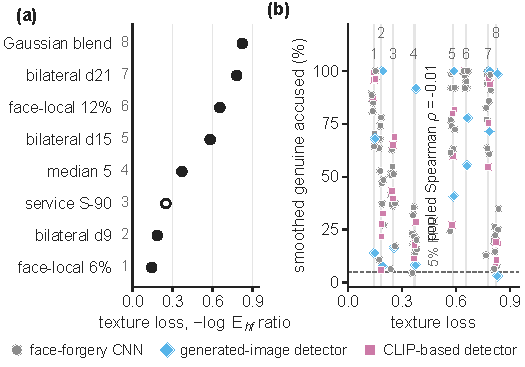
\includegraphics[width=3.5in]{fig_bandenergy_v8b}
\caption{The cue is the smoothing signature rather than blur. (a) Texture loss of eight smoothing forms, measured as the
high-frequency energy removed inside the face hull of 400 genuine Celeb-DF-v2 frames (commercial Smoothing-90 on 200 FFHQ
pairs, hollow). (b) False-alarm rate of each published detector at each form against that loss. A Gaussian blend removes the
most energy and is accused least; a face-local bilateral filter removes less and is accused by nearly every detector.}
% figs/fig_bandenergy_v8b.pdf (make_fig_bandenergy_v8b.py) from results/research/retouch_unified_20260929/bandenergy_20261018/
% bandenergy.json (loss_per_form.ehf0.25_view) and fa_parsed.json (published[*].fa) (BANDENERGY.md)
\label{fig:bandenergy}
\end{figure}

\section{Dose response of the CLIP detectors}
\label{sec:dose}
\begin{table}[H]
\centering
\caption{Released Effort, Forensics Adapter, GenD and DFD-HR on the 1,348 genuine frames of Sec.~\ref{sec:smooth38}. Cells: median
shift of the forgery logit (edited minus untreated) with a 95\% video-cluster interval (1,000 draws) / the shift in units of the
detector's gap between mean forged and mean genuine logit (in parentheses after the name). Vignette: radial darkening at strength
0.1 to 0.8; face-local smoothing at blend fraction 0.03 to 0.12; whole-crop bilateral at three strengths (light and strong shown).
Dose response (vignette / face-local / bilateral): the declared rule, a shift toward forged that grows with strength.}
\label{tab:dose}
\scriptsize
\begin{adjustbox}{max width=\linewidth}\begin{tabular}{@{}l cccccc c@{}}
\toprule
Detector (gap) & vignette 0.1 & vignette 0.8 & face-local 0.03 & face-local 0.12 & bil.\ light & bil.\ strong & dose response \\
\midrule
Effort (2.30) & -0.077 [-0.091, -0.064] / -0.03 & -0.205 [-0.254, -0.160] / -0.09 & +2.396 [+2.202, +2.561] / 1.04 & +4.327 [+4.175, +4.433] / 1.88 & +0.686 [+0.604, +0.737] / 0.30 & +2.280 [+2.125, +2.413] / 0.99 & no / yes / yes \\
Forensics Adapter (3.82) & -0.075 [-0.089, -0.057] / -0.02 & -0.359 [-0.428, -0.302] / -0.09 & +4.585 [+4.331, +4.874] / 1.20 & +9.786 [+9.519, +10.002] / 2.56 & +1.798 [+1.645, +1.977] / 0.47 & +4.734 [+4.462, +5.047] / 1.24 & no / yes / yes \\
GenD (2.89) & -0.074 [-0.086, -0.061] / -0.03 & -0.360 [-0.442, -0.281] / -0.12 & +3.382 [+3.205, +3.596] / 1.17 & +5.528 [+5.286, +5.700] / 1.91 & +1.816 [+1.627, +1.991] / 0.63 & +4.489 [+4.312, +4.660] / 1.55 & no / yes / yes \\
DFD-HR (2.05) & -0.001 [-0.010, +0.006] / -0.00 & +0.069 [+0.043, +0.095] / 0.03 & +3.961 [+3.805, +4.075] / 1.93 & +6.060 [+5.954, +6.182] / 2.96 & +0.900 [+0.845, +0.965] / 0.44 & +3.448 [+3.349, +3.571] / 1.68 & yes / yes / yes \\
\bottomrule
\end{tabular}
\end{adjustbox}
\end{table}
Under face-local smoothing the logit rises in at least 97.9\% of frames at every level for all four detectors; at the weakest level
61--89\% of genuine frames are already above the 5\%-FPR threshold, at the strongest 99.9--100\%. Under the vignette 18--60\% of
frames rise; Effort, Forensics Adapter and GenD move toward genuine, and DFD-HR passes the rule with a top-level median of $+0.07$
(3\% of its gap). The mean $|\cos|$ between the feature shift and the head direction is 0.04--0.39, except for Forensics Adapter's
192-dimensional head input (0.42--0.69).

\section{Identity-cluster bootstrap}
\label{sec:identity}
Units: Celeb-DF-B 464 videos in 58 identities; Celeb-DF-v2 filtered 516 videos in 124 units (59 celebrities and 65 YouTube-real
singletons); DFD 332 videos in 28 actors; DF40 FF++ domain 140 identities (the Celeb-DF domain has no identity labels and keeps
video units). The statistics, draws (1,000, rng 0) and thresholds are those of the paper; only the resampling unit changes. The
set tested is: on Celeb-DF-B the beautification-specific miss rise and FA$_b$ (against 0 and 5\%) of every detector and the paired
AUC$_b$ differences of our full-data models and of GenD and DFD-HR; on the four filter sources the miss and false-alarm rise of every
detector and the paired AUC$_f$ differences of our models; on DF40 the paired video-AUC differences of our full-data models. Of these
563 intervals, 24 change category (containing the null or excluding it; Table~\ref{tab:identity}). Identity intervals are 0.86
(Celeb-DF-B, narrower because a person's genuine and forged videos move together), 1.06--1.08 (Celeb-DF-v2), 1.00 (DFD) and 1.30
(DF40, up to 2.8) times as wide as the video intervals (median ratios). An earlier run without the second seeds, which also counted
the raw miss rise on Celeb-DF-B and a merged-identity variant, gave 20 of 456. No paired AUC$_b$ difference of our models against
the four CLIP detectors changes category: every identity interval of the full-data models has its lower bound at or above 0.008,
and those of P0 at or above 0.006 (Table~\ref{tab:cdfbpaired}, which uses the same identity draws).
\begin{table}[H]
\centering
\caption{The 24 of 563 intervals that change category when identities replace videos as the resampling unit.
d\_miss, d\_fa: rise under the filters; AUC\_f: frame AUC under the filters; DF40: video AUC, mean over face-swap (FS) or reenactment
(FR) methods, FF++ domain.}
\label{tab:identity}
\scriptsize
\begin{adjustbox}{max width=\linewidth}\begin{tabular}{@{}l l c c c l@{}}
\toprule
Source & quantity & estimate & video CI & identity CI & change \\
\midrule
Celeb-DF-B & caddm: d\_miss\_beauty\_only & -2.87 & [-5.770, -0.023] & [-5.924, +0.005] & below $\rightarrow$ contains \\
Celeb-DF-B & AUC\_b gend - fadapter & -0.0208 & [-0.045, +0.001] & [-0.041, -0.001] & contains $\rightarrow$ below \\
Celeb-DF-v2 + filters (crop) & srm: d\_miss & +1.51 & [+0.064, +3.269] & [-0.523, +3.848] & above $\rightarrow$ contains \\
Celeb-DF-v2 + filters (crop) & FF++-only three-way: d\_miss & +3.24 & [+0.403, +6.177] & [-0.193, +6.264] & above $\rightarrow$ contains \\
Celeb-DF-v2 + filters (crop) & AUC\_f \oursF{} - gend & +0.0316 & [+0.003, +0.060] & [-0.001, +0.063] & above $\rightarrow$ contains \\
Celeb-DF-v2 + filters (full frame) & effnb4: d\_miss & +2.47 & [+0.118, +4.921] & [-0.120, +5.433] & above $\rightarrow$ contains \\
Celeb-DF-v2 + filters (full frame) & AUC\_f \oursB{} - gend & +0.0273 & [+0.003, +0.051] & [-0.002, +0.054] & above $\rightarrow$ contains \\
Celeb-DF-v2 + filters (full frame) & AUC\_f sym.\ view - gend & +0.0249 & [+0.003, +0.046] & [-0.001, +0.049] & above $\rightarrow$ contains \\
Celeb-DF-v2 + filters (full frame) & AUC\_f FF++-only three-way - dfdhr & +0.0274 & [+0.004, +0.052] & [-0.002, +0.057] & above $\rightarrow$ contains \\
DFD + filters (crop) & AUC\_f \oursF{} - fadapter & +0.0197 & [+0.000, +0.042] & [-0.004, +0.041] & above $\rightarrow$ contains \\
DFD + filters (crop) & AUC\_f FF++-only three-way - fadapter & +0.0177 & [+0.000, +0.037] & [-0.002, +0.036] & above $\rightarrow$ contains \\
DFD + filters (full frame) & xception: d\_miss & +1.96 & [-0.688, +5.277] & [+0.190, +4.295] & contains $\rightarrow$ above \\
DFD + filters (full frame) & AUC\_f sym.\ view s2 - gend & +0.0145 & [-0.001, +0.030] & [+0.000, +0.028] & contains $\rightarrow$ above \\
DF40 & \oursF{} - gend: ff/FS & -0.0149 & [-0.023, -0.007] & [-0.030, +0.001] & below $\rightarrow$ contains \\
DF40 & \oursF{} s2 - effort: ff/FS & +0.0154 & [+0.006, +0.025] & [-0.006, +0.036] & above $\rightarrow$ contains \\
DF40 & \oursF{} s2 - effort: ff/FR & -0.0280 & [-0.045, -0.010] & [-0.070, +0.011] & below $\rightarrow$ contains \\
DF40 & \oursF{} s2 - fadapter: ff/FS & +0.0117 & [+0.003, +0.021] & [-0.005, +0.029] & above $\rightarrow$ contains \\
DF40 & \oursB{} - effort: ff/FR & +0.0343 & [+0.017, +0.051] & [-0.005, +0.076] & above $\rightarrow$ contains \\
DF40 & sym.\ view s2 - effort: ff/FS & +0.0137 & [+0.004, +0.024] & [-0.007, +0.035] & above $\rightarrow$ contains \\
DF40 & sym.\ view s2 - fadapter: ff/FS & +0.0099 & [+0.002, +0.019] & [-0.005, +0.027] & above $\rightarrow$ contains \\
DF40 & sym.\ view s2 - gend: ff/FS & -0.0086 & [-0.016, -0.001] & [-0.023, +0.005] & below $\rightarrow$ contains \\
DF40 & \oursB{} s2 - effort: ff/FS & +0.0172 & [+0.009, +0.027] & [-0.001, +0.035] & above $\rightarrow$ contains \\
DF40 & \oursB{} s2 - fadapter: ff/FS & +0.0135 & [+0.005, +0.022] & [-0.001, +0.029] & above $\rightarrow$ contains \\
DF40 & \oursB{} s2 - fadapter: ff/FR & +0.0281 & [+0.014, +0.041] & [-0.006, +0.064] & above $\rightarrow$ contains \\
\bottomrule
\end{tabular}
\end{adjustbox}
\end{table}

\section{The decomposition of a commercial render}
\label{sec:decomp}
Algorithm~\ref{alg:decomp}: dense optical flow on locally normalised luminance gives the warp $f$ between an original $O$ and its
render $R$, the photometric residual is taken in the geometry of $O$, and four single-operation components are formed, each with
its measured strength and exact footprint. Applying the four in sequence reproduces $R$ at 108\,dB PSNR.
\begin{algorithm}[H]
\caption{Single-operation components of a commercial render}
\label{alg:decomp}
\begin{algorithmic}[1]
\Require original $O$, render $R$, eye mask $E$, $\sigma$, noise floors $\tau_k$
\State $f\gets\mathrm{DIS}\big(\mathrm{LCN}(O),\mathrm{LCN}(R)\big)$
\State $P\gets R\circ(\mathrm{id}-f^{-1}) - O$
\State $C_\text{eye}\gets\mathcal{W}(O;E\odot f)$;\quad $C_\text{contour}\gets\mathcal{W}(O;(1-E)\odot f)$
\State $C_\text{tone}\gets O+G_\sigma*P$;\quad $C_\text{texture}\gets O+P-G_\sigma*P$
\For{$k\in\{\text{eye},\text{contour},\text{tone},\text{texture}\}$}
  \State $q_k\gets\mathrm{Measure}_k(C_k,O)$;\ \textbf{if} $q_k\ge\tau_k$ \textbf{keep} $(C_k,\ e_k,\ M(C_k))$
\EndFor
\end{algorithmic}
\end{algorithm}
The loss is $\mathcal{L}=\mathrm{BCE}(z_f,y_f)+\mathrm{BCE}(z_b,y_b)+\mathbf{1}[y_b]\,\mathrm{BCE}(\hat s,s)+\mathbf{1}[M\
\text{exact}]\,\big(\mathrm{BCE}(\hat m,M)+\mathrm{Dice}(\hat m,M)\big)$, with $\hat s$ the operation-presence logits.

\section{Exposure arms on every source}
\label{sec:exposure}
\begin{table}[H]
\centering
\caption{Which class receives beautified training views. FF++ only, forged head only, everything else identical; three seeds.
Celeb-DF-B under the one rule of the paper.}
\label{tab:exposure}
\footnotesize
\begin{adjustbox}{max width=\linewidth}\begin{tabular}{@{}llccc@{}}
\toprule
Arm & Beautified training views & AUC$_b$ (3 seeds) & $\Delta$MISS$_\text{beauty}$ (3 seeds) & FA$_b$ \\
\midrule
P0 & no beautified views & 0.860 / 0.883 / 0.883 & +17.0 / +14.2 / +10.8 & 5.1 / 5.6 / 6.8 \\
P1 & beautified genuine faces only & 0.844 / 0.851 / 0.864 & +21.5 / +21.8 / +20.4 & 4.5 / 3.9 / 3.7 \\
P2 & beautified genuine and forged faces & 0.879 / 0.893 / 0.877 & +9.8 / +10.3 / +12.8 & 5.6 / 5.3 / 5.4 \\
\midrule
\multicolumn{5}{@{}l}{Paired differences, 95\% video-cluster intervals (seeds 1 / 2 / 3)} \\
P1 $-$ P0 & $\Delta$MISS$_\text{beauty}$ & \multicolumn{3}{l}{+4.5 [1.5, 7.6] / +7.5 [4.4, 10.8] / +9.5 [6.7, 12.3]} \\
P2 $-$ P0 & $\Delta$MISS$_\text{beauty}$ & \multicolumn{3}{l}{-7.2 [-9.4, -5.0] / -4.0 [-6.1, -2.0] / +2.0 [0.1, 4.0]} \\
P2 $-$ P1 & $\Delta$MISS$_\text{beauty}$ & \multicolumn{3}{l}{-11.7 [-14.5, -8.8] / -11.5 [-14.5, -8.9] / -7.5 [-10.0, -5.0]} \\
\bottomrule
\end{tabular}
\end{adjustbox}
\end{table}
\begin{table}[H]
\centering
\caption{P0 none, P1 genuine only, P2 both; FF++ only, forged head only; values per seed. Effort scheme: the SVD-residual tuning
of the released Effort code in place of LoRA; P1 was not trained under it. Frame AUC; $\Delta$MISS at the 5\%-FPR threshold of
untreated genuine frames.}
\label{tab:exposure_ext}
\footnotesize
\begin{adjustbox}{max width=\linewidth}\begin{tabular}{@{}ll ccc cc cc@{}}
\toprule
 & & \multicolumn{3}{c}{Celeb-DF-B} & \multicolumn{2}{c}{Celeb-DF-v2 filters} & \multicolumn{2}{c}{DFD filters} \\
\cmidrule(lr){3-5}\cmidrule(lr){6-7}\cmidrule(lr){8-9}
Tuning & Arm & AUC & AUC$_b$ & $\Delta$MISS$_\text{beauty}$ & AUC$_f$ & $\Delta$MISS & AUC$_f$ & $\Delta$MISS \\
\midrule
LoRA & P0 & 0.927 / 0.937 / 0.944 & 0.860 / 0.883 / 0.883 & +17.0 / +14.2 / +10.8 & 0.852 / 0.858 / 0.855 & +7.1 / +4.4 / +8.3 & 0.924 / 0.928 / 0.932 & +9.3 / +7.2 / +8.7 \\
LoRA & P1 & 0.928 / 0.931 / 0.939 & 0.844 / 0.851 / 0.864 & +21.5 / +21.8 / +20.4 & 0.798 / 0.820 / 0.838 & +16.6 / +17.7 / +16.3 & 0.905 / 0.911 / 0.913 & +11.2 / +9.3 / +9.2 \\
LoRA & P2 & 0.929 / 0.933 / 0.935 & 0.879 / 0.893 / 0.877 & +9.8 / +10.3 / +12.8 & 0.848 / 0.850 / 0.856 & +0.3 / +3.0 / -0.9 & 0.929 / 0.929 / 0.927 & +2.5 / +1.8 / -0.5 \\
\midrule
Effort scheme & P0 & 0.943 / 0.948 & 0.882 / 0.886 & +10.1 / +10.7 & 0.876 / 0.886 & +2.3 / -1.3 & 0.942 / 0.947 & +8.7 / +7.4 \\
Effort scheme & P2 & 0.938 / 0.943 & 0.889 / 0.890 & +5.5 / +5.5 & 0.872 / 0.879 & -7.6 / -8.4 & 0.948 / 0.953 & +3.0 / +2.4 \\
\bottomrule
\end{tabular}
\end{adjustbox}
\end{table}
Bootstrap $p$-values for the nine exposure contrasts on Celeb-DF-B (P1$-$P0, P2$-$P0 and P2$-$P1 on
$\Delta$MISS$_\text{beauty}$, three seeds, 1,000 identical video draws, $p=2\min(\Pr[d\le0],\Pr[d\ge0])$ floored at $10^{-3}$),
Holm-adjusted over the nine: P1$-$P0 is $+4.5$, $+7.5$ and $+9.5$ points (adjusted $p=0.009$ each); P2$-$P1 is $-11.7$, $-11.5$ and
$-7.5$ (0.009 each); P2$-$P0 is $-7.2$ and $-4.0$ (0.009) and $+2.0$ on the third seed (0.044). The family-wise picture is the one the
paper states: P1 is worse than P0 and P2 in every seed, and P2 against P0 changes sign across seeds.
Paired video-cluster intervals for P2 minus P0 on the two filter sources: the miss rise falls by 5.0 to 9.9 points in nine of ten
seed-by-source cells (intervals below zero; the tenth is $-1.4$ $[-3.3, 0.6]$), the false-alarm rise grows by 2.0 to 4.6 points in
the same nine, and the frame AUC under the filters changes by $-0.008$ to $+0.006$ (intervals contain zero except for the Effort
scheme on DFD, $+0.006$). For P1 minus P0 on Celeb-DF-v2 the miss rise grows by 13.3 and 8.0 points and the AUC under the filters
falls by 0.038 and 0.017.

\section{The forged-only arm}
\label{sec:p3}
\begin{table}[H]
\centering
\caption{The four exposure arms, seed 20260929: Smoothing-90 accused at the 5\%-FPR threshold of the originals with a 95\%
interval over originals, share of renders above their own original, false alarms on whole-crop- and skin-only-smoothed genuine
Celeb-DF-v2 frames (\%), and DF40 reenactment video AUC (FF++ / Celeb-DF domain). P1 was not scored on the skin-only forms
(P1-smooth: 0.4 and 0.0\%).}
\label{tab:p3}
\scriptsize
\begin{adjustbox}{max width=\linewidth}\begin{tabular}{@{}l c c c c c@{}}
\toprule
Arm & Smoothing-90 accused (\%) [CI] & above own (\%) & FA bil.\ light/mid/strong/med./blend & face-local 0.06/0.12 & DF40 FR ff / cdf \\
\midrule
P0 & 54.2 [50.5, 58.3] & 98.5 & 0.8 / 16.8 / 39.6 / 1.5 / 5.5 & 95.8 / 100.0 & 0.906 / 0.692 \\
P1 & 3.7 [2.9, 4.4] & 43.5 & 0.0 / 0.0 / 0.0 / 0.7 / 4.7 & -- & 0.807 / 0.569 \\
P2 & 11.7 [9.7, 14.3] & 84.1 & 3.0 / 31.8 / 49.1 / 2.5 / 3.3 & 38.6 / 74.5 & 0.809 / 0.644 \\
P3 & 63.8 [59.0, 67.8] & 99.2 & 59.6 / 99.5 / 100.0 / 18.8 / 6.2 & 98.1 / 100.0 & 0.870 / 0.753 \\
\bottomrule
\end{tabular}
\end{adjustbox}
\end{table}
Declared reading: (i) the sign rule is complete if P3 minus P0 on Smoothing-90 is not wholly below $-5$ and P3's false alarms on
mid and strong whole-crop-smoothed genuine frames are not lower than P0's; (ii) forged-only views also remove the accusation if
P3 accuses at most 15\%. P3 minus P0 is $+9.6$ [$+6.0$, $+13.4$] (P3 minus P2 $+52.1$ [$+47.5$, $+55.8$]) and the false alarms are
99.5 and 100\% against 16.8 and 39.6\%: (i) holds, (ii) does not. P3 mirrors P1: forgeries under the filters are missed less often
than untreated ones ($-25.1$ points on Celeb-DF-v2, $-6.6$ on DFD, against $+4.4$ and $+8.5$ for P0), the miss rate on beautified
Celeb-DF-B forgeries rises by 1.0 point (P0 $+23.3$), and beautified Celeb-DF-B genuine frames are accused at 24.6\% (P0 5.1\%).
Untreated detection is not lower: Celeb-DF-v2 video AUC 0.943 (P0 0.938), DFD 0.982 (0.981), DF40 face swap 0.970 and 0.937. On
the service, its native decision sends 93.9\% of the Smoothing-90 renders to forged. One seed.

\section{The colour-filter probe, per filter}
\label{sec:probe}
The probed model is the FF++-only three-way CLIP model (``FF++-only three-way'' in Tables~\ref{tab:twosidedfull} and~\ref{tab:cdfbextra}), trained with random
colour grading and 14 colour filters as beautified views; the training-time subspace below exists because those views were in
its training. No published detector was probed with this subspace analysis. The dose response of the released CLIP detectors
(Sec.~\ref{sec:dose}) shows that a vignette in isolation does not move three of them toward forged, so the radial-overlay effect
below is a property of this model, not a general account of the filter result.
\begin{table}[H]
\centering
\caption{FF++ validation frames under the eleven held-out filters: cosine of the mean feature shift with the forged weight vector
$w$, mean change of the forged logit on genuine and forged frames, and share of the shift energy inside the 16-dimensional
subspace spanned by training-time beautifications.}
\label{tab:mechanism}
\footnotesize
\begin{tabular}{@{}lrrrrr@{}}
\toprule
Held-out filter & $n$ & $\cos(w,\bar\Delta)$ & $\Delta$logit genuine & $\Delta$logit forged & energy in $V_{16}$ \\
\midrule
earlybird & 88 & 0.20 & +7.84 & +1.10 & 0.86 \\
mayfair & 94 & 0.33 & +5.64 & +1.80 & 0.83 \\
kelvin & 92 & 0.04 & +2.40 & -0.71 & 0.90 \\
clarendon & 99 & 0.07 & +1.90 & +0.40 & 0.86 \\
lofi & 95 & 0.06 & +1.86 & +0.17 & 0.87 \\
moon & 89 & 0.06 & +1.75 & -0.10 & 0.75 \\
perpetua & 107 & 0.09 & +0.99 & +0.21 & 0.77 \\
inkwell & 95 & 0.09 & +0.86 & -0.25 & 0.63 \\
reyes & 104 & 0.02 & +0.76 & -0.27 & 0.89 \\
slumber & 101 & 0.00 & +0.43 & -0.28 & 0.87 \\
brooklyn & 95 & 0.00 & +0.14 & -0.04 & 0.88 \\
\bottomrule
\end{tabular}

\end{table}
\begin{figure}[H]
\centering
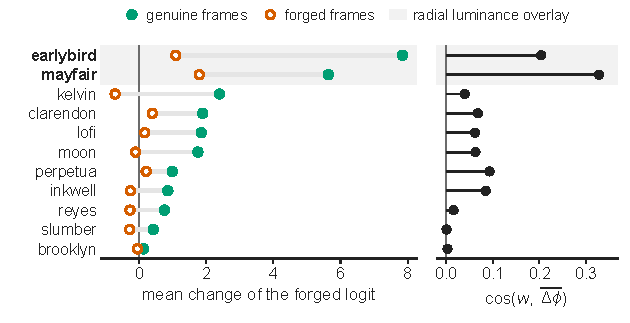
\includegraphics[width=4.2in]{fig_mechanism}
\caption{Mean change of the forged logit under each held-out filter on genuine (filled) and forged (open) frames (left), and
cosine of the mean feature shift with $w$ (right). Shaded rows: the two filters with a radial luminance overlay.}
\label{fig:mechanism}
\end{figure}
\begin{table}[H]
\centering
\caption{Linear erasure. The feature shifts caused by training-time beautifications are decomposed by SVD on training frames,
the first $k$ directions are projected out, and a logistic forged head is refitted on training features. FA and MISS at the
5\%-FPR threshold of clean genuine frames, pooled over the eleven held-out filters. The control is the refit without erasure
($k=0$), not the trained head.}
\label{tab:erasure}
\footnotesize
\begin{tabular}{@{}lcccc@{}}
\toprule
Forged head & AUC clean & AUC filtered & FA filtered & MISS filtered \\
\midrule
trained head & 0.987 & 0.953 & 21.5 & 5.9 \\
refit, 0 directions erased & 0.985 & 0.916 & 15.8 & 16.6 \\
refit, 2 directions erased & 0.933 & 0.907 & 18.5 & 15.1 \\
refit, 8 directions erased & 0.932 & 0.844 & 18.3 & 27.6 \\
refit, 32 directions erased & 0.919 & 0.804 & 19.2 & 32.1 \\
\bottomrule
\end{tabular}

\end{table}
The two leading directions hold 79\% of the shift energy of training-time beautifications. Against the refit without erasure,
removing them costs 0.052 clean AUC and raises the pooled false alarms under the filters from 15.8 to 18.5\% (18.3 and 19.2\% for
8 and 32 directions); per filter the false-alarm rate after erasure ranges from 17.5 to 27.5\%. The directions along which
beautification moves the feature carry forgery evidence for this model.

\section{Skin smoothing: the chain of pre-registered arms}
\label{sec:chain}
All arms are FF++-only models with the forged head only; they share the architecture, data, steps and checkpoint rule of the
exposure arms and differ only in which class receives beautified views and what those views contain. No image of any retouching
service is used. The scripted smoothing is a bilateral filter blended inside a feathered face hull, the same kind of edit as the
service's (face-local and edge-preserving: high-frequency energy on flat skin 0.68 at the top of the training range against 0.60
for the service's level 90, background 1.00 against 0.96). Its strength range was set to cover the levels measured on the two
sister services in RetouchingFFHQ while the test service's measurements were on disk.

\begin{table}[H]
\centering
\caption{Commercial skin smoothing, every detector and arm: 2,210 FFHQ originals and their renders. Smoothing-90: share of renders
scored above their own original (50 means no shift), medians of $P(\text{fake})$, and share above the threshold that accuses 5\% of
the originals. All renders: the four operations at three levels (26,519 images). NPR scores originals and renders at 1.0.}
\label{tab:v4retouch}\label{tab:retouch}
\scriptsize
\begin{adjustbox}{max width=\linewidth}\begin{tabular}{@{}l ccc cc@{}}
\toprule
 & \multicolumn{3}{c}{Smoothing-90 renders} & \multicolumn{2}{c}{all renders} \\
\cmidrule(lr){2-4}\cmidrule(lr){5-6}
Detector & above own original (\%) & median $P(\text{fake})$ orig.\ $\rightarrow$ render & above 5\%-FPR thr.\ (\%) & above 5\%-FPR thr.\ (\%) & AUROC render vs orig. \\
\midrule
Xception~\cite{xception} & 95.2 & 0.291 $\rightarrow$ 0.944 & 51.6 & 12.2 & 0.563 \\
EfficientNet-B4~\cite{efficientnet} & 93.7 & 0.316 $\rightarrow$ 0.964 & 36.3 & 9.4 & 0.545 \\
F3Net~\cite{f3net} & 97.8 & 0.131 $\rightarrow$ 0.974 & 50.6 & 11.8 & 0.568 \\
SPSL~\cite{spsl} & 97.3 & 0.463 $\rightarrow$ 0.963 & 51.2 & 12.1 & 0.567 \\
UCF~\cite{ucf} & 95.4 & 0.031 $\rightarrow$ 0.984 & 41.4 & 11.2 & 0.575 \\
RECCE~\cite{recce} & 96.5 & 0.120 $\rightarrow$ 0.944 & 36.8 & 9.5 & 0.558 \\
CORE~\cite{core} & 96.6 & 0.249 $\rightarrow$ 0.947 & 54.8 & 12.4 & 0.569 \\
SRM~\cite{srm} & 99.3 & 0.461 $\rightarrow$ 0.668 & 62.8 & 13.9 & 0.570 \\
SBI~\cite{sbi} & 96.2 & 0.208 $\rightarrow$ 0.991 & 37.3 & 11.3 & 0.582 \\
UnivFD$^\ddagger$~\cite{univfd} & 90.4 & 0.005 $\rightarrow$ 0.019 & 16.6 & 7.3 & 0.526 \\
NPR$^\ddagger$~\cite{npr} & n/a (saturated) & n/a & n/a & n/a & n/a \\
Effort~\cite{effort} & 95.6 & 0.319 $\rightarrow$ 0.595 & 43.2 & 14.8 & 0.599 \\
Forensics Adapter~\cite{forensicsadapter} & 93.3 & 0.058 $\rightarrow$ 0.354 & 39.7 & 10.2 & 0.541 \\
GenD~\cite{gend2026} & 98.5 & 0.228 $\rightarrow$ 0.921 & 68.7 & 16.8 & 0.596 \\
DFD-HR~\cite{dfdhr2026} & 99.0 & 0.210 $\rightarrow$ 0.711 & 64.9 & 15.7 & 0.554 \\
CADDM~\cite{caddm} & 60.9 & 0.538 $\rightarrow$ 0.745 & 6.3 & 5.6 & 0.523 \\
LAA-Net~\cite{laanet} & 89.2 & 0.234 $\rightarrow$ 0.969 & 17.2 & 7.6 & 0.578 \\
\midrule
\oursB{} & 70.5 & 0.000 $\rightarrow$ 0.001 & 9.1 & 5.2 & 0.490 \\
\oursF{} & 32.5 & 0.002 $\rightarrow$ 0.001 & 8.6 & 4.7 & 0.371 \\
\oursF{}, sym.\ view & 30.0 & 0.003 $\rightarrow$ 0.001 & 8.1 & 4.8 & 0.375 \\
\midrule
\multicolumn{6}{@{}l}{FF++-only exposure arms (seed 1)} \\
\quad P0 & 98.5 & 0.049 $\rightarrow$ 0.968 & 54.2 & 13.5 & 0.576 \\
\quad P2 & 84.1 & 0.009 $\rightarrow$ 0.116 & 11.7 & 5.9 & 0.528 \\
\quad P2 no smoothing & 98.6 & 0.017 $\rightarrow$ 0.988 & 55.3 & 12.7 & 0.553 \\
\quad P2 smoothing only & 27.3 & 0.053 $\rightarrow$ 0.020 & 2.3 & 3.7 & 0.449 \\
\quad P1 & 43.5 & 0.004 $\rightarrow$ 0.004 & 3.7 & 5.3 & 0.500 \\
\quad P1 smoothing only & 2.6 & 0.074 $\rightarrow$ 0.000 & 0.7 & 4.9 & 0.437 \\
\quad P2 symmetric smoothing & 53.7 & 0.017 $\rightarrow$ 0.022 & 5.9 & 4.9 & 0.488 \\
\midrule
\multicolumn{6}{@{}l}{FF++ only, Effort's tuning scheme (seed 1)} \\
\quad Effort scheme, no beautified views & 99.1 & 0.028 $\rightarrow$ 0.963 & 56.9 & 13.3 & 0.587 \\
\quad Effort scheme, symmetric smoothing & 88.4 & 0.029 $\rightarrow$ 0.095 & 14.5 & 7.2 & 0.541 \\
\quad released Effort fine-tuned, no beautified views & 98.5 & 0.091 $\rightarrow$ 0.306 & 55.3 & 14.4 & 0.564 \\
\quad released Effort fine-tuned, symmetric smoothing & 96.6 & 0.080 $\rightarrow$ 0.174 & 39.9 & 11.5 & 0.553 \\
\bottomrule
\end{tabular}
\end{adjustbox}
\end{table}
\begin{table}[H]
\centering
\caption{Paired shift of the forgery logit, Smoothing-90 render minus its own original (2,210 pairs): counts of pairs moving up and
down, median shift with a 95\% bootstrap interval over originals (1,000 draws), and the two-sided sign test with ties dropped.
Probabilities are clipped to $[10^{-7}, 1-10^{-7}]$ before the logit. NPR is saturated and omitted.}
\label{tab:shiftall}
\footnotesize
\begin{tabular}{@{}l ccc@{}}
\toprule
Model & up / down / tie & median $\Delta$logit [95\% CI] & sign test $p$ \\
\midrule
Xception~\cite{xception} & 2105 / 105 / 0 & +3.32 [+3.17, +3.45] & $<10^{-10}$ \\
EfficientNet-B4~\cite{efficientnet} & 2070 / 140 / 0 & +3.48 [+3.33, +3.57] & $<10^{-10}$ \\
F3Net~\cite{f3net} & 2161 / 49 / 0 & +4.92 [+4.74, +5.08] & $<10^{-10}$ \\
SPSL~\cite{spsl} & 2151 / 59 / 0 & +3.05 [+2.95, +3.12] & $<10^{-10}$ \\
UCF~\cite{ucf} & 2108 / 102 / 0 & +5.47 [+5.20, +5.73] & $<10^{-10}$ \\
RECCE~\cite{recce} & 2133 / 77 / 0 & +3.82 [+3.70, +3.96] & $<10^{-10}$ \\
CORE~\cite{core} & 2135 / 75 / 0 & +3.90 [+3.74, +4.03] & $<10^{-10}$ \\
SRM~\cite{srm} & 2194 / 16 / 0 & +0.68 [+0.65, +0.71] & $<10^{-10}$ \\
SBI~\cite{sbi} & 2127 / 83 / 0 & +4.88 [+4.72, +5.04] & $<10^{-10}$ \\
UnivFD$^\ddagger$~\cite{univfd} & 1998 / 212 / 0 & +1.22 [+1.17, +1.28] & $<10^{-10}$ \\
Effort~\cite{effort} & 2113 / 97 / 0 & +0.96 [+0.90, +1.02] & $<10^{-10}$ \\
Forensics Adapter~\cite{forensicsadapter} & 2063 / 147 / 0 & +1.72 [+1.59, +1.87] & $<10^{-10}$ \\
GenD~\cite{gend2026} & 2176 / 34 / 0 & +3.27 [+3.19, +3.35] & $<10^{-10}$ \\
DFD-HR~\cite{dfdhr2026} & 2189 / 21 / 0 & +2.06 [+1.93, +2.15] & $<10^{-10}$ \\
CADDM~\cite{caddm} & 1345 / 865 / 0 & +0.67 [+0.53, +0.81] & $<10^{-10}$ \\
LAA-Net~\cite{laanet} & 1971 / 239 / 0 & +3.60 [+3.36, +3.79] & $<10^{-10}$ \\
\midrule
\oursB{} & 1557 / 642 / 11 & +0.41 [+0.38, +0.44] & $<10^{-10}$ \\
\quad second seed & 1508 / 694 / 8 & +0.19 [+0.16, +0.19] & $<10^{-10}$ \\
\oursF{} & 718 / 1490 / 2 & -1.20 [-1.28, -1.12] & $<10^{-10}$ \\
\quad second seed & 913 / 1296 / 1 & -0.53 [-0.60, -0.41] & $<10^{-10}$ \\
\oursF{}, sym.\ view & 662 / 1545 / 3 & -1.09 [-1.19, -1.00] & $<10^{-10}$ \\
P0 & 2176 / 34 / 0 & +5.17 [+5.05, +5.38] & $<10^{-10}$ \\
P2 & 1859 / 347 / 4 & +1.81 [+1.68, +1.97] & $<10^{-10}$ \\
P1 & 962 / 1245 / 3 & -0.22 [-0.28, -0.16] & $1.8\times10^{-9}$ \\
P1-smooth & 57 / 2153 / 0 & -5.00 [-5.16, -4.88] & $<10^{-10}$ \\
P2-smooth & 604 / 1602 / 4 & -0.91 [-0.97, -0.84] & $<10^{-10}$ \\
P2-sym & 1187 / 1017 / 6 & +0.09 [+0.03, +0.12] & $3.2\times10^{-4}$ \\
\quad P2-sym, seed 2 & 1144 / 1059 / 7 & +0.03 [-0.00, +0.09] & 0.07 \\
\bottomrule
\end{tabular}

\end{table}
The published detectors and the no-exposure arm move the logit of a smoothed genuine face up by 0.7 to 5.5. \oursF{}, its variant
and the genuine-only or form-asymmetric arms move it down, which is the evasion direction; \oursB{} moves it up by 0.41 and 0.19
(two seeds). Only P2-sym is close to no shift, with a small upward median on its first seed ($p=3.2\times10^{-4}$) and none detectable on
its second ($p=0.07$). A 25--75\% band on the share of pairs, the bar used for P2-sym and the variant, is wide: it admits \oursF{}'s
32.5\%, which the sign test shows is a shift.

\begin{sidewaystable}
\centering
\caption{The exposure table of the paper (Table~\ref{M-tab:exposure}) with every column; values per seed (1 / 2 / 3 where trained).
Arm names in the paper: P2 no smoothing = P2-nosmooth, P2 smoothing only = P2-smooth, P1 smoothing only = P1-smooth, P2 symmetric
smoothing = P2-sym. Untreated video AUC; Celeb-DF-B frame AUC; DF40 reenactment video AUC.}
\label{tab:tradeofffull}
\scriptsize
\begin{adjustbox}{max width=\linewidth}\begin{tabular}{@{}l cc cc cc cc cc@{}}
\toprule
 & \multicolumn{2}{c}{commercial Smoothing-90} & \multicolumn{2}{c}{smoothed Celeb-DF-v2 (strong bil.)} & \multicolumn{2}{c}{untreated video AUC} & \multicolumn{2}{c}{Celeb-DF-B (frame)} & \multicolumn{2}{c}{DF40 FR video AUC} \\
\cmidrule(lr){2-3}\cmidrule(lr){4-5}\cmidrule(lr){6-7}\cmidrule(lr){8-9}\cmidrule(lr){10-11}
Arm & accused (\%) & above own orig.\ (\%) & miss rise & frame AUC, both smoothed & Celeb-DF-v2 & DFD & AUC$_b$ & $\Delta$MISS$_\text{beauty}$ & FF++ dom. & Celeb-DF dom. \\
\midrule
P0 & 54.2 / 56.1 / 43.5 & 98.5 / 99.0 / 97.0 & -16.0 / -11.8 / +4.3 & 0.747 / 0.736 / 0.736 & 0.938 / 0.938 / 0.940 & 0.981 / 0.979 / 0.978 & 0.860 / 0.883 / 0.883 & +17.0 / +14.2 / +10.8 & 0.906 / 0.877 / 0.873 & 0.692 / 0.720 / 0.633 \\
P1 & 3.7 / 7.1 / 4.6 & 43.5 / 67.5 / 64.3 & +51.2 / -- / -- & 0.587 / -- / -- & 0.900 / 0.910 / 0.923 & 0.978 / 0.975 / 0.971 & 0.844 / 0.851 / 0.864 & +21.5 / +21.8 / +20.4 & 0.807 / -- / -- & 0.569 / -- / -- \\
P2 & 11.7 / 7.1 / 6.9 & 84.1 / 72.4 / 75.5 & -26.5 / -13.3 / -- & 0.740 / 0.746 / -- & 0.917 / 0.920 / 0.935 & 0.973 / 0.975 / 0.972 & 0.879 / 0.893 / 0.877 & +9.8 / +10.3 / +12.8 & 0.809 / 0.785 / -- & 0.644 / 0.643 / -- \\
P3 & 63.8 & 99.2 & -38.5 & 0.743 & 0.943 & 0.982 & 0.857 & -2.3 & 0.870 & 0.753 \\
P2-nosmooth & 55.3 / 67.1 & 98.6 / 99.4 & -28.9 / -33.1 & 0.732 / 0.695 & 0.913 / 0.924 & 0.980 / 0.973 & 0.879 / 0.873 & +12.9 / +12.9 & 0.858 / -- & 0.705 / -- \\
P2-smooth & 2.3 / 5.3 & 27.3 / 51.7 & -48.2 / -44.6 & 0.785 / 0.734 & 0.904 / 0.926 & 0.967 / 0.966 & 0.865 / 0.870 & +10.2 / +13.7 & 0.779 / 0.833 & 0.593 / 0.629 \\
P1-smooth & 0.7 / 1.0 / 0.9 & 2.6 / 6.5 / 5.4 & +56.4 / +60.0 / +62.9 & 0.643 / 0.579 / 0.596 & 0.922 / 0.929 / 0.939 & 0.974 / 0.977 / 0.964 & 0.887 / 0.896 / 0.893 & +8.6 / +8.5 / +7.3 & 0.871 / 0.869 / 0.900 & 0.673 / 0.689 / 0.679 \\
P2-sym & 5.9 / 6.1 & 53.7 / 51.8 & +14.6 / +17.5 & 0.767 / 0.796 & 0.919 / 0.934 & 0.972 / 0.968 & 0.866 / 0.888 & +14.2 / +10.4 & 0.871 / 0.796 & 0.670 / 0.646 \\
Effort scheme, P0 & 56.9 / 63.2 & 99.1 / 99.1 & -32.2 / -- & 0.719 / -- & 0.944 / 0.954 & 0.987 / 0.991 & 0.882 / 0.886 & +10.1 / +10.7 & -- / -- & -- / -- \\
Effort scheme, P2-sym & 14.5 & 88.4 & +24.9 & 0.757 & 0.935 & 0.986 & 0.890 & +10.6 & 0.822 & 0.614 \\
released Effort fine-tuned, no views & 55.3 & 98.5 & -39.9 & 0.754 & 0.926 & 0.976 & 0.805 & +5.8 & -- & -- \\
released Effort fine-tuned, P2-sym view & 39.9 & 96.6 & -19.0 & 0.740 & 0.921 & 0.974 & 0.791 & +7.5 & 0.805 & 0.705 \\
\oursB{} & 9.1 / 6.5 & 70.5 / 68.2 & -15.0 / +2.2 & 0.754 / 0.810 & 0.956 / 0.963 & 0.987 / 0.978 & 0.896 / 0.904 & +7.0 / +5.7 & 0.842 / 0.856 & 0.647 / 0.698 \\
\oursF{} & 8.6 / 12.5 & 32.5 / 41.3 & -44.3 / -46.7 & 0.688 / 0.711 & 0.947 / 0.946 & 0.978 / 0.981 & 0.866 / 0.883 & +6.7 / +8.3 & 0.718 / 0.780 & 0.502 / 0.559 \\
\oursF{}, sym.\ view & 8.1 / 17.8 & 30.0 / 46.2 & +34.1 / +11.6 & 0.796 / 0.784 & 0.954 / 0.953 & 0.983 / 0.987 & 0.868 / 0.888 & +10.0 / +3.1 & 0.738 / 0.718 & 0.539 / 0.504 \\
\bottomrule
\end{tabular}
\end{adjustbox}
\end{sidewaystable}

\begin{sidewaystable}
\centering
\caption{Smoothed forgeries and smoothed genuine frames. Celeb-DF-v2 test frames (every fourth of the 32 per video), untreated and
under a whole-crop bilateral filter at three strengths, a $5\times5$ median filter and a 50\% blend with a Gaussian blur; the last
two forms were shown to no arm. Threshold at 5\% FPR on untreated genuine frames. Miss rise: change of the miss rate on forgeries
after smoothing, with 95\% video-cluster intervals. Last column: frame AUC with both classes under the strong bilateral filter.}
\label{tab:v4evasion}
\scriptsize
\begin{adjustbox}{max width=\linewidth}\begin{tabular}{@{}l c ccccc ccccc c@{}}
\toprule
 & & \multicolumn{5}{c}{miss rise (points, 95\% CI)} & \multicolumn{5}{c}{false alarms, smoothed genuine (\%)} & \\
\cmidrule(lr){3-7}\cmidrule(lr){8-12}
Arm & miss untr.\ & bil.\ light & bil.\ mid & bil.\ strong & median 5 & Gauss.\ blend & bil.\ light & bil.\ mid & bil.\ strong & median 5 & Gauss.\ blend & AUC both smoothed (strong) \\
\midrule
P0 & 42.2 & +27.0 [+24.4, +29.7] & +5.1 [-0.3, +10.5] & -16.0 [-21.5, -10.2] & +19.2 [+17.1, +21.2] & +3.0 [+1.4, +5.1] & 0.8 & 16.8 & 39.6 & 1.5 & 5.5 & 0.747 \\
\quad seed 2 & 37.7 & +26.7 [+24.1, +29.9] & +6.1 [+2.2, +11.8] & -11.8 [-15.5, -5.4] & +18.0 [+16.0, +20.4] & +8.1 [+6.6, +9.9] & 1.6 & 18.2 & 42.9 & 1.9 & 4.4 & 0.736 \\
\quad seed 3 & 36.7 & +24.0 [+21.4, +26.9] & +14.3 [+8.8, +17.9] & +4.3 [-2.4, +11.0] & +12.6 [+10.6, +14.6] & +5.6 [+4.2, +6.9] & 2.3 & 11.3 & 25.2 & 3.0 & 4.9 & 0.736 \\
P2 & 46.8 & +16.5 [+14.2, +19.4] & -17.4 [-20.7, -13.1] & -26.5 [-29.7, -21.9] & +13.2 [+11.7, +15.8] & +7.0 [+6.0, +8.9] & 3.0 & 31.8 & 49.1 & 2.5 & 3.3 & 0.740 \\
P2 no smoothing & 46.7 & +19.8 [+16.8, +22.0] & -12.2 [-16.3, -6.5] & -28.9 [-32.8, -24.9] & +8.1 [+6.4, +9.8] & +2.2 [+0.7, +3.5] & 2.3 & 25.6 & 54.4 & 3.9 & 4.7 & 0.732 \\
P2 smoothing only & 49.5 & -34.3 [-37.6, -30.4] & -47.3 [-51.6, -40.2] & -48.2 [-53.1, -40.8] & +17.2 [+14.7, +20.2] & +10.9 [+9.2, +13.6] & 47.8 & 82.3 & 88.3 & 1.7 & 2.4 & 0.785 \\
P1 & 48.8 & +45.9 [+39.7, +51.1] & +51.1 [+43.6, +57.2] & +51.2 [+43.7, +57.5] & +29.3 [+25.1, +32.4] & +6.4 [+4.8, +7.6] & 0.0 & 0.0 & 0.0 & 0.7 & 4.7 & 0.587 \\
P1 smoothing only & 43.6 & +56.4 [+49.9, +63.7] & +56.4 [+50.0, +63.9] & +56.4 [+50.0, +63.9] & +40.0 [+35.8, +44.4] & +10.8 [+9.1, +12.6] & 0.0 & 0.0 & 0.0 & 0.4 & 4.0 & 0.643 \\
\quad seed 2 & 40.0 & +58.7 [+52.3, +65.1] & +60.0 [+53.7, +66.7] & +60.0 [+53.7, +66.7] & +38.6 [+34.6, +42.6] & +13.9 [+12.3, +16.1] & 0.0 & 0.0 & 0.0 & 0.7 & 3.1 & 0.579 \\
\quad seed 3 & 37.1 & +59.3 [+53.9, +64.5] & +62.8 [+57.4, +68.6] & +62.9 [+57.5, +68.7] & +38.0 [+33.8, +41.7] & +13.5 [+11.9, +15.3] & 0.0 & 0.0 & 0.0 & 0.5 & 2.7 & 0.596 \\
P2 symmetric smoothing & 46.2 & +14.8 [+12.4, +17.0] & +14.5 [+11.4, +16.9] & +14.6 [+11.3, +17.6] & +7.6 [+5.4, +9.3] & +9.1 [+7.7, +10.6] & 2.4 & 5.0 & 6.1 & 4.5 & 3.6 & 0.767 \\
\quad seed 2 & 42.0 & +19.0 [+16.7, +21.5] & +20.6 [+17.3, +23.6] & +17.5 [+14.7, +20.5] & +9.0 [+7.2, +10.6] & +12.7 [+11.0, +14.3] & 2.2 & 4.2 & 5.7 & 4.5 & 3.0 & 0.796 \\
Effort scheme, no beautified views & 39.7 & +19.0 [+16.2, +21.7] & -11.3 [-15.8, -6.3] & -32.2 [-36.2, -27.5] & +11.2 [+8.4, +13.5] & -2.1 [-3.9, +0.1] & 3.6 & 35.4 & 75.1 & 4.8 & 7.6 & 0.719 \\
Effort scheme, symmetric smoothing & 41.7 & +22.4 [+20.0, +25.1] & +25.0 [+21.3, +28.5] & +24.9 [+19.3, +28.5] & +5.8 [+3.4, +7.9] & +7.2 [+5.8, +8.7] & 2.0 & 4.2 & 6.1 & 7.3 & 4.3 & 0.757 \\
released Effort fine-tuned, no beautified views & 42.9 & +17.2 [+12.3, +20.0] & -21.6 [-26.0, -14.6] & -39.9 [-44.7, -34.7] & +9.8 [+6.3, +12.2] & +1.1 [-3.2, +4.3] & 4.2 & 39.2 & 81.2 & 7.7 & 6.4 & 0.754 \\
released Effort fine-tuned, symmetric smoothing & 43.7 & +23.0 [+18.3, +26.4] & +6.6 [-1.3, +13.5] & -19.0 [-26.4, -10.1] & +10.0 [+5.9, +12.6] & -1.2 [-6.6, +2.9] & 2.2 & 15.7 & 43.0 & 7.0 & 7.3 & 0.740 \\
\oursB{} & 36.5 & +0.7 [-3.2, +7.5] & -15.4 [-21.1, -2.5] & -15.0 [-20.8, -0.7] & +11.9 [+9.9, +14.0] & +6.2 [+5.1, +8.0] & 9.9 & 35.5 & 45.6 & 4.7 & 5.4 & 0.754 \\
\quad second seed & 35.4 & +22.4 [+19.6, +24.5] & +6.3 [+1.7, +10.1] & +2.2 [-3.1, +6.7] & +13.6 [+12.0, +16.0] & +8.4 [+6.6, +9.7] & 2.2 & 9.3 & 17.2 & 3.4 & 3.6 & 0.810 \\
\oursF{} & 47.0 & -25.1 [-28.6, -21.8] & -42.3 [-46.3, -36.6] & -44.3 [-49.1, -38.3] & +4.5 [+1.7, +6.9] & +5.4 [+3.7, +6.6] & 34.9 & 79.8 & 90.1 & 8.1 & 5.2 & 0.688 \\
\quad second seed & 47.3 & -15.0 [-18.7, -10.7] & -43.9 [-49.2, -36.5] & -46.7 [-54.9, -38.4] & +9.3 [+7.1, +11.7] & +0.1 [-1.0, +2.1] & 22.0 & 84.1 & 96.1 & 3.6 & 5.6 & 0.711 \\
\oursF{}, sym.\ view & 43.5 & +28.1 [+25.2, +30.6] & +33.8 [+29.9, +36.8] & +34.1 [+30.2, +37.1] & +12.8 [+11.0, +15.1] & +3.8 [+2.2, +5.1] & 1.0 & 1.6 & 1.7 & 2.4 & 5.3 & 0.796 \\
\quad second seed & 45.1 & +9.7 [+6.9, +12.2] & +13.8 [+9.9, +17.4] & +11.6 [+7.4, +15.9] & -0.1 [-2.5, +2.6] & +2.7 [+1.1, +4.1] & 3.8 & 5.9 & 8.4 & 6.3 & 5.1 & 0.784 \\
\bottomrule
\end{tabular}
\end{adjustbox}
\end{sidewaystable}

\textbf{The no-exposure arm reproduces the published detectors.} P0 accuses 54.2, 56.1 and 43.5\% (three seeds) of the Smoothing-90
renders at the 5\%-FPR threshold of the service's originals, scores the render above its own original in 97.0--99.0\% of pairs,
and moves the median $P(\text{fake})$ from 0.05 to 0.97 (seed 1). P0 is at the 5\% floor on the other nine operation-by-level cells
of the service (whitening 4.5--7.5\%, face slimming 4.5--6.1\%, eye enlarging 4.8--5.9\%) and dose-dependent on smoothing
(12.6--17.0, 29.5--40.8 and 43.5--56.1\% at levels 30, 60 and 90). P0 trains with label-symmetric Gaussian blur, down-up scaling
and JPEG on half of its triplets, so plain blur or re-compression in training does not prevent the accusation. With beautified
views on genuine faces only (P1) the Smoothing-90 rate falls to 3.7, 7.1 and 4.6\%; with views on both classes (P2) to 11.7, 7.1
and 6.9\% (paired differences against P0 of $-37$ to $-51$ points, every interval below zero). The rate holds under every
threshold rule tried for these arms (1\% and 10\% FPR, a fixed 0.5, thresholds set on Celeb-DF-v2 or DFD genuine frames). P2 still
scores the render above its original in 72--84\% of pairs (AUROC 0.63--0.70). Both arms pay for it on untreated Celeb-DF-v2:
frame AUC $-0.012$ to $-0.021$ for P2 and $-0.025$ to $-0.030$ for P1 against P0 on every seed, and 5--8 points of miss rate at 5\%
FPR. This first analysis was post hoc, and its per-epoch curve for the both-class arm (27\% at epoch 2, 9--12\% from epoch 5, with
checkpoints chosen on FF++ validation AUC by margins of 0.0003--0.002) is disclosed for that reason. Inside Effort's SVD-residual
scheme the P2 views leave 30.0 and 38.9\% (P0 under that scheme 56.9 and 63.2\%), and two epochs of fine-tuning the released Effort
checkpoint with them leave 52.7\% against 55.3\% without them.

\textbf{No other view substitutes for smoothing.} Declared reading: if the arm stays at 30\% or more on both seeds, the effect is
exposure to smoothing itself. P2-nosmooth removes smoothing from every beautified view of P2 and keeps colour grades, the fourteen
colour filters, whitening, eye and jaw edits, and the shared degradation. Smoothing-90 is then accused at 55.3\% [51.9, 58.6] and
67.1\% (two seeds), against P0 of the same seed $+1.2$ [$-2.2$, 4.0] and $+11.1$ [7.0, 14.8], and the render is ranked above its
original in 98.6 and 99.4\% of pairs. The genuine-only version without smoothing gives 55.9\% ($+1.8$ [$-1.8$, 5.2] against P0).
The declared reading holds within the views we trained. These arms still lose untreated Celeb-DF-v2 video AUC against P0 (0.913
and 0.924 against 0.938 and 0.938), so that cost is not caused by smoothing alone.

\textbf{Smoothing as the only view, on both classes (P2-smooth).} Bars, against P0 of the same seed, on both seeds: (a)
Smoothing-90 at most 15\% at the 5\%-FPR threshold of the originals; (b) untreated Celeb-DF-v2 and DFD video AUC not lower by more
than 0.010; (c) Celeb-DF-B frame AUC under the presets not lower by more than 0.010. Smoothing-90 falls to 2.3\% [1.7, 2.9] and
5.3\% [4.4, 7.0], $-51.9$ [$-56.1$, $-48.3$] and $-50.7$ [$-55.3$, $-46.5$] against P0: (a) is met on both seeds. Bar (b) is not
met: untreated Celeb-DF-v2 video AUC is 0.904 and 0.926 against 0.938 and 0.938, untreated DFD 0.967 and 0.966 against 0.981 and
0.979. Bar (c) is 0.865 and 0.870 against 0.860 and 0.883, and the second seed is 0.013 lower, so it is not met. The arm was later
found to carry the class-asymmetric form shortcut described below: it calls 47.8, 82.3 and 88.3\% of whole-crop-smoothed genuine
frames forged, and it ranks only 27.3\% of the commercial renders above their originals (seed 1), which may come from the same cue:
the commercial smoothing is face-local, the form shown on genuine faces in training. Its low accusation is therefore not
evidence that smoothing views suffice; the class-symmetric arm below is.

\textbf{The genuine-only recipe is an evasion route.} P1-smooth lowers the accusation to 0.7, 1.0 and 0.9\% (three seeds), ranks the
render above its original in 2.6, 6.5 and 5.4\% of pairs (AUROC 0.095, seed 1), and has the best Celeb-DF-B numbers of the LoRA arms
(frame AUC under the presets 0.887, 0.896 and 0.893 against P0 0.860, 0.883 and 0.883). A check written before any smoothed forgery
was scored asks what such a model does to a forgery that a forger smooths (Table~\ref{tab:v4evasion}). Its miss rate goes from
43.6, 40.0 and 37.1\% on untreated forgeries to 96.4--100\% under the bilateral forms, 75.1--83.6\% under the median filter and
50.6--54.4\% under the Gaussian blend (miss rises of $+56$ to $+63$, $+38$ to $+40$ and $+11$ to $+14$ points; lower interval bounds
of $+49.9$ or more on the bilateral forms), with the forged score falling in 100\% of frames and false alarms on smoothed genuine
frames at 0.0\%. P0 of the third seed rises by $+24.0$, $+14.3$, $+4.3$, $+12.6$ and $+5.6$. The arm with all beautified views on
genuine faces only behaves the same ($+46$ to $+51$ on the bilateral forms). The shortcut ``smoothed means genuine'' removed the
accusation and carries over to smoothing forms the views did not contain. The check fails on all three seeds.

\textbf{The both-class arms carry a shortcut of the opposite sign.} A whole-crop bilateral filter on a \emph{genuine} frame is
called forged by P2-smooth in 47.8, 82.3 and 88.3\% of frames at the three strengths, by \oursF{} in 34.9, 79.8 and 90.1\%, by P2 in
3.0, 31.8 and 49.1\%, against P0 at 0.8, 16.8 and 39.6\% and \oursB{} at 9.9, 35.5 and 45.6\% (second seed 2.2, 9.3 and 17.2\%). In the training code
genuine items receive the face-local scripted smoothing and pre-rendered smoothing frames, while forged items without landmarks
receive only the whole-crop bilateral filter, so the form of the smoothing predicts the class. This class-asymmetric augmentation
affects every both-class arm and both full-data models.

\textbf{A class-symmetric view (P2-sym).} A smoothed view is drawn the same way wherever landmarks exist: with probability 0.5 the
face-local scripted smoothing, otherwise the whole-crop bilateral filter at one of three strengths; forged frames without landmarks
receive the whole-crop form; no pre-rendered smoothing frames. Both forms occur in both classes, in proportions that are not
identical (genuine 0.5 / 0.5; forged with landmarks 0.33 / 0.67; forged without landmarks 0 / 1). Bars: (a) Smoothing-90 at most
15\% at the 5\%-FPR rule and the render ranked above its original in 25--75\% of pairs; (b) false alarms on smoothed genuine
Celeb-DF-v2 frames at most 15\% for every form; (c) a miss rise on smoothed forgeries at most 5 points above P0's for every form; two
seeds. Bars (a) and (b) are met on both seeds: Smoothing-90 5.9 and 6.1\%, the render above its original in 53.7 and 51.8\% of pairs,
false alarms on smoothed genuine frames 2.4, 5.0, 6.1, 4.5 and 3.6\% (seed 1) and 2.2, 4.2, 5.7, 4.5 and 3.0\% (seed 2) across the
five forms. Bar (c) is not met: the miss rises are $+14.8$, $+14.5$, $+14.6$, $+7.6$ and $+9.1$ (seed 1) and $+19.0$, $+20.6$,
$+17.5$, $+9.0$ and $+12.7$ (seed 2), against P0's $+27.0$, $+5.1$, $-16.0$, $+19.2$ and $+3.0$ and $+26.7$, $+6.1$, $-11.8$, $+18.0$
and $+8.1$; the arm exceeds the reference by more than 5 points at the mid and strong bilateral strengths on both seeds and under
the Gaussian blend on the first (by 4.6 on the second). Part of the reason is the reference: P0's miss rate falls under strong
smoothing because P0 accuses everything smoothed (false alarms of 39.6 and 42.9\% on smoothed genuine frames at that strength). The
arm's own misses still rise by 8--21 points. Read without a threshold, with both classes smoothed, its frame AUC is 0.835, 0.796,
0.767, 0.829 and 0.850 (seed 1) and 0.849, 0.809, 0.796, 0.853 and 0.865 (seed 2) against P0's 0.848, 0.776, 0.747, 0.852 and 0.868
and 0.852, 0.781, 0.736, 0.855 and 0.871: above P0 at the two heavier bilateral strengths, lower by at most 0.023 elsewhere. On
untreated data its Celeb-DF-v2 video AUC is 0.919 and 0.934 against P0's 0.938 and 0.938 and its DFD video AUC 0.972 and 0.968
against 0.981 and 0.979. On Celeb-DF-B its frame AUC under the presets is 0.866 and 0.888 against 0.860 and 0.883, its
beautification-specific miss rise $+14.2$ and $+10.4$ against $+17.0$ and $+14.2$. On DF40 its video AUC is 0.968 and 0.950 on face
swap and 0.871 and 0.796 on reenactment in the FF++ domain, 0.913 and 0.935 and 0.670 and 0.646 in the Celeb-DF domain.

\textbf{Under Effort's tuning scheme.} Declared: the same view, FF++ only, in Effort's scheme from CLIP and as a two-epoch fine-tune
of the released Effort checkpoint (learning rate $2\times10^{-5}$), one seed, bars (a)--(c) against each scheme's own reference;
both pass: scheme-independent; one passes: reported per scheme; neither: the LoRA result stands alone. Effort scheme from CLIP: (b)
false alarms on smoothed genuine frames 2.0, 4.2, 6.1, 7.3 and 4.3\% (reference 3.6, 35.4, 75.1, 4.8 and 7.6\%), met. (a)
Smoothing-90 14.5\% (reference 56.9\%), but the render above its own original in 88.4\% of pairs, not met. (c) miss rise $+22.4$,
$+25.0$, $+24.9$, $+5.8$ and $+7.2$ against $+19.0$, $-11.3$, $-32.2$, $+11.2$ and $-2.1$, not met. Released Effort fine-tuned for two
epochs: Smoothing-90 39.9\%, above own original 96.6\% (reference 55.3\% and 98.5\%), (a) not met. Neither passes; the LoRA result
stands alone, and the view removes the accusation of the commercial service only under LoRA.

\textbf{The full-data model with the symmetric view.} Declared: the recipe of \oursF{} with the symmetric view (the scripted smoothing
of a genuine view is, with probability 0.5, the whole-crop bilateral filter; pre-rendered smoothing frames dropped; everything else
unchanged), seed 20260929, checkpoint by \oursF{}'s rule. It replaces \oursF{} if (i) whole-crop-smoothed genuine Celeb-DF-v2 false
alarms are at most 15\% at every strength, (ii) Smoothing-90 is at most 15\% with the render above its original in 25--75\% of
pairs, (iii) untreated Celeb-DF-v2 and DFD video AUC are not lower by more than 0.010, (iv) the explanation flip rate on the three
part-forgery editors is not lower by more than 1.0 point, (v) Celeb-DF-B frame AUC under the presets is not lower by more than 0.010.
Result: (i) 1.0, 1.6 and 1.7\% (was 34.9, 79.8 and 90.1\%), met. (ii) 8.1\% and 30.0\% (was 8.6\% and 32.5\%), met. (iii)
Celeb-DF-v2 0.954 (0.947) and DFD 0.983 (0.978), met. (iv) flip rate on donor transplant, SD-1.5 and SDXL inpainting 92.6, 92.2 and
91.9\% (94.0, 93.6 and 93.5\%), lower by 1.4, 1.4 and 1.6 points: not met. The ceiling fell by the same amount (92.6, 92.1 and
92.0\%; was 94.1, 93.7 and 93.6\%), so flip minus ceiling is 0.0, $+0.1$ and $-0.1$ points against $-0.1$, $-0.1$ and $-0.1$, and
IoU$_7$ is unchanged (0.836, 0.843 and 0.833). The bar was absolute; a bar relative to the ceiling, which we did not declare, would
have been met. (v) 0.868 (0.866), with a beautification-specific miss rise of $+10.0$ ($+6.7$) and false alarms on beautified genuine
frames of 9.2\% (9.5\%). Also: validation selection score 0.871 (0.862); untouched originals of the service sent to the beautified
class 13.9\% (20.8\%); frame AUC with both classes smoothed 0.878, 0.831, 0.796, 0.880 and 0.878 (0.803, 0.740, 0.688, 0.819 and
0.855); miss rise on smoothed forgeries $+28.1$, $+33.8$, $+34.1$, $+12.8$ and $+3.8$ (miss rate 43.5\% untreated, 77.6\% under the
strongest bilateral form), where \oursF{}'s $-25$ to $-44$ came from accusing everything smoothed. By the rule, (iv) fails, so \oursF{}
stays and the retrained model is reported next to it as the symmetric-view variant. On DF40 the variant reaches 0.952 and 0.909 on
face swap and 0.738 and 0.539 on reenactment (\oursF{} 0.952, 0.905, 0.718 and 0.502).


\section{Smoothing-invariant consistency: the rule, its bars and what it recalibrates}
\label{sec:sic}
The family of arms of Finding~6 (moved from the main text, Sec.~\ref{M-sec:sic}, for space; unchanged):
\begin{figure}[H]
\centering
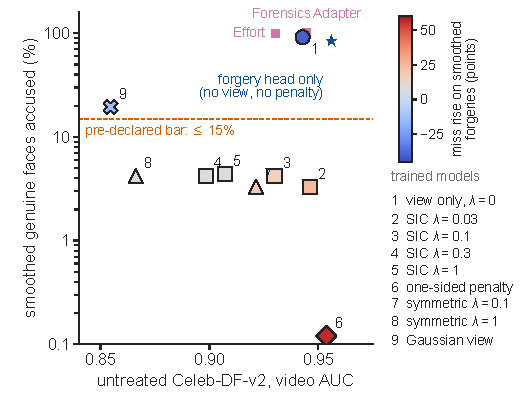
\includegraphics[width=3.5in]{fig_sic_curve_v8b}
\caption{The trade-off traced by the SIC family. Each point is one trained model: untreated Celeb-DF-v2 video AUC against
the share of skin-smoothed genuine faces accused (face-local 0.12, log scale); colour gives the rise of the miss rate on the
same smoothing applied to forgeries. The star is the model without the rule; squares are the published CLIP detectors. Every
penalty weight removes the accusation; smaller weights keep untreated detection and let more smoothed forgeries through.}
% figs/fig_sic_curve_v8b.pdf (make_fig_sic_curve_v8b.py from readout46.json, smooth38.json [clipe5b_s20260929].forms.fl12.fa,
% SMOOTH38.md, compare_sota_clipe5b_s20260929.json)
\label{fig:siccurve}
\end{figure}
The rule tested in Finding~6 of the paper follows from the exposure arms (Sec.~\ref{sec:chain}): for every training item $x$,
genuine, beautified or forged, a smoothed copy $x_s$ is drawn by one operator with one distribution of strengths, so that no
class can learn the form of the smoothing as a label, and the forged logit of the copy is asked not to move:
\begin{equation}
\mathcal{L}=\mathcal{L}_\text{BCE}\big(z_f(x),y\big)+\mathcal{L}_\text{map}+\lambda\,\big(\operatorname{sg}[z_f(x)]-z_f(x_s)\big)^2,
\label{eq:sic}
\end{equation}
where $\operatorname{sg}$ stops the gradient: the clean logit is the target, only the smoothed view is pulled, and the clean
path is trained by the classification loss alone. The map target of $x_s$ is the footprint of $x$. With the gradient through
both sides (the ``without stop-gradient'' rows of Table~\ref{tab:recal}) the clean forgery score of a forgery whose cue is
texture is pulled down toward its smoothed copy and untreated detection falls further. The operator is face-local bilateral
smoothing inside the landmark hull at a random strength, or whole-crop bilateral smoothing where no landmarks are carried; the
median filter, the Gaussian blend, the commercial renders and the AR renders are never used in training. The one-sided variant
penalises only a rise of the logit; the Gaussian ablation replaces the operator by a Gaussian blur of the same support.

\textbf{Bars.} Written before training (Addendum 46 and its amendments; READOUT46.md): (1) false alarms at most 15\% on the
face-local smoothed genuine Celeb-DF-v2 frames; (2) at most 15\% on the whole-crop bilateral forms and on the commercial
Smoothing-90 renders; (3) a miss rise on smoothed forgeries at most 5 points above the arm without views, as written, and
(3$'$) the relaxed form, at most $\max(\text{P0 rise},0)+5$; (4) untreated Celeb-DF-v2 and DFD video AUC not lower than the
model without the rule by more than 0.010; (5) Celeb-DF-B AUC under the presets not below the main model; (6) DF40 reenactment
video AUC not lower by more than 0.030; a $\lambda=0$ control; two seeds. Point estimates decide. Bar (3) as written is met by
no member; the ``passed'' count of Table~\ref{M-tab:sic} counts bars 1, 2, 3$'$, 4, 5 and 6.
\begin{table}[H]
\centering
\caption{Bars met by every trained member of the family (READOUT46.md). Bar numbers as in the text; ``passed'' counts bars 1,
2, 3$'$, 4, 5, 6.}
\label{tab:sicbars}
\scriptsize
\begin{adjustbox}{max width=\linewidth}% generated by make_tables_v8_supp.py from retouch_unified_20260929/READOUT46.md (bars lines)
\begin{tabular}{@{}l c ccccccc c@{}}
\toprule
Arm & seed & 1 face-local FA & 2 whole-crop and S-90 & 3 as written & 3$'$ relaxed & 4 untreated video & 5 Celeb-DF-B AUC & 6 DF40 reenactment & passed \\
\midrule
SIC factorised (primary) & 1 & \checkmark & \checkmark & -- & -- & -- & -- & -- & 2/6 \\
SIC binary (secondary) & 1 & \checkmark & \checkmark & -- & -- & -- & -- & -- & 2/6 \\
SIC binary (secondary) & 2 & \checkmark & \checkmark & -- & -- & -- & -- & -- & 2/6 \\
SIC binary, lambda 0 control & 1 & -- & \checkmark & -- & -- & -- & \checkmark & \checkmark & 3/6 \\
SIC binary, lambda 0.3 & 1 & \checkmark & \checkmark & -- & -- & -- & -- & -- & 2/6 \\
SIC binary, lambda 0.1 & 1 & \checkmark & \checkmark & -- & -- & -- & \checkmark & -- & 3/6 \\
SIC binary, stop-gradient & 1 & \checkmark & \checkmark & -- & -- & -- & -- & -- & 2/6 \\
SIC binary, stop-gradient & 2 & \checkmark & \checkmark & -- & -- & -- & -- & -- & 2/6 \\
FF++-only SIC binary, stop-gradient & 1 & \checkmark & \checkmark & -- & -- & -- & -- & -- & 2/6 \\
SIC-sg binary, lambda 0.3 & 1 & \checkmark & \checkmark & -- & -- & -- & -- & -- & 2/6 \\
SIC-sg binary, lambda 0.1 & 1 & \checkmark & \checkmark & -- & -- & -- & \checkmark & -- & 3/6 \\
SIC-sg binary, lambda 0.1 & 2 & \checkmark & \checkmark & -- & -- & -- & -- & -- & 2/6 \\
SIC-sg binary, Gaussian operator ablation & 1 & -- & \checkmark & -- & -- & -- & -- & -- & 1/6 \\
SIC-sg binary, Gaussian operator ablation & 2 & \checkmark & \checkmark & -- & -- & -- & -- & -- & 2/6 \\
SIC-h binary, one-sided consistency & 1 & \checkmark & \checkmark & -- & -- & \checkmark & \checkmark & -- & 4/6 \\
SIC-h binary, one-sided consistency & 2 & \checkmark & \checkmark & -- & -- & -- & -- & -- & 2/6 \\
SIC-sg binary, lambda 0.03 & 1 & \checkmark & \checkmark & -- & -- & \checkmark & \checkmark & -- & 4/6 \\
SIC-sg binary, lambda 0.03 & 2 & \checkmark & \checkmark & -- & -- & -- & -- & -- & 2/6 \\
\bottomrule
\end{tabular}
\end{adjustbox}
\end{table}
\begin{table}[H]
\centering
\caption{The full family, including the variants without the stop-gradient (symmetric penalty) and the FF++-only member.
Columns as in Table~\ref{M-tab:sic}.}
\label{tab:sicfull}
\scriptsize
\begin{adjustbox}{max width=\linewidth}\begin{tabular}{@{}lcccccccccccc@{}}
\toprule
Model & seed & \multicolumn{3}{c}{smoothed genuine accused (\%)} & S-90 & $\Delta$miss & \multicolumn{2}{c}{untreated video AUC} & Celeb-DF-B & DF40 FR & bars \\
 & & fl 0.06 & fl 0.12 & bil 15 & acc.\ \% & fl 0.12 & CDFv2 & DFD & AUC & ff & passed \\
\midrule
forgery head only, no rule & 1 & 51.6 & 84.5 & 35.5 & 9.1 & $-$34.0 & 0.956 & 0.987 & 0.866 & 0.842 & -- \\
\midrule
symmetric view only ($\lambda=0$) & 1 & 53.9 & 91.8 & 1.6 & 11.9 & $-$40.1 & 0.943 & 0.975 & 0.891 & 0.835 & 3/6 \\
SIC, $\lambda=0.03$ & 1 & 5.0 & 3.3 & 9.6 & 11.2 & 24.4 & 0.946 & 0.979 & 0.886 & 0.750 & 4/6 \\
SIC, $\lambda=0.03$ & 2 & 3.8 & 3.5 & 8.8 & 15.0 & 20.4 & 0.933 & 0.975 & 0.876 & 0.777 & 2/6 \\
SIC, $\lambda=0.1$ & 1 & 6.5 & 4.2 & 9.9 & 10.5 & 15.8 & 0.930 & 0.980 & 0.871 & 0.774 & 3/6 \\
SIC, $\lambda=0.1$ & 2 & 4.6 & 4.6 & 8.5 & 8.1 & 17.6 & 0.929 & 0.974 & 0.868 & 0.771 & 2/6 \\
SIC, $\lambda=0.3$ & 1 & 6.0 & 4.2 & 8.1 & 12.8 & 9.5 & 0.898 & 0.971 & 0.840 & 0.692 & 2/6 \\
SIC, $\lambda=1$ & 1 & 5.8 & 4.4 & 5.8 & 2.1 & 9.7 & 0.907 & 0.986 & 0.835 & 0.768 & 2/6 \\
SIC, $\lambda=1$ & 2 & 6.2 & 5.5 & 6.3 & 12.3 & 6.1 & 0.844 & 0.968 & 0.804 & 0.746 & 2/6 \\
one-sided penalty & 1 & 0.1 & 0.1 & 0.0 & 9.2 & 56.5 & 0.954 & 0.980 & 0.880 & 0.794 & 4/6 \\
one-sided penalty & 2 & 0.1 & 0.0 & 0.0 & 10.4 & 47.3 & 0.929 & 0.975 & 0.860 & 0.775 & 2/6 \\
Gaussian view (ablation) & 1 & 5.8 & 19.5 & 1.1 & 3.5 & $-$13.5 & 0.855 & 0.971 & 0.819 & 0.782 & 1/6 \\
Gaussian view (ablation) & 2 & 5.9 & 14.5 & 1.3 & 8.7 & $-$9.3 & 0.848 & 0.960 & 0.821 & 0.784 & 2/6 \\
SIC, $\lambda=1$, FF++ only & 1 & 7.4 & 6.8 & 5.3 & 7.0 & 4.8 & 0.856 & 0.979 & 0.829 & 0.674 & 2/6 \\
symmetric penalty, $\lambda=0.1$ & 1 & 4.3 & 3.3 & 7.1 & 9.5 & 18.6 & 0.921 & 0.974 & 0.882 & 0.760 & 3/6 \\
symmetric penalty, $\lambda=0.3$ & 1 & 4.7 & 4.6 & 8.1 & 9.9 & 12.4 & 0.900 & 0.966 & 0.860 & 0.755 & 2/6 \\
symmetric penalty, $\lambda=1$ & 1 & 4.9 & 4.2 & 7.0 & 7.1 & 7.8 & 0.866 & 0.956 & 0.837 & 0.702 & 2/6 \\
symmetric penalty, $\lambda=1$ & 2 & 4.7 & 5.3 & 6.9 & 7.6 & 6.3 & 0.858 & 0.955 & 0.829 & 0.712 & 2/6 \\
symmetric penalty, full model, $\lambda=1$ & 1 & 4.5 & 4.3 & 7.2 & 7.6 & 10.2 & 0.876 & 0.968 & 0.845 & 0.663 & 2/6 \\
smoothing expert (trained on smoothed copies only; routed model B) & 1 & 10.8 & 16.4 & 93.5 & 12.5 & $-$11.2 & 0.904 & 0.978 & 0.836 & 0.529 & 0/6 \\
smoothing expert (trained on smoothed copies only; routed model B) & 2 & 11.7 & 13.6 & 76.6 & 12.8 & $-$6.3 & 0.880 & -- & -- & 0.468 & 2/4 \\
FF++-only P0 without Deepfakes and NeuralTextures & 1 & 95.5 & 100.0 & 17.1 & 33.5 & $-$45.0 & 0.918 & 0.984 & 0.868 & 0.631 & 2/6 \\
\bottomrule
\end{tabular}
\end{adjustbox}
\end{table}

\textbf{Recalibration control.} Table~\ref{tab:recal} reads every model with both classes smoothed by the same form and the
threshold re-set at 5\% FPR on the smoothed genuine frames of that form (an oracle): the cell is the AUC between smoothed
genuine and smoothed forged frames and the miss rate at that threshold. The $\lambda=0$ model (symmetric view, no penalty)
read this way has a both-classes-smoothed AUC of 0.832 and 0.764 (bilateral 15, face-local 0.12) against 0.790 and 0.778 for
SIC at $\lambda=1$ and 0.802 and 0.778 at $\lambda=0.1$, and a recalibrated miss of 57.4 and 76.7\% against 64--73\% for SIC on
two seeds; this is the basis of the paper's reading of SIC as a smoothing-conditional recalibration. Every published detector
loses AUC with both classes smoothed (0.06--0.28 at face-local 0.12 for the sixteen above chance), and the $\lambda=0$ model
loses 0.061 and 0.129 from its untreated 0.893.
\begin{table}[H]
\centering
\caption{Both classes smoothed, threshold re-set at 5\% FPR on the same condition's genuine frames (oracle recalibration). Cell:
AUC / miss rate (\%). Celeb-DF-v2 test, frames with landmarks (RECAL\_MISS.md).}
\label{tab:recal}
\scriptsize
\begin{adjustbox}{max width=\linewidth}% generated by make_tables_v8_supp.py from retouch_unified_20260929/RECAL_MISS.md
\begin{tabular}{@{}l ccccc@{}}
\toprule
Model & untreated & bilateral 15 & bilateral 21 & face-local 0.06 & face-local 0.12 \\
\midrule
\oursB{}, seed 1 & 0.909 / 36.5 & 0.805 / 63.1 & 0.754 / 67.8 & 0.886 / 47.0 & 0.755 / 73.7 \\
\oursB{}, seed 2 & 0.917 / 35.4 & 0.843 / 52.0 & 0.810 / 59.0 & 0.879 / 48.8 & 0.748 / 75.4 \\
symmetric view only ($\lambda=0$) & 0.893 / 40.7 & 0.832 / 57.4 & 0.798 / 64.5 & 0.870 / 53.2 & 0.764 / 76.7 \\
SIC without stop-gradient, $\lambda=1$, seed 1 & 0.813 / 62.9 & 0.756 / 69.1 & 0.752 / 70.7 & 0.790 / 64.9 & 0.749 / 68.9 \\
SIC without stop-gradient, $\lambda=1$, seed 2 & 0.805 / 65.2 & 0.751 / 71.6 & 0.742 / 71.8 & 0.783 / 66.0 & 0.733 / 72.6 \\
SIC, $\lambda=1$, seed 1 & 0.841 / 55.5 & 0.790 / 64.5 & 0.791 / 63.6 & 0.825 / 58.0 & 0.778 / 64.0 \\
SIC, $\lambda=1$, seed 2 & 0.782 / 66.0 & 0.733 / 73.0 & 0.731 / 73.5 & 0.769 / 69.1 & 0.720 / 72.8 \\
SIC, $\lambda=0.3$ & 0.829 / 59.1 & 0.765 / 68.5 & 0.756 / 71.7 & 0.819 / 59.3 & 0.759 / 66.4 \\
SIC, $\lambda=0.1$ & 0.864 / 47.6 & 0.802 / 62.8 & 0.795 / 61.3 & 0.841 / 53.5 & 0.778 / 61.0 \\
one-sided penalty, seed 1 & 0.892 / 42.9 & 0.727 / 71.9 & 0.691 / 76.4 & 0.667 / 71.9 & 0.603 / 77.4 \\
one-sided penalty, seed 2 & 0.862 / 52.3 & 0.738 / 72.6 & 0.714 / 76.0 & 0.654 / 77.7 & 0.606 / 81.5 \\
Gaussian view (ablation) & 0.802 / 65.4 & 0.703 / 75.6 & 0.694 / 77.3 & 0.760 / 69.1 & 0.705 / 72.6 \\
Xception & 0.717 / 77.7 & 0.544 / 93.3 & 0.487 / 96.1 & 0.669 / 83.8 & 0.580 / 90.7 \\
EfficientNet-B4 & 0.746 / 76.7 & 0.590 / 95.2 & 0.553 / 94.9 & 0.679 / 90.7 & 0.531 / 97.0 \\
F3Net & 0.712 / 82.0 & 0.611 / 92.4 & 0.577 / 94.2 & 0.697 / 85.6 & 0.652 / 95.5 \\
SPSL & 0.703 / 79.3 & 0.561 / 92.2 & 0.533 / 92.1 & 0.652 / 83.2 & 0.631 / 84.2 \\
UCF & 0.742 / 74.2 & 0.490 / 95.4 & 0.423 / 96.1 & 0.673 / 89.6 & 0.535 / 94.8 \\
RECCE & 0.689 / 84.6 & 0.552 / 95.2 & 0.545 / 95.4 & 0.688 / 84.7 & 0.607 / 92.0 \\
CORE & 0.720 / 82.3 & 0.576 / 91.3 & 0.596 / 93.0 & 0.678 / 82.9 & 0.646 / 100.0 \\
SRM & 0.719 / 83.7 & 0.486 / 97.4 & 0.504 / 96.4 & 0.590 / 92.9 & 0.513 / 94.7 \\
SBI & 0.815 / 62.3 & 0.644 / 88.5 & 0.531 / 94.6 & 0.660 / 89.9 & 0.577 / 93.4 \\
LAA-Net & 0.847 / 56.1 & 0.651 / 84.9 & 0.582 / 90.3 & 0.603 / 89.5 & 0.566 / 92.3 \\
CADDM & 0.832 / 57.3 & 0.610 / 90.9 & 0.590 / 93.1 & 0.733 / 74.9 & 0.572 / 91.7 \\
Effort & 0.876 / 41.3 & 0.785 / 67.7 & 0.748 / 76.6 & 0.749 / 81.1 & 0.658 / 84.0 \\
Forensics Adapter & 0.883 / 42.9 & 0.705 / 82.5 & 0.668 / 87.6 & 0.705 / 82.3 & 0.649 / 87.6 \\
GenD & 0.887 / 39.9 & 0.771 / 80.1 & 0.712 / 83.5 & 0.677 / 90.9 & 0.632 / 90.8 \\
DFD-HR & 0.869 / 45.7 & 0.751 / 72.0 & 0.713 / 75.5 & 0.701 / 86.5 & 0.601 / 93.5 \\
UnivFD & 0.663 / 83.4 & 0.524 / 94.9 & 0.511 / 96.0 & 0.689 / 83.5 & 0.579 / 97.6 \\
NPR & 0.527 / 93.6 & 0.500 / 100.0 & 0.500 / 100.0 & 0.538 / 100.0 & 0.521 / 100.0 \\
\bottomrule
\end{tabular}
\end{adjustbox}
\end{table}

\textbf{Routed expert.} A second model B trained only on smoothed copies ($x_s$ of every class) is selected by the smoothing
score $p_s$ of the three-way model (route to B when $p_s$ exceeds the FF++-validation threshold); A is the forgery-head-only
model of the same seed. Table~\ref{tab:sce} gives seed 20260930, the only seed read so far. Routing clears the accusation on
the face-local forms (51.2 and 79.9\% to 2.1 and 1.3\%), raises the miss on the same smoothed forgeries by 40.6 and 46.0
points, and B's both-classes-smoothed AUC is below A's on seven of the eight forms. On the commercial renders the routed
decision accuses 0.2\% of Smoothing-90 renders (A: 6.5\%) and 4.8\% of the originals; 99.4\% of the renders and 0.9\% of the
originals are routed.
\begin{table}[H]
\centering
\caption{Routed expert (SCE), seed 20260930. Share of frames routed to the smoothing expert B, false alarms and misses of A
alone and of the routed decision at the 5\%-FPR rule, and the AUC with both classes smoothed of A and of B (SCE\_s2.md).}
\label{tab:sce}
\scriptsize
\begin{adjustbox}{max width=\linewidth}% generated by make_tables_v8_supp.py from retouch_unified_20260929/SCE_s2.md (seed 20260930)
\begin{tabular}{@{}l c c c c c@{}}
\toprule
Form & routed to B (\%) & FA, A $\rightarrow$ routed [CI] & MISS, A $\rightarrow$ routed & miss rise, A $\rightarrow$ routed & AUC both smoothed, A / B \\
\midrule
untreated & 0.0 & 5.0 $\rightarrow$ 5.0 [3.7, 6.2] & 35.4 $\rightarrow$ 35.4 & 0.0 $\rightarrow$ 0.0 & 0.917 / 0.8129 \\
bil9 & 99.9 & 2.2 $\rightarrow$ 6.8 [4.6, 8.3] & 57.8 $\rightarrow$ 56.7 & 22.4 $\rightarrow$ 21.3 & 0.8785 / 0.8014 \\
bil15 & 100.0 & 9.3 $\rightarrow$ 7.8 [5.8, 9.6] & 41.7 $\rightarrow$ 65.3 & 6.3 $\rightarrow$ 29.8 & 0.843 / 0.7518 \\
bil21 & 100.0 & 17.2 $\rightarrow$ 6.2 [4.5, 7.7] & 37.6 $\rightarrow$ 69.2 & 2.2 $\rightarrow$ 33.7 & 0.81 / 0.7443 \\
median5 & 74.4 & 3.4 $\rightarrow$ 5.5 [3.9, 7.0] & 49.0 $\rightarrow$ 56.8 & 13.6 $\rightarrow$ 21.4 & 0.8825 / 0.7511 \\
gblend & 3.6 & 3.6 $\rightarrow$ 3.4 [2.3, 4.5] & 43.7 $\rightarrow$ 46.0 & 8.4 $\rightarrow$ 10.6 & 0.8996 / 0.8009 \\
fl06 & 99.8 & 51.2 $\rightarrow$ 2.1 [0.8, 3.0] & 4.6 $\rightarrow$ 76.0 & $-$30.8 $\rightarrow$ 40.6 & 0.879 / 0.816 \\
fl12 & 100.0 & 79.9 $\rightarrow$ 1.3 [0.5, 2.0] & 3.2 $\rightarrow$ 81.4 & $-$32.2 $\rightarrow$ 46.0 & 0.7484 / 0.7697 \\
\bottomrule
\end{tabular}
\end{adjustbox}
\end{table}

\section{A smoothing-conditional threshold, every detector}
\label{sec:bct}
Table~\ref{tab:bct} gives the rule of Finding~5 (Table~\ref{M-tab:bct}) for every detector: fake iff $s>t_0+\Delta(b)$, with
$t_0$ the 95th percentile of untreated genuine frames and $\Delta$ learnt on FF++ validation genuine renders only, binned by the
skin-smoothing presence probability $b$ of the three-way model (bins at 0.1, 0.5, 0.9). Cells read fixed $\rightarrow$
conditional. The last column is the shift learnt for the top bin. The rule lowers the accusation of smoothed genuine faces for
every detector that is sensitive to $b$ and raises the miss on smoothed forgeries by the same mechanism; NPR, whose scores
saturate, is unchanged.
\begin{table}[H]
\centering
\caption{Beautification-conditional threshold (BCT, Addendum 47) for every detector. FA on untreated, face-local 0.06 / 0.12
and bilateral 15 smoothed genuine Celeb-DF-v2 frames and on the commercial Smoothing-90 renders; MISS on face-local 0.12 and
bilateral 15 smoothed forgeries and on untreated forgeries (\%), fixed $\rightarrow$ conditional (BCT.md).}
\label{tab:bct}
\scriptsize
\begin{adjustbox}{max width=\linewidth}% generated by make_tables_v8_supp.py from retouch_unified_20260929/BCT.md (Addendum 47)
\begin{tabular}{@{}l ccccc ccc c@{}}
\toprule
Detector & untreated FA & fl 0.06 FA & fl 0.12 FA & bil 15 FA & S-90 accused & fl 0.12 MISS & bil 15 MISS & untreated MISS & $\Delta$ (top bin) \\
\midrule
Xception & 5.0 $\rightarrow$ 5.0 & 89.2 $\rightarrow$ 64.4 & 99.3 $\rightarrow$ 92.4 & 76.7 $\rightarrow$ 22.4 & 51.6 $\rightarrow$ 0.0 & 0.2 $\rightarrow$ 4.2 & 18.1 $\rightarrow$ 72.7 & 77.7 $\rightarrow$ 79.1 & 0.1308 \\
EfficientNet-B4 & 5.0 $\rightarrow$ 5.0 & 64.3 $\rightarrow$ 51.5 & 95.0 $\rightarrow$ 90.4 & 79.7 $\rightarrow$ 67.8 & 36.3 $\rightarrow$ 0.0 & 1.1 $\rightarrow$ 2.9 & 9.1 $\rightarrow$ 20.4 & 76.7 $\rightarrow$ 77.3 & 0.077 \\
F3Net & 5.0 $\rightarrow$ 5.0 & 86.3 $\rightarrow$ 81.0 & 99.6 $\rightarrow$ 99.3 & 98.5 $\rightarrow$ 94.6 & 50.6 $\rightarrow$ 0.0 & 0.0 $\rightarrow$ 0.0 & 0.1 $\rightarrow$ 0.7 & 82.0 $\rightarrow$ 82.9 & 0.0753 \\
SPSL & 5.0 $\rightarrow$ 5.0 & 70.3 $\rightarrow$ 28.4 & 92.1 $\rightarrow$ 65.5 & 63.1 $\rightarrow$ 8.4 & 51.2 $\rightarrow$ 0.9 & 3.6 $\rightarrow$ 19.6 & 29.9 $\rightarrow$ 86.8 & 79.3 $\rightarrow$ 80.4 & 0.0551 \\
UCF & 5.0 $\rightarrow$ 5.0 & 89.3 $\rightarrow$ 88.8 & 98.4 $\rightarrow$ 98.0 & 24.3 $\rightarrow$ 22.6 & 41.4 $\rightarrow$ 0.0 & 0.5 $\rightarrow$ 0.8 & 77.5 $\rightarrow$ 79.2 & 74.2 $\rightarrow$ 74.3 & 0.0066 \\
RECCE & 5.0 $\rightarrow$ 5.0 & 80.7 $\rightarrow$ 22.7 & 97.8 $\rightarrow$ 45.3 & 91.8 $\rightarrow$ 2.0 & 36.8 $\rightarrow$ 0.0 & 0.5 $\rightarrow$ 39.7 & 3.4 $\rightarrow$ 97.5 & 84.6 $\rightarrow$ 86.1 & 0.0582 \\
CORE & 5.0 $\rightarrow$ 5.0 & 85.0 $\rightarrow$ 53.2 & 99.7 $\rightarrow$ 97.6 & 99.3 $\rightarrow$ 88.4 & 54.8 $\rightarrow$ 0.0 & 0.1 $\rightarrow$ 0.8 & 0.1 $\rightarrow$ 3.8 & 82.3 $\rightarrow$ 84.1 & 0.1464 \\
SRM & 5.0 $\rightarrow$ 5.0 & 81.0 $\rightarrow$ 12.8 & 91.8 $\rightarrow$ 9.4 & 74.0 $\rightarrow$ 5.4 & 62.8 $\rightarrow$ 17.3 & 5.7 $\rightarrow$ 90.9 & 25.8 $\rightarrow$ 97.1 & 83.7 $\rightarrow$ 84.8 & 0.0808 \\
SBI & 5.0 $\rightarrow$ 5.0 & 96.7 $\rightarrow$ 0.0 & 100.0 $\rightarrow$ 0.0 & 72.3 $\rightarrow$ 0.0 & 37.3 $\rightarrow$ 0.0 & 0.0 $\rightarrow$ 100.0 & 10.7 $\rightarrow$ 100.0 & 62.3 $\rightarrow$ 66.4 & 0.2027 \\
UnivFD & 5.0 $\rightarrow$ 5.0 & 13.9 $\rightarrow$ 0.9 & 55.2 $\rightarrow$ 11.1 & 40.8 $\rightarrow$ 5.8 & 16.6 $\rightarrow$ 1.0 & 28.8 $\rightarrow$ 90.8 & 56.1 $\rightarrow$ 93.8 & 83.4 $\rightarrow$ 83.5 & 0.7776 \\
NPR & 5.0 $\rightarrow$ 5.0 & 68.0 $\rightarrow$ 68.0 & 77.7 $\rightarrow$ 77.7 & 100.0 $\rightarrow$ 100.0 & 0.0 $\rightarrow$ 0.0 & 18.7 $\rightarrow$ 18.7 & 0.0 $\rightarrow$ 0.0 & 93.6 $\rightarrow$ 93.6 & 0.0 \\
Effort & 5.0 $\rightarrow$ 4.9 & 87.8 $\rightarrow$ 0.0 & 99.9 $\rightarrow$ 0.0 & 27.1 $\rightarrow$ 0.0 & 43.2 $\rightarrow$ 20.5 & 0.0 $\rightarrow$ 100.0 & 32.2 $\rightarrow$ 100.0 & 41.3 $\rightarrow$ 47.0 & 0.2118 \\
Forensics Adapter & 5.0 $\rightarrow$ 4.9 & 95.8 $\rightarrow$ 0.1 & 100.0 $\rightarrow$ 0.0 & 59.9 $\rightarrow$ 0.0 & 39.7 $\rightarrow$ 31.4 & 0.0 $\rightarrow$ 100.0 & 13.3 $\rightarrow$ 100.0 & 42.9 $\rightarrow$ 48.7 & 0.1975 \\
GenD & 5.0 $\rightarrow$ 5.0 & 96.1 $\rightarrow$ 3.9 & 100.0 $\rightarrow$ 11.7 & 81.7 $\rightarrow$ 0.6 & 68.7 $\rightarrow$ 32.4 & 0.0 $\rightarrow$ 78.3 & 1.5 $\rightarrow$ 93.7 & 39.9 $\rightarrow$ 42.9 & 0.1187 \\
DFD-HR & 5.0 $\rightarrow$ 5.0 & 99.3 $\rightarrow$ 0.4 & 100.0 $\rightarrow$ 0.6 & 79.8 $\rightarrow$ 0.0 & 64.9 $\rightarrow$ 36.8 & 0.0 $\rightarrow$ 99.3 & 4.4 $\rightarrow$ 100.0 & 45.7 $\rightarrow$ 47.6 & 0.3084 \\
CADDM & 5.0 $\rightarrow$ 5.0 & 88.5 $\rightarrow$ 0.0 & 99.9 $\rightarrow$ 0.0 & 61.4 $\rightarrow$ 0.0 & 6.3 $\rightarrow$ 0.0 & 0.0 $\rightarrow$ 100.0 & 24.3 $\rightarrow$ 100.0 & 57.3 $\rightarrow$ 60.6 & 0.1479 \\
LAA-Net & 5.0 $\rightarrow$ 4.8 & 100.0 $\rightarrow$ 98.8 & 100.0 $\rightarrow$ 100.0 & 92.1 $\rightarrow$ 61.1 & 17.2 $\rightarrow$ 0.0 & 0.0 $\rightarrow$ 0.0 & 1.6 $\rightarrow$ 20.9 & 56.1 $\rightarrow$ 57.8 & 0.1241 \\
\oursB{} & 5.0 $\rightarrow$ 5.0 & 51.6 $\rightarrow$ 0.0 & 84.5 $\rightarrow$ 0.1 & 35.5 $\rightarrow$ 0.0 & 9.1 $\rightarrow$ 4.9 & 2.5 $\rightarrow$ 100.0 & 21.0 $\rightarrow$ 100.0 & 36.5 $\rightarrow$ 36.5 & 0.0125 \\
\ours{} (three-way) & 5.0 $\rightarrow$ 4.8 & 5.8 $\rightarrow$ 0.0 & 44.5 $\rightarrow$ 0.0 & 79.8 $\rightarrow$ 0.0 & 8.6 $\rightarrow$ 0.9 & 32.9 $\rightarrow$ 100.0 & 4.7 $\rightarrow$ 100.0 & 47.0 $\rightarrow$ 53.2 & 0.3299 \\
SIC, $\lambda=1$ & 5.0 $\rightarrow$ 5.0 & 5.8 $\rightarrow$ 4.2 & 4.4 $\rightarrow$ 3.0 & 5.8 $\rightarrow$ 3.9 & 2.1 $\rightarrow$ 0.7 & 65.3 $\rightarrow$ 69.6 & 61.2 $\rightarrow$ 68.1 & 55.5 $\rightarrow$ 55.6 & 0.0849 \\
SIC, $\lambda=0.1$ & 5.0 $\rightarrow$ 5.0 & 6.5 $\rightarrow$ 0.0 & 4.2 $\rightarrow$ 0.0 & 9.9 $\rightarrow$ 0.0 & 10.5 $\rightarrow$ 3.3 & 63.4 $\rightarrow$ 99.9 & 51.4 $\rightarrow$ 100.0 & 47.6 $\rightarrow$ 47.9 & 0.0572 \\
\bottomrule
\end{tabular}
\end{adjustbox}
\end{table}

\section{The face against its context, and a test-time rule that does not work}
\label{sec:supp_context}
The band-energy analysis of the main text says that the cue is face-local and edge-preserving. A second probe asks whether the
cue is the line where the smoothed face meets the untouched background. Pre-registered on 2026-10-23 (Addendum 57), the same
bilateral strength is applied to Celeb-DF-B genuine frames in four face-local forms whose only difference is the edge treatment
(hard edge, then feathered over 1, 5 and 15 px), to the whole crop, and to a 12-px ring at the face edge alone, with the face
interior untouched. Every detector keeps its own threshold, set at 5\% false alarms on the untreated frames.
Fig.~\ref{fig:supp_context} gives the three forms that decide the question. The ring alone accuses 7--13\% of the frames for
fifteen of the seventeen published detectors, against 92--100\% for the face-local form (prediction ``ring reaches 70\% of
face-local'' holds for 1 of 15 face detectors, bar 10 of 15). Feathering the edge lowers the accusation monotonically for 14 of
15, so the edge contributes, but it is not the cue. Smoothing the whole crop accuses less than smoothing the face alone for 11 of
15 (by 10 points or more), so the detectors read a face that is smoother than its surroundings. CADDM (ring 94\%) and LAA-Net
(ring 65\%) are the two detectors that read the edge; both are trained on blending boundaries. Our three-way model runs the
other way (face-local 45\%, whole crop 81\%): it has seen whole-crop smoothing of genuine frames in training as a beautified
view and reads it as a class cue, the shortcut described in Sec.~\ref{sec:chain}.

This mechanism suggests a zero-training rule: score the image and a whole-crop-smoothed copy of it, and call the image forged
only if both exceed their thresholds, since the copy removes the face-context contrast of a beautified genuine face while a
forgery should keep evidence that does not depend on it. Pre-registered on 2026-10-27 (Addendum 61) with two predictions. The
first holds at its bar: the joint rule accuses fewer than 30\% of face-locally smoothed genuine frames for 10 of 15 face
detectors (single score: 92--100\%). The second, which decides whether the rule is more than a threshold, fails for every
detector: at a matched 5\% false-alarm rate on the same smoothed genuine frames, the joint rule misses smoothed forgeries within
a few points of the recalibrated single score (Effort 86.5 vs 84.0\%, Forensics Adapter 89.2 vs 87.6, GenD 90.2 vs 90.8, DFD-HR
90.7 vs 93.5, Xception 93.8 vs 90.7; 0 of 15 better by 10 points, kill bar 5 of 15), and the second gate raises the miss rate on
untreated forgeries by 20 to 35 points (Effort 41 to 77\%, SBI 62 to 96\%). Once a smoothed genuine face and a smoothed forgery
both pass the first threshold, the score on the context-matched copy carries no further separation between them. This is the
fourth independent closure of the same bound (threshold, routing, consistency training, context matching).

\begin{figure}[H]
\centering
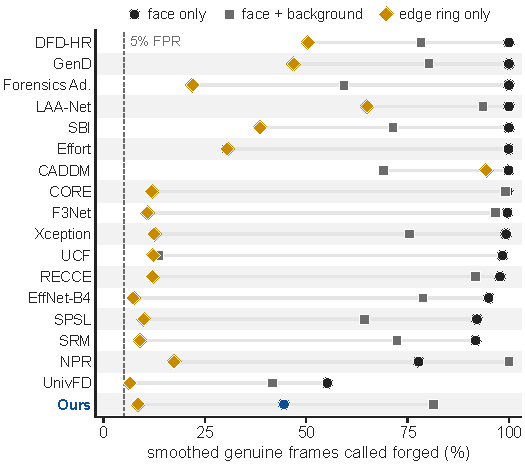
\includegraphics[width=3.5in]{fig_context_v8b}
\caption{Smoothed genuine Celeb-DF-B frames called forged at each detector's own 5\% FPR threshold, with the same bilateral
strength applied to the face only, to the whole crop, and to a 12-px ring at the face edge. Rows sorted by the face-only
share. The ring alone accuses almost nothing except for CADDM and LAA-Net; the whole crop accuses less than the face alone for
most detectors and more for ours.}
\label{fig:supp_context}
\end{figure}

\section{Identity as a reference channel}
\label{sec:idref}
The probes are the Celeb-DF-v2 test frames of Sec.~\ref{sec:smooth38} restricted to Celeb-real and Celeb-synthesis (3,504
frames: 836 genuine, 2,668 forged), untreated and under four smoothing forms; face detection fails on none. The identity score
is the ArcFace distance between the probe and a reference set of the claimed person's other videos (54 identities, 1,080
frames, none from the test videos). Intervals are bootstraps over claimed identities of the AUC change against untreated.
Table~\ref{tab:idref} gives the AUC and the error rates at the untreated 5\%-FPR threshold held fixed; the fusion row (mean
of the two quantile scores) is dominated by the identity distance alone at every condition and is not reported as a method in
the paper. Table~\ref{tab:ict} gives ICT and ICT-Ref~\cite{ict2022} on the same probes with the released weights: the main
ICT-Ref row uses our reference set through ICT's own alignment and $k=1$ nearest neighbour over the pool, as in the released
evaluation; the released reference file (2,420 entries of unknown provenance) and a claimed-identity pool are listed as
secondary readings. Their AUC falls by 0.08--0.12 under the three stronger forms with intervals wholly below $-0.05$, and
their failure direction is the opposite of the texture detectors': the forged median score falls, misses rise and the false
alarm does not. ID-Reveal was not run, because its temporal network reads 3DMM coefficients of consecutive frames that our
per-frame probes do not provide.
\begin{table}[H]
\centering
\caption{Identity distance against texture detectors on the same probes (ID\_REF.md, Addendum 51). Top: AUC, with the 95\%
identity-bootstrap interval of the change against untreated. Bottom: false alarm / miss (\%) at the untreated 5\%-FPR threshold.}
\label{tab:idref}
\scriptsize
\begin{adjustbox}{max width=\linewidth}% generated by make_tables_v8_supp.py from retouch_unified_20260929/ID_REF.md (Addendum 51, AUC table)
\begin{tabular}{@{}l ccccc@{}}
\toprule
Score & untreated & bilateral 15 & bilateral 21 & face-local 0.06 & face-local 0.12 \\
\midrule
identity (ArcFace distance) & 0.9962 & 0.9839 [$-$0.0219, $-$0.0053] & 0.9629 [$-$0.0545, $-$0.0166] & 0.9946 [$-$0.0034, $-$0.0003] & 0.9815 [$-$0.0264, $-$0.0053] \\
\oursB{} & 0.9244 & 0.8229 [$-$0.1238, $-$0.0812] & 0.7776 [$-$0.1755, $-$0.1199] & 0.8869 [$-$0.0686, $-$0.0105] & 0.7507 [$-$0.2135, $-$0.135] \\
Effort & 0.8966 & 0.8124 [$-$0.1085, $-$0.0588] & 0.7795 [$-$0.1476, $-$0.0862] & 0.7626 [$-$0.1824, $-$0.0968] & 0.663 [$-$0.2843, $-$0.1912] \\
GenD & 0.904 & 0.8042 [$-$0.1348, $-$0.0646] & 0.7343 [$-$0.2101, $-$0.1273] & 0.6645 [$-$0.2918, $-$0.1872] & 0.6055 [$-$0.3478, $-$0.2477] \\
SBI & 0.8323 & 0.6997 [$-$0.1831, $-$0.0918] & 0.5764 [$-$0.3161, $-$0.2004] & 0.6376 [$-$0.2623, $-$0.1345] & 0.5726 [$-$0.3371, $-$0.1948] \\
fusion \oursB{} + identity & 0.9895 & 0.9572 [$-$0.0454, $-$0.0206] & 0.9343 [$-$0.0751, $-$0.0379] & 0.9828 [$-$0.0149, 0.0005] & 0.943 [$-$0.0637, $-$0.0322] \\
\bottomrule
\end{tabular}
\end{adjustbox}\\[4pt]
\begin{adjustbox}{max width=\linewidth}% generated by make_tables_v8_supp.py from retouch_unified_20260929/ID_REF.md (Addendum 51, FA / miss table)
\begin{tabular}{@{}l ccccc@{}}
\toprule
Score & untreated & bilateral 15 & bilateral 21 & face-local 0.06 & face-local 0.12 \\
\midrule
identity (ArcFace distance) & 5.0 / 0.1 & 19.4 / 0.1 & 40.0 / 0.0 & 6.3 / 0.2 & 21.3 / 0.3 \\
\oursB{} & 5.0 / 33.8 & 43.2 / 14.4 & 53.5 / 14.9 & 56.6 / 3.8 & 88.0 / 1.8 \\
Effort & 5.0 / 33.4 & 41.5 / 16.8 & 66.5 / 5.3 & 94.9 / 0.1 & 100.0 / 0.0 \\
GenD & 5.0 / 30.6 & 88.0 / 0.6 & 96.8 / 0.1 & 98.8 / 0.0 & 100.0 / 0.0 \\
SBI & 5.0 / 55.0 & 74.2 / 5.7 & 92.6 / 1.2 & 98.2 / 0.1 & 100.0 / 0.0 \\
fusion \oursB{} + identity & 5.0 / 5.7 & 14.8 / 9.4 & 20.6 / 10.9 & 7.8 / 6.0 & 22.6 / 8.7 \\
\bottomrule
\end{tabular}
\end{adjustbox}
\end{table}
\begin{table}[H]
\centering
\caption{ICT and ICT-Ref with released weights on the same probes (ICT\_PROBE.md, Addendum 52). Top: AUC, change against
untreated in parentheses, with its 95\% identity-bootstrap interval. Bottom: false alarm / miss (\%) at the untreated 5\%-FPR
threshold.}
\label{tab:ict}
\scriptsize
\begin{adjustbox}{max width=\linewidth}% generated by make_tables_v8_supp.py from retouch_unified_20260929/ICT_PROBE.md (Addendum 52, AUC table)
\begin{tabular}{@{}l ccccc@{}}
\toprule
Score & untreated & bilateral 15 & bilateral 21 & face-local 0.06 & face-local 0.12 \\
\midrule
ICT & 0.7898 & 0.6789 ($-$0.1109) [$-$0.1457, $-$0.0806] & 0.6664 ($-$0.1234) [$-$0.1695, $-$0.0831] & 0.7518 ($-$0.0380) [$-$0.0513, $-$0.0259] & 0.6983 ($-$0.0915) [$-$0.126, $-$0.0604] \\
ICT-Ref (our reference set) & 0.863 & 0.7811 ($-$0.0819) [$-$0.1068, $-$0.0599] & 0.7546 ($-$0.1084) [$-$0.1462, $-$0.0686] & 0.8355 ($-$0.0276) [$-$0.0364, $-$0.0197] & 0.7828 ($-$0.0803) [$-$0.102, $-$0.0568] \\
ICT-Ref (released reference) & 0.9325 & 0.8804 ($-$0.0521) [$-$0.0684, $-$0.0362] & 0.8402 ($-$0.0923) [$-$0.119, $-$0.0649] & 0.9189 ($-$0.0136) [$-$0.019, $-$0.0079] & 0.8881 ($-$0.0444) [$-$0.0604, $-$0.0275] \\
ICT-Ref (claimed-identity reference) & 0.793 & 0.7111 ($-$0.0819) [$-$0.1118, $-$0.0558] & 0.7024 ($-$0.0906) [$-$0.1318, $-$0.0501] & 0.7617 ($-$0.0313) [$-$0.0399, $-$0.0227] & 0.7133 ($-$0.0797) [$-$0.1082, $-$0.0532] \\
identity (ArcFace distance) & 0.9962 & 0.9839 ($-$0.0123) [$-$0.0219, $-$0.0053] & 0.9629 ($-$0.0333) [$-$0.0545, $-$0.0166] & 0.9946 ($-$0.0015) [$-$0.0034, $-$0.0003] & 0.9815 ($-$0.0147) [$-$0.0264, $-$0.0053] \\
\oursB{} & 0.9244 & 0.8229 ($-$0.1016) [$-$0.1238, $-$0.0812] & 0.7776 ($-$0.1468) [$-$0.1755, $-$0.1199] & 0.8869 ($-$0.0376) [$-$0.0686, $-$0.0105] & 0.7507 ($-$0.1737) [$-$0.2135, $-$0.135] \\
Effort & 0.8966 & 0.8124 ($-$0.0841) [$-$0.1085, $-$0.0588] & 0.7795 ($-$0.1170) [$-$0.1476, $-$0.0862] & 0.7626 ($-$0.1339) [$-$0.1824, $-$0.0968] & 0.663 ($-$0.2335) [$-$0.2843, $-$0.1912] \\
GenD & 0.904 & 0.8042 ($-$0.0997) [$-$0.1348, $-$0.0646] & 0.7343 ($-$0.1697) [$-$0.2101, $-$0.1273] & 0.6645 ($-$0.2395) [$-$0.2918, $-$0.1872] & 0.6055 ($-$0.2985) [$-$0.3478, $-$0.2477] \\
SBI & 0.8323 & 0.6997 ($-$0.1326) [$-$0.1831, $-$0.0918] & 0.5764 ($-$0.2559) [$-$0.3161, $-$0.2004] & 0.6376 ($-$0.1947) [$-$0.2623, $-$0.1345] & 0.5726 ($-$0.2597) [$-$0.3371, $-$0.1948] \\
\bottomrule
\end{tabular}
\end{adjustbox}\\[4pt]
\begin{adjustbox}{max width=\linewidth}% generated by make_tables_v8_supp.py from retouch_unified_20260929/ICT_PROBE.md (Addendum 52, FA / miss table)
\begin{tabular}{@{}l ccccc@{}}
\toprule
Score & untreated & bilateral 15 & bilateral 21 & face-local 0.06 & face-local 0.12 \\
\midrule
ICT & 5.0 / 65.3 & 2.3 / 87.8 & 2.5 / 85.3 & 3.7 / 73.3 & 4.7 / 75.7 \\
ICT-Ref (our reference set) & 5.0 / 46.6 & 2.9 / 70.4 & 7.2 / 64.1 & 4.1 / 54.6 & 5.5 / 56.5 \\
ICT-Ref (released reference) & 5.0 / 32.3 & 4.7 / 52.7 & 12.3 / 39.8 & 4.9 / 40.0 & 7.1 / 39.1 \\
ICT-Ref (claimed-identity reference) & 5.0 / 62.9 & 3.1 / 80.8 & 5.4 / 72.5 & 4.3 / 69.8 & 5.4 / 69.5 \\
identity (ArcFace distance) & 5.0 / 0.1 & 19.4 / 0.1 & 40.0 / 0.0 & 6.3 / 0.2 & 21.3 / 0.3 \\
\oursB{} & 5.0 / 33.8 & 43.2 / 14.4 & 53.5 / 14.9 & 56.6 / 3.8 & 88.0 / 1.8 \\
Effort & 5.0 / 33.4 & 41.5 / 16.8 & 66.5 / 5.3 & 94.9 / 0.1 & 100.0 / 0.0 \\
GenD & 5.0 / 30.6 & 88.0 / 0.6 & 96.8 / 0.1 & 98.8 / 0.0 & 100.0 / 0.0 \\
SBI & 5.0 / 55.0 & 74.2 / 5.7 & 92.6 / 1.2 & 98.2 / 0.1 & 100.0 / 0.0 \\
\bottomrule
\end{tabular}
\end{adjustbox}
\end{table}

\section{Second seeds of the variant and of the forgery-head-only model}
\label{sec:seeds}
\begin{table}[H]
\centering
\caption{The declared replacement criteria of the variant and the declared comparisons of \oursB{} minus \oursF{} on two seeds, each within
its seed (paired video-cluster intervals, 1,000 draws). ``Replicated'': same verdict, or same interval category, on both seeds.}
\label{tab:seeds}
\scriptsize
\begin{adjustbox}{max width=\linewidth}\begin{tabular}{@{}>{\raggedright\arraybackslash}p{0.34\linewidth} c c c@{}}
\toprule
Criterion & seed 1 & seed 2 & replicated \\
\midrule
\multicolumn{4}{@{}l}{(A) symmetric-view variant against \oursF{}, same seed} \\
(i) whole-crop smoothed genuine FA $\le$15\% (bil.\ light/mid/strong) & 1.0/1.6/1.7 (three-way 34.9/79.8/90.1) & 3.8/5.9/8.4 (three-way 22.0/84.1/96.1) & yes \\
(ii) Smoothing-90 accused $\le$15, above own in [25, 75] & 8.1, 30.0 (three-way 8.6, 32.5) & 17.8, 46.2 (three-way 12.5, 41.3) & no \\
(iii) video AUC Celeb-DF-v2 / DFD not lower by $>$0.010 & +0.007 [+0.000, +0.015] / +0.006 [-0.000, +0.012] & +0.007 [-0.002, +0.016] / +0.006 [+0.002, +0.012] & yes \\
(iv) explanation flip not lower by $>$1.0 (donor/SD/SDXL) & 92.6/92.2/91.9 vs 94.0/93.6/93.5 & 93.6/93.0/92.6 vs 90.9/90.4/90.2 & no \\
(v) Celeb-DF-B AUC$_b$ not lower by $>$0.010 & 0.868 vs 0.866 & 0.888 vs 0.883 & yes \\
\midrule
\multicolumn{4}{@{}l}{(B) \oursB{} minus \oursF{}, same seed} \\
Celeb-DF-v2 frame AUC & +0.023 [+0.011, +0.034] & +0.036 [+0.023, +0.048] & yes \\
Celeb-DF-v2 video AUC & +0.009 [-0.004, +0.024] & +0.017 [+0.003, +0.031] & no \\
DFD frame AUC & +0.020 [+0.013, +0.028] & +0.006 [-0.000, +0.012] & no \\
DFD video AUC & +0.009 [+0.003, +0.017] & -0.003 [-0.011, +0.005] & no \\
Celeb-DF-B AUC$_b$ & +0.030 [+0.014, +0.045] & +0.021 [+0.009, +0.034] & yes \\
DF40 FR, FF++ domain & +0.124 [+0.113, +0.135] & +0.076 [+0.066, +0.086] & yes \\
DF40 FR, Celeb-DF domain & +0.145 [+0.133, +0.157] & +0.139 [+0.128, +0.149] & yes \\
\bottomrule
\end{tabular}
\end{adjustbox}
\end{table}
The outcome of the replacement rule replicates (the variant fails on both seeds, so \oursF{} is kept), but not its reason: the first
seed fails (iv) and the second fails (ii). The flip-rate cost of the first seed is therefore within seed variation, and the cost on
commercial Smoothing-90 is seed-dependent. The intended effect holds on both seeds. The miss rise on whole-crop-smoothed forgeries
of the variant is $+9.7$, $+13.8$ and $+11.6$ points on the second seed against $+28.1$, $+33.8$ and $+34.1$ on the first
(Table~\ref{tab:tradeofffull}); its skin-only false alarms were scored on the first seed only. The advantage of \oursB{} over
\oursF{} replicates on Celeb-DF-v2 frames, Celeb-DF-B under the presets and DF40 reenactment, and is seed-dependent on DFD and on
Celeb-DF-v2 videos. On the AR sources the second seeds accuse 75.6 and 82.1\% (FairBeauty) and 94.3 and 90.3\% (B-LFW); at the
deployable threshold all three second-seed models accuse 0.1\% of Smoothing-90 renders.

\section{DF40: every detector and arm}
\label{sec:df40}
\begin{table}[H]
\centering
\caption{DF40 held-out, untreated. Video AUC (mean frame score per video), mean over methods, with 95\% bootstrap intervals over
videos. Real videos are the FF++ and Celeb-DF-v2 test reals; the 718 MobileSwap videos from FF++ training identities were removed;
140 fake videos per method in the Celeb-DF domain. FS: nine face-swap methods; FR: twelve reenactment methods. CADDM and the rows
from P0 downwards were scored after the first table had been read. Paired blocks: \oursB{} minus each detector with the video and
the identity interval of the identity-bootstrap script (Sec.~\ref{sec:identity}; Celeb-DF domain: video only, no identity labels),
and \oursF{} minus each detector with the video interval of the earlier version.}
\label{tab:v4df40full}
\scriptsize
\begin{adjustbox}{max width=\linewidth}\begin{tabular}{@{}l cccc@{}}
\toprule
 & \multicolumn{2}{c}{FF++ domain} & \multicolumn{2}{c}{Celeb-DF domain} \\
\cmidrule(lr){2-3}\cmidrule(lr){4-5}
Detector & FS & FR & FS & FR \\
\midrule
Xception~\cite{xception} & 0.854 [0.839, 0.869] & 0.859 [0.846, 0.872] & 0.670 [0.653, 0.688] & 0.691 [0.674, 0.706] \\
EfficientNet-B4~\cite{efficientnet} & 0.812 [0.796, 0.828] & 0.818 [0.804, 0.831] & 0.724 [0.706, 0.743] & 0.712 [0.697, 0.729] \\
F3Net~\cite{f3net} & 0.826 [0.809, 0.841] & 0.797 [0.782, 0.811] & 0.697 [0.679, 0.715] & 0.671 [0.654, 0.686] \\
SPSL~\cite{spsl} & 0.766 [0.748, 0.783] & 0.754 [0.737, 0.770] & 0.717 [0.699, 0.739] & 0.704 [0.688, 0.721] \\
UCF~\cite{ucf} & 0.843 [0.828, 0.857] & 0.825 [0.811, 0.839] & 0.716 [0.698, 0.733] & 0.704 [0.689, 0.720] \\
RECCE~\cite{recce} & 0.860 [0.846, 0.874] & 0.850 [0.837, 0.863] & 0.736 [0.719, 0.753] & 0.714 [0.698, 0.729] \\
CORE~\cite{core} & 0.850 [0.835, 0.865] & 0.858 [0.846, 0.870] & 0.656 [0.638, 0.674] & 0.676 [0.659, 0.693] \\
SRM~\cite{srm} & 0.836 [0.820, 0.852] & 0.830 [0.816, 0.842] & 0.732 [0.715, 0.750] & 0.740 [0.725, 0.756] \\
Effort~\cite{effort} & 0.944 [0.935, 0.953] & 0.808 [0.793, 0.822] & 0.935 [0.926, 0.944] & 0.710 [0.692, 0.726] \\
Forensics Adapter~\cite{forensicsadapter} & 0.948 [0.940, 0.956] & 0.828 [0.814, 0.841] & 0.897 [0.885, 0.908] & 0.665 [0.649, 0.681] \\
GenD~\cite{gend2026} & 0.966 [0.959, 0.973] & 0.935 [0.927, 0.943] & 0.947 [0.940, 0.955] & 0.828 [0.815, 0.840] \\
DFD-HR~\cite{dfdhr2026} & 0.982 [0.977, 0.986] & 0.932 [0.924, 0.940] & 0.940 [0.931, 0.948] & 0.698 [0.681, 0.714] \\
CADDM~\cite{caddm} & 0.869 [0.856, 0.882] & 0.794 [0.779, 0.809] & 0.788 [0.772, 0.804] & 0.541 [0.523, 0.560] \\
\midrule
\oursB{} & 0.969 [0.962, 0.975] & 0.842 [0.828, 0.854] & 0.926 [0.916, 0.936] & 0.647 [0.630, 0.663] \\
\quad second seed & 0.961 [0.954, 0.968] & 0.856 [0.844, 0.868] & 0.924 [0.914, 0.933] & 0.698 [0.681, 0.713] \\
\oursF{} & 0.952 [0.943, 0.960] & 0.718 [0.701, 0.733] & 0.905 [0.894, 0.915] & 0.502 [0.484, 0.519] \\
\quad second seed & 0.960 [0.952, 0.967] & 0.780 [0.764, 0.793] & 0.928 [0.918, 0.937] & 0.559 [0.540, 0.577] \\
\oursF{}, sym.\ view & 0.952 [0.944, 0.959] & 0.738 [0.722, 0.752] & 0.909 [0.898, 0.919] & 0.539 [0.521, 0.556] \\
\quad second seed & 0.958 [0.950, 0.965] & 0.718 [0.700, 0.734] & 0.932 [0.923, 0.941] & 0.504 [0.485, 0.522] \\
FF++-only three-way & 0.962 [0.954, 0.969] & 0.809 [0.794, 0.823] & 0.933 [0.923, 0.942] & 0.637 [0.621, 0.653] \\
\quad P0 & 0.981 [0.976, 0.985] & 0.906 [0.896, 0.915] & 0.925 [0.916, 0.935] & 0.692 [0.675, 0.707] \\
\quad P0, seed 2 & 0.970 [0.964, 0.975] & 0.877 [0.865, 0.887] & 0.939 [0.930, 0.948] & 0.720 [0.704, 0.734] \\
\quad P0, seed 3 & 0.979 [0.974, 0.983] & 0.873 [0.861, 0.884] & 0.931 [0.923, 0.940] & 0.633 [0.616, 0.648] \\
\quad P2 & 0.942 [0.933, 0.950] & 0.809 [0.794, 0.823] & 0.907 [0.895, 0.917] & 0.644 [0.627, 0.659] \\
\quad P2, seed 2 & 0.944 [0.935, 0.952] & 0.785 [0.770, 0.799] & 0.901 [0.890, 0.912] & 0.643 [0.627, 0.658] \\
\quad P2 no smoothing & 0.953 [0.945, 0.960] & 0.858 [0.846, 0.870] & 0.883 [0.870, 0.894] & 0.705 [0.689, 0.720] \\
\quad P2 smoothing only & 0.945 [0.935, 0.953] & 0.779 [0.762, 0.794] & 0.908 [0.897, 0.919] & 0.593 [0.575, 0.610] \\
\quad P2 smoothing only, seed 2 & 0.953 [0.945, 0.960] & 0.833 [0.818, 0.847] & 0.921 [0.911, 0.931] & 0.629 [0.611, 0.645] \\
\quad P1 & 0.952 [0.944, 0.960] & 0.807 [0.792, 0.821] & 0.885 [0.874, 0.897] & 0.569 [0.551, 0.587] \\
\quad P1 smoothing only & 0.965 [0.958, 0.971] & 0.871 [0.859, 0.882] & 0.925 [0.916, 0.934] & 0.673 [0.656, 0.689] \\
\quad P1 smoothing only, seed 2 & 0.963 [0.956, 0.969] & 0.869 [0.857, 0.880] & 0.940 [0.932, 0.948] & 0.689 [0.673, 0.705] \\
\quad P1 smoothing only, seed 3 & 0.967 [0.960, 0.973] & 0.900 [0.889, 0.910] & 0.923 [0.913, 0.932] & 0.679 [0.663, 0.695] \\
\quad P2 symmetric smoothing & 0.968 [0.961, 0.974] & 0.871 [0.858, 0.882] & 0.913 [0.902, 0.923] & 0.670 [0.653, 0.686] \\
\quad P2 symmetric smoothing, seed 2 & 0.950 [0.941, 0.958] & 0.796 [0.780, 0.810] & 0.935 [0.926, 0.944] & 0.646 [0.628, 0.661] \\
\quad Effort scheme, symmetric smoothing & 0.966 [0.960, 0.973] & 0.822 [0.808, 0.835] & 0.934 [0.925, 0.943] & 0.614 [0.596, 0.631] \\
\quad released Effort fine-tuned, symmetric smoothing & 0.941 [0.931, 0.951] & 0.805 [0.790, 0.819] & 0.920 [0.910, 0.930] & 0.705 [0.688, 0.722] \\
\midrule
\multicolumn{5}{@{}l}{paired difference, \oursB{} (first seed) minus; video / identity interval} \\
\quad Effort~\cite{effort} & +0.024 [+0.016, +0.034] [+0.005, +0.044] & +0.034 [+0.017, +0.051] [-0.005, +0.076] & -0.009 [-0.020, +0.001] & -0.063 [-0.083, -0.044] \\
\quad Forensics Adapter~\cite{forensicsadapter} & +0.021 [+0.012, +0.029] [+0.007, +0.035] & +0.014 [-0.000, +0.028] [-0.022, +0.049] & +0.030 [+0.018, +0.041] & -0.019 [-0.036, +0.000] \\
\quad GenD~\cite{gend2026} & +0.002 [-0.005, +0.009] [-0.011, +0.016] & -0.094 [-0.106, -0.082] [-0.123, -0.064] & -0.021 [-0.031, -0.012] & -0.182 [-0.197, -0.166] \\
\quad DFD-HR~\cite{dfdhr2026} & -0.013 [-0.019, -0.008] [-0.023, -0.004] & -0.090 [-0.103, -0.078] [-0.118, -0.063] & -0.014 [-0.023, -0.005] & -0.051 [-0.066, -0.036] \\
\quad \oursF{} (same seed) & +0.017 [+0.012, +0.023] [+0.006, +0.027] & +0.124 [+0.113, +0.135] [+0.094, +0.157] & +0.021 [+0.013, +0.029] & +0.145 [+0.133, +0.157] \\
\midrule
\multicolumn{5}{@{}l}{paired difference, \oursB{} (second seed) minus; video / identity interval} \\
\quad Effort~\cite{effort} & +0.017 [+0.009, +0.027] [-0.001, +0.036] & +0.048 [+0.032, +0.063] [+0.011, +0.087] & -0.012 [-0.023, -0.001] & -0.012 [-0.031, +0.006] \\
\quad Forensics Adapter~\cite{forensicsadapter} & +0.014 [+0.005, +0.022] [-0.001, +0.029] & +0.028 [+0.014, +0.041] [-0.006, +0.063] & +0.027 [+0.015, +0.037] & +0.032 [+0.015, +0.049] \\
\quad GenD~\cite{gend2026} & -0.005 [-0.012, +0.002] [-0.018, +0.008] & -0.080 [-0.092, -0.069] [-0.110, -0.051] & -0.024 [-0.033, -0.015] & -0.131 [-0.145, -0.116] \\
\quad DFD-HR~\cite{dfdhr2026} & -0.021 [-0.027, -0.015] [-0.032, -0.010] & -0.076 [-0.089, -0.065] [-0.105, -0.050] & -0.016 [-0.027, -0.007] & -0.000 [-0.014, +0.013] \\
\quad \oursF{} (same seed) & +0.002 [-0.003, +0.007] [-0.008, +0.013] & +0.076 [+0.066, +0.086] [+0.053, +0.103] & -0.004 [-0.012, +0.004] & +0.139 [+0.128, +0.150] \\
\midrule
\multicolumn{5}{@{}l}{paired difference, \oursF{} (first seed) minus; video interval} \\
\quad Effort~\cite{effort} & +0.007 [-0.002, +0.018] & -0.090 [-0.109, -0.072] & -0.030 [-0.043, -0.018] & -0.208 [-0.228, -0.187] \\
\quad Forensics Adapter~\cite{forensicsadapter} & +0.004 [-0.006, +0.012] & -0.110 [-0.126, -0.094] & +0.009 [-0.006, +0.021] & -0.163 [-0.184, -0.143] \\
\quad GenD~\cite{gend2026} & -0.015 [-0.023, -0.007] & -0.218 [-0.233, -0.203] & -0.042 [-0.053, -0.032] & -0.326 [-0.343, -0.308] \\
\quad DFD-HR~\cite{dfdhr2026} & -0.031 [-0.038, -0.024] & -0.214 [-0.229, -0.199] & -0.035 [-0.046, -0.024] & -0.196 [-0.213, -0.178] \\
\bottomrule
\end{tabular}
\end{adjustbox}
\end{table}
The second seed of \oursF{} is 0.780 and 0.559 on reenactment, that of \oursB{} 0.856 and 0.698. On four Celeb-DF-domain
reenactment methods (TPSM, DaNet, MCNet, FaceVid2Vid) \oursF{} scores 0.27--0.37. The three seeds of P0 span 0.09 in the Celeb-DF domain, so differences between arms smaller
than that are within the seed spread of the reference there. Four caveats attach to the table. The real videos are the FF++ and
Celeb-DF-v2 test reals already used elsewhere in the paper, and Celeb-DF has no identity-disjoint split. Every detector in the table
is trained on FF++. Our models were trained on a different crop from the released 256\,px DF40 crops; Table~\ref{tab:reproduce}
gives the size of that handicap on Celeb-DF-v2 and DFD. SBI and LAA-Net are absent because their pipelines need their own crops from
full frames.

\textbf{Reenactment and smoothing across detectors.} Over the 13 published detectors scored on both the service and DF40, Spearman
correlations of the share of Smoothing-90 renders ranked above their original with reenactment video AUC are $\rho=0.36$
($p=0.23$; FF++ domain) and $\rho=0.49$ ($p=0.09$; Celeb-DF domain); with the share accused at the 5\%-FPR threshold, $\rho=0.62$
($p=0.024$) and $\rho=0.31$ ($p=0.30$). Holm-adjusted over the four, the smallest is $p=0.096$. Without CADDM the four are 0.24,
0.35, 0.57 and 0.13. Across our seven FF++-only arms (seed 1) the share above own original and FF++-domain reenactment AUC give
$\rho=0.25$ ($p=0.59$). P1-smooth ranks 2.6\% of renders above their original and keeps reenactment AUC at 0.869--0.900. The data
do not support a general link between reading smoothed skin as forgery evidence and detecting reenactment.

\section{DF40 entire-face synthesis}
\label{sec:efs}
\begin{table}[H]
\centering
\caption{DF40 entire-face synthesis, 300 images per method and domain (rng 0): share above the 95th percentile of same-domain DF40
real frames, FF++ / Celeb-DF domain (\%). Last row: share that \oursF{} sends to its beautified class by its native decision.
Descriptive probe, no bar. Generator stills against H.264 real frames is a confound.}
\label{tab:efs}
\scriptsize
\begin{adjustbox}{max width=\linewidth}\begin{tabular}{@{}l cccccc@{}}
\toprule
Detector & sd2.1 & DiT & SiT & ddim & pixart & StyleGAN3 \\
\midrule
Effort~\cite{effort} & 99.0 / 87.0 & 55.0 / 33.3 & 66.7 / 48.7 & 65.3 / 42.3 & 98.7 / 98.3 & 99.7 / 97.0 \\
Forensics Adapter~\cite{forensicsadapter} & 76.0 / 49.0 & 30.0 / 15.0 & 42.7 / 20.3 & 25.0 / 8.3 & 49.0 / 59.0 & 100.0 / 61.3 \\
GenD~\cite{gend2026} & 97.7 / 78.0 & 36.3 / 14.3 & 46.7 / 23.3 & 49.7 / 23.3 & 94.3 / 94.0 & 99.7 / 96.3 \\
DFD-HR~\cite{dfdhr2026} & 98.3 / 81.7 & 43.0 / 11.7 & 51.0 / 22.0 & 43.0 / 15.0 & 98.3 / 93.3 & 99.7 / 73.0 \\
\oursB{}$^\dagger$ & 92.0 / 73.0 & 17.0 / 12.7 & 17.0 / 15.3 & 7.7 / 2.7 & 82.0 / 82.3 & 99.3 / 50.7 \\
\oursF{}$^\dagger$ & 72.0 / 56.3 & 17.7 / 12.3 & 13.3 / 13.3 & 5.3 / 2.0 & 57.7 / 62.7 & 95.3 / 47.3 \\
\oursF{}, sym.\ view$^\dagger$ & 46.0 / 37.7 & 15.7 / 13.7 & 13.0 / 14.0 & 4.7 / 0.3 & 48.7 / 39.0 & 55.7 / 5.3 \\
\midrule
\multicolumn{7}{@{}l}{\oursF{}, native three-way decision, share called \emph{beautified} (FF++ / Celeb-DF domain, \%)} \\
\quad beautified & 22.0 / 16.3 & 36.7 / 30.0 & 47.7 / 41.7 & 88.0 / 89.0 & 34.3 / 13.3 & 3.3 / 19.7 \\
\bottomrule
\end{tabular}
\end{adjustbox}
\end{table}
Our models are below Effort and GenD on every method in both domains. By its native decision \oursF{} calls ddim stills beautified
in 88--89\% of images (forged 7--8\%), SiT 42--48\%, DiT 30--37\% (and real 34--40\%); sd2.1, pixart and StyleGAN3 are mostly called
forged. The beautified class absorbs synthesised faces with smooth skin, which the class definition calls forged. The variant is the
weakest of our models here (StyleGAN3 in the Celeb-DF domain 5.3\%).

\section{Fusion of a texture-reading detector with CADDM}
\label{sec:fusion}
\begin{table}[H]
\centering
\caption{Score fusion with released weights and no training. Each detector's score is replaced by its quantile among the genuine
scores of the same source (for the retouching service: its untouched originals); the fused score is the mean, the minimum or the
product of the two quantiles. Video AUC.}
\label{tab:v4fusion}
\scriptsize
\begin{adjustbox}{max width=\linewidth}\begin{tabular}{@{}l cc cc cc cc@{}}
\toprule
 & \multicolumn{2}{c}{commercial Smoothing-90} & \multicolumn{2}{c}{untreated video AUC} & \multicolumn{2}{c}{DF40, FF++ domain} & \multicolumn{2}{c}{DF40, Celeb-DF domain} \\
\cmidrule(lr){2-3}\cmidrule(lr){4-5}\cmidrule(lr){6-7}\cmidrule(lr){8-9}
Score & above 5\%-FPR thr.\ (\%) & above own orig.\ (\%) & Celeb-DF-v2 & DFD & FS & FR & FS & FR \\
\midrule
\multicolumn{9}{@{}l}{GenD~\cite{gend2026} with CADDM~\cite{caddm}} \\
\quad first member alone & 68.7 & 98.5 & 0.954 & 0.977 & 0.966 & 0.935 & 0.947 & 0.828 \\
\quad CADDM alone & 6.3 & 60.9 & 0.930 & 0.918 & 0.869 & 0.794 & 0.788 & 0.542 \\
\quad fusion, mean & 28.7 & 92.2 & 0.970 & 0.964 & 0.955 & 0.942 & 0.914 & 0.761 \\
\quad fusion, minimum & 23.4 & 78.2 & 0.962 & 0.956 & 0.925 & 0.922 & 0.867 & 0.708 \\
\quad fusion, product & 27.6 & 87.2 & 0.969 & 0.966 & 0.944 & 0.935 & 0.895 & 0.733 \\
\midrule
\multicolumn{9}{@{}l}{DFD-HR~\cite{dfdhr2026} with CADDM~\cite{caddm}} \\
\quad first member alone & 64.9 & 99.0 & 0.943 & 0.976 & 0.982 & 0.932 & 0.940 & 0.698 \\
\quad CADDM alone & 6.3 & 60.9 & 0.930 & 0.918 & 0.869 & 0.794 & 0.788 & 0.542 \\
\quad fusion, mean & 25.0 & 91.5 & 0.963 & 0.964 & 0.964 & 0.942 & 0.912 & 0.673 \\
\quad fusion, minimum & 21.8 & 78.1 & 0.956 & 0.955 & 0.932 & 0.924 & 0.866 & 0.659 \\
\quad fusion, product & 24.5 & 87.2 & 0.962 & 0.967 & 0.951 & 0.935 & 0.893 & 0.658 \\
\midrule
\multicolumn{9}{@{}l}{Effort~\cite{effort} with CADDM~\cite{caddm}} \\
\quad first member alone & 43.2 & 95.6 & 0.930 & 0.972 & 0.944 & 0.808 & 0.935 & 0.710 \\
\quad CADDM alone & 6.3 & 60.9 & 0.930 & 0.918 & 0.869 & 0.794 & 0.788 & 0.542 \\
\quad fusion, mean & 24.6 & 86.9 & 0.965 & 0.966 & 0.945 & 0.881 & 0.910 & 0.686 \\
\quad fusion, minimum & 22.0 & 77.4 & 0.956 & 0.957 & 0.915 & 0.853 & 0.868 & 0.658 \\
\quad fusion, product & 23.7 & 84.3 & 0.963 & 0.967 & 0.935 & 0.869 & 0.894 & 0.667 \\
\midrule
\multicolumn{9}{@{}l}{P0 (FF++ only, no beautified views) with CADDM~\cite{caddm}} \\
\quad first member alone & 54.2 & 98.5 & 0.938 & 0.981 & 0.981 & 0.906 & 0.925 & 0.692 \\
\quad CADDM alone & 6.3 & 60.9 & 0.930 & 0.918 & 0.869 & 0.794 & 0.788 & 0.542 \\
\quad fusion, mean & 24.4 & 91.9 & 0.961 & 0.969 & 0.960 & 0.939 & 0.893 & 0.678 \\
\quad fusion, minimum & 20.0 & 79.1 & 0.955 & 0.962 & 0.929 & 0.923 & 0.850 & 0.665 \\
\quad fusion, product & 24.2 & 87.6 & 0.961 & 0.971 & 0.949 & 0.933 & 0.876 & 0.663 \\
\bottomrule
\end{tabular}
\end{adjustbox}
\end{table}
Declared before any fused score was computed: the pairs (GenD, DFD-HR, Effort and P0, each with CADDM), the three rules, and the
reading. A fusion counts as useful only if, for the same pair and rule, Smoothing-90 is at most half of the first member's rate,
reenactment video AUC is within 0.03 of the first member in both domains, and untreated video AUC is not below the better member by
more than 0.01; one rule meeting this for at least two of the three published pairs counts. No rule does (Table~\ref{tab:v4fusion}).
Under the mean rule GenD fails the reenactment condition in the Celeb-DF domain ($-0.067$); DFD-HR and P0 fail the untreated
condition on DFD ($-0.012$ against 0.010); Effort fails the halving condition by 3 points. The minimum rule cuts the accusation
further (20.0--23.4\%; product 23.7--27.6\%), and both lose more reenactment in the Celeb-DF domain (0.66--0.73). The ensemble of
the alpha-blending study~\cite{alphablend2026}, which combines a blending detector with blend-resistant models, is the closest prior
art; our reading differs in that it asks whether fusion changes the ranking of a smoothed face against its own original, and it does
not (87--92\% of pairs under the mean rule).

\section{Methods that did not meet their bars}
\label{sec:negative}
\begin{table}[H]
\centering
\caption{Every method arm tried under a pre-registered bar. FF++ only unless noted; each block starts with its reference. Bars for
the FF++-only arms: Celeb-DF-B frame AUC$_b\ge 0.890$ and $\Delta$MISS$_\text{beauty}\le 7.5$, untreated Celeb-DF-v2 AUC within 0.01
of the reference. None is met. ``Random edits'' is a random-augmentation control, not an adversarial arm.}
\label{tab:negative}
\footnotesize
\begin{adjustbox}{max width=\linewidth}\begin{tabular}{@{}l cccc c c@{}}
\toprule
 & \multicolumn{4}{c}{Celeb-DF-B} & Celeb-DF-v2 & DFD filters \\
\cmidrule(lr){2-5}
Arm & AUC & AUC$_b$ & $\Delta$MISS$_\text{beauty}$ & FA$_b$ & AUC untreated & AUC$_f$ \\
\midrule
random colour grading (reference) & 0.938 & 0.872 & +7.5 & 7.8 & 0.898 & 0.932 \\
no grading & 0.929 & 0.849 & +14.1 & 7.2 & 0.880 & 0.917 \\
operator, random edits & 0.932 & 0.876 & +7.9 & 7.7 & 0.873 & 0.932 \\
operator, worst of 4 draws & 0.928 & 0.867 & +12.9 & 5.6 & 0.860 & 0.935 \\
operator, 1-step search & 0.930 & 0.864 & +8.2 & 8.3 & 0.876 & 0.935 \\
operator, search within measured edits & 0.928 & 0.869 & +15.1 & 5.2 & 0.874 & 0.934 \\
operator, consistency objective & 0.924 & 0.856 & +13.0 & 5.7 & 0.849 & 0.922 \\
operator, 3-step search & 0.922 & 0.859 & +8.9 & 7.6 & 0.849 & 0.937 \\
decision pooled from the evidence map & 0.937 & 0.877 & +14.9 & 5.0 & 0.889 & 0.924 \\
same, no beautified views & 0.942 & 0.891 & +14.7 & 4.4 & 0.899 & 0.932 \\
\midrule
\oursB{} (reference) & 0.949 & 0.896 & +7.0 & 7.4 & 0.914 & 0.952 \\
\oursB{}, operator search & 0.942 & 0.892 & +9.7 & 6.0 & 0.911 & 0.945 \\
\midrule
released Effort, mapped (reference) & 0.909 & 0.808 & +11.2 & 4.7 & 0.886 & 0.904 \\
released Effort + 2 epochs, no beautified views & 0.903 & 0.805 & +5.8 & 9.4 & 0.866 & 0.918 \\
released Effort + 2 epochs, both classes & 0.895 & 0.803 & +2.7 & 10.3 & 0.861 & 0.916 \\
\bottomrule
\end{tabular}
\end{adjustbox}
\end{table}
\textbf{The operator.} A differentiable edit $B(x;u)$ on a face crop in $[0,1]$ with every component bounded by a sigmoid:
per-channel gamma, gain and lift; a $3\times3$ colour matrix close to the identity; saturation from monochrome to 1.7; contrast about
the mean; a $4\times4$ luminance field and a per-channel tint field, upsampled bilinearly; a blend toward a Gaussian-smoothed copy;
additive grain. Its parameters were fitted by gradient descent to 1,000 pairs each of four measured families (Table~\ref{tab:operator});
the search of the ``measured edits'' arm starts from a fitted edit and is projected onto the 0.5th--99.5th percentile range of the
fitted parameters.
\begin{table}[H]
\centering
\caption{The operator fitted to measured edits (training split only). The residual of the commercial renders is geometry, which a
photometric operator cannot express.}
\label{tab:operator}
\footnotesize
\begin{tabular}{@{}lrrrr@{}}
\toprule
Measured edit & $n$ & PSNR before & PSNR after fit & 10th pct \\
\midrule
Tencent retouching & 1000 & 21.4 & 28.6 & 24.8 \\
Megvii retouching & 1000 & 29.1 & 30.6 & 28.0 \\
training colour filters & 1000 & 21.0 & 40.1 & 32.0 \\
random grading & 1000 & 24.2 & 48.4 & 39.0 \\
\bottomrule
\end{tabular}

\end{table}
\textbf{The search works; the training does not carry over.} On 400 FF++ validation frames the reference model keeps 96.0\% of
genuine faces genuine without an edit, 71.0\% under a random draw of the operator, 41.0\% under the worst of four draws, 8.5\% under
a one-step signed-gradient search and 0.0\% under ten steps; forged faces stay forged in 93.5, 89.5, 83.0, 74.0 and 20.0\% of cases.
After training on the one-step worst case the genuine accuracy under that search is 71.5\% (25.0\% under ten steps), and after the
three-step variant 76.5\% (41.5\%). The gain does not carry over to the app presets or to filters from a library the operator was
not fitted to, and the forged accuracy under random edits falls from 89.5 to 79.5\%: with a label loss, edited views of genuine faces
dominate the signal and the model learns that a heavily edited face is less likely forged.

\textbf{A learned inverse.} The exact algebraic inverse of the invertible part of the operator restores an edited frame to
53--58\,dB when the true parameters are given. A ResNet-18 estimator trained to predict them from the edited frame alone reaches
26.7\,dB on random edits (25.9 before) and 22.7\,dB on the held-out filters (21.0 before), and moves untouched frames to 34.4\,dB. In
front of the detector it changes the false alarms under the held-out filters from 21.5 to 23.6\%. A single image does not determine
its colour transform.

\textbf{Edit sensitivity as evidence.} The response of the forged logit to six fixed probe edits is larger for genuine than for
forged frames on average, but inside the deciles of the clean logit where both classes occur the two respond alike (1.15 vs 0.96;
0.48 vs 0.10), so the asymmetry is a ceiling effect; adding the responses to the logit leaves the false alarms under filters at
16--22\%.

\textbf{A decision pooled from the evidence map.} With a zero map target on every beautified item and the forged logit taken as the
mean of the top 5\% map cells, the map stays dark on filtered genuine faces (mean logit $-10.2$ against $+1.9$ for the edit map) and
the false alarms under filters fall from 21.5 to 14.7\%, but the beautification-specific miss rise on Celeb-DF-B grows from 7.5 to
14.9 points.

\textbf{Fine-tuning a released checkpoint.} The released Effort weights were loaded into our pipeline (the mapped model reproduces the
released scorer: Celeb-DF-B frame AUC 0.909, AUC$_b$ 0.808) and fine-tuned for two epochs. With both-class exposure the miss rise
falls from 11.2 to 2.7 points, the false alarms on beautified genuine faces rise from 4.7 to 10.3\%, AUC$_b$ stays at 0.803 and the
untreated AUC falls by 0.014; without beautified views the same fine-tuning gives 5.8 points and 9.4\%. The operating point moves;
separability does not.

\section{The beautified class of the three-way models}
\label{sec:native}
The paper reads every model by $P(\text{fake})$ alone. Table~\ref{tab:alipair} gives the native three-way reading of the models that
have a beautified class; its numbers are not comparable with the one-rule numbers.
\begin{table}[H]
\centering
\caption{Retouching service, native three-way decision: 2,210 FFHQ originals and their renders (four operations at three levels,
26,519 images). Paired rank: share of pairs in which the render gets a higher $P(\text{filter})$ than its own original (50 means no
signal).}
\label{tab:alipair}
\footnotesize
\begin{adjustbox}{max width=\linewidth}\begin{tabular}{l c cc c c c c}
\toprule
 & originals & \multicolumn{2}{c}{retouched (pooled)} & & & paired rank at level 90 & smoothing-90 \\
\cmidrule(lr){3-4}
Model & real/fake/filter & $\to$filter & $\to$fake & balanced & paired rank & eye / white / lift / smooth & $\to$fake \\
\midrule
\multicolumn{8}{l}{\textit{FF++ c23 training only (zero-shot)}} \\
three-way, observed forgeries & 36.8/5.7/57.5 & 66.5 & 9.1 & 54.5 & 79.8 & 97 / 89 / 79 / 59 & 27.3 \\
three-way, part edits + evidence head & 16.7/55.9/27.4 & 28.6 & 59.4 & 50.6 & 60.9 & 89 / 78 / 60 / 20 & 85.8 \\
\midrule
\multicolumn{8}{l}{\textit{Trained with two vendors' renders and their single-operation components; Alibaba never seen (ours)}} \\
\textbf{\oursF{}} (CLIP ViT-L/14 + LoRA) & 78.4/0.8/20.8 & 67.7 & 0.6 & 73.5 & 92.9 & 98 / 92 / 94 / 99 & 0.8 \\
\oursF{}, EfficientNet-B4 (browser) & 81.0/0.4/18.6 & 63.8 & 0.3 & 72.6 & 93.8 & 99 / 91 / 93 / 99 & 0.4 \\
\bottomrule
\end{tabular}
\end{adjustbox}
\end{table}
Three-way models trained on FF++ alone separate retouched from untouched faces at chance and call commercial smoothing fake, up to 86\%
of faces at the strongest level. Trained with the single-operation components of two other services, \oursF{} calls 0.6\% of the
retouched faces fake by its own three-way decision (under the one rule 4.7\%), sends 67.7\% of them to \textsc{filter} and gives 92.9\%
of renders a higher filter score than their own original. It also sends 20.8\% of the untouched originals to \textsc{filter}, so its
balanced accuracy on ``retouched or not'' is 73.5\% (75.4\% for the second seed), against a pre-registered target of 75\%. The AUROC
of $P(\text{filter})$ between originals and renders is 0.80--0.82 for every model trained with components. The symmetric-view variant
sends 13.9\% of the untouched originals to \textsc{filter} and has a balanced accuracy of 73.4\%. On Celeb-DF-B, \oursF{} sends 13.2\%
of untreated genuine frames, 47.4\% of beautified genuine frames, 16.6\% of beautified deepfakes and 3.6\% of untreated deepfakes to
\textsc{filter} (second seed 20.7, 56.9, 16.1 and 3.9\%; variant 14.2, 48.1, 17.4 and 3.7\%). The attribute recognises about half of
the app-beautified genuine frames and labels about one in seven untouched ones as beautified, so it is reported with these error
rates and not as a separation result.

Under the one rule the accusation concentrates on smoothing. Table~\ref{tab:v4perop} gives the share of renders above the 5\%-FPR
threshold of the originals per operation.
\begin{table}[H]
\centering
\caption{The retouching service per operation under the one rule: share of renders (\%) above the threshold that accuses 5\% of the
untouched originals. Level 90 for the four operations, and the three levels of smoothing.}
\label{tab:v4perop}
\footnotesize
\begin{adjustbox}{max width=\linewidth}\begin{tabular}{@{}l ccc ccc@{}}
\toprule
 & \multicolumn{3}{c}{level 90} & \multicolumn{3}{c}{smoothing} \\
\cmidrule(lr){2-4}\cmidrule(lr){5-7}
Detector & whitening & face slimming & eye enlarging & level 30 & level 60 & level 90 \\
\midrule
Xception~\cite{xception} & 5.7 & 3.7 & 4.6 & 16.6 & 36.2 & 51.6 \\
EfficientNet-B4~\cite{efficientnet} & 5.1 & 4.0 & 4.7 & 11.5 & 23.9 & 36.3 \\
F3Net~\cite{f3net} & 5.4 & 4.2 & 4.4 & 15.0 & 33.2 & 50.6 \\
SPSL~\cite{spsl} & 5.2 & 4.9 & 4.9 & 14.9 & 34.1 & 51.2 \\
UCF~\cite{ucf} & 6.6 & 4.0 & 4.2 & 16.8 & 32.5 & 41.4 \\
RECCE~\cite{recce} & 5.3 & 4.1 & 4.5 & 11.9 & 22.7 & 36.8 \\
CORE~\cite{core} & 5.7 & 4.4 & 4.8 & 14.8 & 36.6 & 54.8 \\
SRM~\cite{srm} & 4.5 & 3.8 & 4.7 & 18.7 & 45.0 & 62.8 \\
SBI~\cite{sbi} & 5.4 & 6.2 & 5.5 & 14.8 & 31.6 & 37.3 \\
UnivFD$^\ddagger$~\cite{univfd} & 6.2 & 5.7 & 11.7 & 6.8 & 12.3 & 16.6 \\
NPR$^\ddagger$~\cite{npr} & n/a & n/a & n/a & n/a & n/a & n/a \\
Effort~\cite{effort} & 11.1 & 9.6 & 16.8 & 13.2 & 27.2 & 43.2 \\
Forensics Adapter~\cite{forensicsadapter} & 5.4 & 6.2 & 7.0 & 10.2 & 25.8 & 39.7 \\
GenD~\cite{gend2026} & 8.1 & 6.4 & 7.5 & 20.7 & 55.3 & 68.7 \\
DFD-HR~\cite{dfdhr2026} & 7.7 & 8.0 & 9.6 & 17.2 & 46.7 & 64.9 \\
CADDM~\cite{caddm} & 4.7 & 6.0 & 5.9 & 5.4 & 5.6 & 6.3 \\
LAA-Net~\cite{laanet} & 5.2 & 4.8 & 4.8 & 11.5 & 17.2 & 17.2 \\
\midrule
\oursB{} & 5.4 & 5.0 & 4.3 & 5.6 & 6.3 & 9.1 \\
\oursF{} & 4.8 & 3.7 & 3.6 & 6.2 & 5.0 & 8.6 \\
\oursF{}, sym.\ view & 6.3 & 3.0 & 3.3 & 7.3 & 5.3 & 8.1 \\
P0 & 6.8 & 5.8 & 5.4 & 17.0 & 40.8 & 54.2 \\
P2-sym & 5.8 & 5.0 & 5.0 & 4.5 & 3.9 & 5.9 \\
\bottomrule
\end{tabular}
\end{adjustbox}
\end{table}
\begin{table}[H]
\centering
\caption{All trained variants on the service (2,210 originals, 26,519 renders). Columns as in Table~\ref{tab:alipair}.}
\label{tab:alipair_all}
\footnotesize
\begin{adjustbox}{max width=\linewidth}\begin{tabular}{l c cc c c c c}
\toprule
 & originals & \multicolumn{2}{c}{retouched (pooled)} & & & paired rank at level 90 & smoothing-90 \\
\cmidrule(lr){3-4}
Model & real/fake/filter & $\to$filter & $\to$fake & balanced & paired rank & eye / white / lift / smooth & $\to$fake \\
\midrule
\multicolumn{8}{l}{\textit{FF++ c23 training only (zero-shot)}} \\
three-way, RepViT-M0.9 & 0.8/2.5/96.7 & 92.6 & 6.4 & 47.9 & 48.4 & 73 / 55 / 52 / 15 & 17.7 \\
three-way, observed forgeries & 36.8/5.7/57.5 & 66.5 & 9.1 & 54.5 & 79.8 & 97 / 89 / 79 / 59 & 27.3 \\
three-way, observed and self-blended forgeries & 33.8/16.7/49.5 & 54.6 & 22.1 & 52.6 & 69.2 & 92 / 83 / 65 / 44 & 50.2 \\
same, faithful blend & 28.2/22.1/49.6 & 52.8 & 28.0 & 51.6 & 65.7 & 92 / 77 / 62 / 35 & 58.4 \\
same, label-symmetric degradation & 31.7/26.3/42.0 & 45.3 & 33.6 & 51.7 & 64.3 & 89 / 76 / 63 / 35 & 63.1 \\
three-way, part edits + evidence head & 16.7/55.9/27.4 & 28.6 & 59.4 & 50.6 & 60.9 & 89 / 78 / 60 / 20 & 85.8 \\
\midrule
\multicolumn{8}{l}{\textit{Variants trained with two services' renders (each read once on the test service)}} \\
renders only (EffNet-B4, s1) & 93.4/0.8/5.8 & 38.1 & 0.6 & 66.1 & 92.8 & 99 / 85 / 95 / 100 & 0.1 \\
renders only (RepViT) & 92.8/1.4/5.9 & 36.1 & 1.1 & 65.1 & 92.6 & 96 / 89 / 93 / 100 & 0.3 \\
renders + single-operation components (EffNet-B4, s1) & 76.8/0.5/22.8 & 68.2 & 0.3 & 72.7 & 94.2 & 99 / 90 / 94 / 100 & 0.4 \\
renders + single-operation components (EffNet-B4, s2) & 66.6/0.3/33.2 & 74.9 & 0.2 & 70.8 & 94.2 & 99 / 92 / 93 / 99 & 0.4 \\
renders + single-operation components (RepViT) & 43.4/0.9/55.7 & 83.7 & 0.5 & 64.0 & 95.1 & 99 / 91 / 96 / 99 & 1.1 \\
components below noise floor removed (EffNet-B4, s1) & 76.7/0.4/22.9 & 68.8 & 0.3 & 72.9 & 94.9 & 99 / 92 / 94 / 99 & 0.5 \\
same + evidence head (EffNet-B4, s1) & 83.2/0.6/16.2 & 62.2 & 0.5 & 73.0 & 94.1 & 99 / 91 / 93 / 99 & 0.8 \\
same + part-level forgeries (lite) (EffNet-B4, s1) & 81.0/0.4/18.6 & 63.8 & 0.3 & 72.6 & 93.8 & 99 / 91 / 93 / 99 & 0.4 \\
same + evidence head, CLIP (CLIP-L/14, s1) & 77.4/0.4/22.2 & 71.4 & 0.2 & 74.6 & 93.8 & 98 / 90 / 94 / 100 & 0.2 \\
same + evidence head, CLIP (CLIP-L/14, s2) & 73.0/0.3/26.7 & 73.6 & 0.2 & 73.4 & 95.1 & 99 / 94 / 96 / 100 & 0.2 \\
same + part-level forgeries, CLIP, filter-F1 selection (superseded) (CLIP-L/14, s1) & 57.9/0.3/41.9 & 82.3 & 0.1 & 70.2 & 94.8 & 98 / 94 / 95 / 100 & 0.0 \\
same + part-level forgeries, CLIP (CLIP-L/14, s1) & 89.5/0.6/9.8 & 59.2 & 0.5 & 74.7 & 95.5 & 98 / 94 / 96 / 100 & 0.1 \\
same + part-level forgeries, CLIP (CLIP-L/14, s2) & 83.3/0.4/16.2 & 67.5 & 0.2 & 75.6 & 93.0 & 98 / 88 / 95 / 100 & 0.2 \\
main recipe without colour grading (CLIP-L/14, s1) & 82.1/0.6/17.3 & 65.7 & 0.3 & 74.2 & 92.8 & 97 / 89 / 93 / 99 & 0.4 \\
main recipe without service edits on forgeries (CLIP-L/14, s1) & 83.8/0.4/15.8 & 65.6 & 0.2 & 74.9 & 94.7 & 98 / 94 / 94 / 100 & 0.1 \\
main data, three-way softmax head (CLIP-L/14, s1) & 81.5/0.7/17.8 & 66.4 & 0.5 & 74.3 & 94.1 & 98 / 94 / 93 / 99 & 0.5 \\
\oursF{} (CLIP-L/14, s1) & 78.4/0.8/20.8 & 67.7 & 0.6 & 73.5 & 92.9 & 98 / 92 / 94 / 99 & 0.8 \\
\oursF{} (CLIP-L/14, s2) & 79.8/0.5/19.6 & 70.5 & 0.4 & 75.4 & 94.3 & 98 / 92 / 95 / 99 & 0.6 \\
\bottomrule
\end{tabular}
\end{adjustbox}
\end{table}

\section{Explanations: all variants}
\label{sec:cgdall}
\begin{table}[H]
\centering
\caption{Restoration test on held-out part-level forgeries (FF++ test frames, test-video donors, detected items only) for every
variant. IoU$_7$: IoU with the exact footprint on a $7\times7$ grid. Flip: share of items that leave \emph{fake} when the named
region, of the footprint's area, is restored to the original. Ceil.: the same for the true footprint. Compl.: the same for the
complement. SDXL was never used in training.}
\label{tab:cgd_all}
\footnotesize
\begin{adjustbox}{max width=\linewidth}\begin{tabular}{l cccc cccc cccc}
\toprule
 & \multicolumn{4}{c}{donor transplant} & \multicolumn{4}{c}{SD-1.5 inpaint} & \multicolumn{4}{c}{SDXL inpaint (unseen editor)} \\
\cmidrule(lr){2-5}\cmidrule(lr){6-9}\cmidrule(lr){10-13}
Map & IoU$_7$ & flip & ceil. & compl. & IoU$_7$ & flip & ceil. & compl. & IoU$_7$ & flip & ceil. & compl. \\
\midrule
centre prior / random region (last col.) & 0.310 & 38.6 & -- & 17.0 & 0.249 & 40.9 & -- & 17.9 & 0.255 & 40.2 & -- & 17.7 \\
\midrule
no head, Grad-CAM~\cite{gradcam} & 0.367 & 50.9 & 85.8 & 15.2 & 0.259 & 45.4 & 85.2 & 25.0 & 0.269 & 48.0 & 85.9 & 23.6 \\
no head, Grad-CAM++~\cite{gradcampp} & 0.414 & 51.7 & 85.8 & 7.2 & 0.327 & 47.8 & 85.2 & 16.7 & 0.330 & 48.8 & 85.9 & 19.1 \\
no head, Score-CAM~\cite{scorecam} & 0.408 & 56.5 & 85.8 & 5.9 & 0.334 & 52.4 & 85.2 & 15.4 & 0.341 & 52.4 & 85.9 & 17.1 \\
head, part edits, FF++ only & 0.723 & 84.0 & 84.7 & 0.4 & 0.752 & 82.6 & 83.2 & 0.7 & 0.746 & 82.9 & 83.8 & 0.7 \\
+ symmetric degradation & 0.723 & 86.3 & 87.1 & 0.4 & 0.719 & 82.5 & 83.7 & 2.0 & 0.728 & 83.7 & 84.4 & 1.5 \\
+ restoration-consistency loss & 0.759 & 89.4 & 90.0 & 0.4 & 0.614 & 75.2 & 79.8 & 4.4 & 0.684 & 82.5 & 84.6 & 2.6 \\
+ consistency + symmetric degradation & 0.722 & 88.4 & 89.3 & 0.7 & 0.723 & 85.2 & 86.1 & 2.4 & 0.732 & 86.1 & 86.9 & 1.8 \\
head, vendor data, no part edits (EffNet-B4) & 0.418 & 61.4 & 82.4 & 12.0 & 0.280 & 39.5 & 63.5 & 23.4 & 0.315 & 46.2 & 72.3 & 22.5 \\
head, vendor data, no part edits (CLIP) & 0.479 & 78.8 & 89.4 & 2.5 & 0.376 & 53.9 & 69.1 & 14.4 & 0.445 & 68.9 & 78.3 & 8.4 \\
\oursF{}, EffNet-B4 (browser) & 0.807 & 87.9 & 88.0 & 0.0 & 0.820 & 87.4 & 87.6 & 0.4 & 0.812 & 86.9 & 87.2 & 0.4 \\
full-data CLIP model, filter-F1 selection (superseded) & 0.832 & 91.7 & 91.9 & 0.1 & 0.845 & 91.5 & 91.6 & 0.2 & 0.827 & 90.9 & 91.2 & 0.5 \\
\oursF{} (CLIP ViT-L/14 + LoRA) & 0.834 & 94.0 & 94.1 & 0.1 & 0.841 & 93.6 & 93.7 & 0.4 & 0.831 & 93.5 & 93.6 & 0.3 \\
\bottomrule
\end{tabular}
\end{adjustbox}
\end{table}
The donor-transplant test set uses donors from test videos only. A first build of that set drew donors from training videos
(1,023 donor-frame and part pairs occurred in training); it was rebuilt, and the numbers of \oursF{} moved by less than 0.2 points.
Figure~\ref{fig:evidence} shows examples. The test is a localisation test plus a causal check that restoring the localised region
removes the detection; it does not compare maps across models, evaluate missed forgeries or false accusations of genuine faces, or
use a non-oracle infill, and these controls are left for future work.
\begin{figure}[H]
\centering
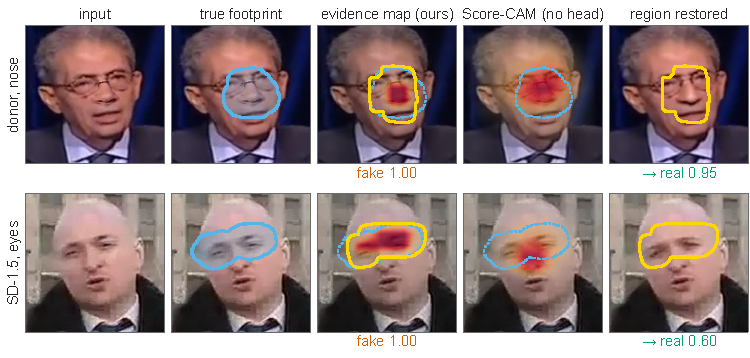
\includegraphics[width=5.0in]{fig_evidence}
\caption{Held-out part-level forgeries: input, exact footprint (blue; dashed on the maps), evidence map with the three-way
decision, Score-CAM on the same backbone without the head, and the result of restoring the region cut from the evidence map
(yellow, same area as the footprint) to the original, with the decision on it.}
\label{fig:evidence}
\end{figure}

\section{Sources that were examined and excluded}
\label{sec:excluded}
\textbf{AR beauty filters as training data.} A model trained with paired AR-filter images called 94.8\% of the filtered images
\emph{filter} with the face hull greyed out: the capture pipeline, not the face, carries the label, so AR pairs are not used for
training. As a test source they are scored in Sec.~\ref{sec:ar}, with a re-compression control and the stated upper-bound reading.
\textbf{WildDeepfake.} The 800 test frames available to us come from six sequences, which gives intervals of 0.3--0.5 AUC; not
reported. \textbf{DFDC, DFDCP.} Not available to us in a form with genuine and forged frames from the same pipeline.

\bibliographystyle{IEEEtran}
\bibliography{refs_v8}
\end{document}
